\documentclass[hidelinks, letterpaper, 12pt, oneside]{tesis}

% Paquetes para idioma
\usepackage[spanish]{babel}
\usepackage[utf8]{inputenc}
\usepackage[fixlanguage]{babelbib}

% Otros paquetes instalados
% Básicos
\usepackage[numbers,sort&compress]{natbib}
\usepackage{enumerate}
\usepackage{enumitem}
\usepackage{textcomp}
\usepackage{csquotes}
\usepackage{longtable}

%Tablas
\usepackage{caption}
\usepackage{booktabs}
\usepackage{setspace}
\usepackage{multirow}
% Para dibujar figuras
\usepackage{tikz}

% Para cambiar el color de las letras
\usepackage{color}

% Para incluir código (básico)
\usepackage{verbatim}
\usepackage{fancyvrb}
\usepackage{listings}
\definecolor{custom}{RGB}{245,245,245}
\lstset{
	language=bash,
	basicstyle=\ttfamily,
	frame=none,
	backgroundcolor=\color{custom}
}


% Para incluir hipervínculos
\usepackage{hyperref}
\usepackage{url}
\hypersetup{urlcolor=blue, colorlinks=false}

% Para más símbolos matemáticos
\usepackage{amsmath}
\usepackage{amsthm}
\usepackage{amssymb}
\renewcommand{\vec}[1]{\mathbf{#1}}
\newtheorem*{obs}{Observación}

% Para colocar teoremas en cajas
%\usepackage{mdframed}

% Para manejas la ubicacion de las figuras
\usepackage{float}
\usepackage{wrapfig}
\usepackage{graphicx}
\usepackage{subfigure}
\usepackage{varwidth,xcolor}


\usepackage{calc}
\usepackage{enumerate}
% Algoritmos y pseudoCodigos
\usepackage{amsmath}
\selectlanguage{spanish} 
\usepackage[ruled,vlined,linesnumbered,noresetcount,spanish,onelanguage]{algorithm2e} %for psuedo code

% Paquetes locales
% Puedes agregar paquetes locales (archivos .sty) en un subdirectorio % 'paquetes'.
% Utiliza la sintaxis \usepackage{paquetes/nombrePaquete}

% Todas las imágenes se cargan del subdirectorio 'img' por defecto.
\graphicspath{{imagenes/}}

% Sangrías de 3 espacios (3 veces el espacio de la x)
\parindent 3ex 

% Interlineado
\setlength{\baselineskip}{1.5pt}

% Interpárrafo
\setlength{\parskip}{16.5pt}

\topmargin 2cm

\renewcommand{\tablename}{Tabla}
\newcommand\listsymbolname{Acrónimos y Símbolos}

\begin{titlepage}
	\title{\vspace{-2cm} 
\includegraphics[width=1.2in]{./usb.png} \\[.2cm]
		\large {UNIVERSIDAD SIMÓN BOLÍVAR} \\
		\textbf{DECANATO DE ESTUDIOS PROFESIONALES \\
			COORDINACIÓN DE INGENIERIA ELECTRÓNICA}
		\vfill \large {\textbf{ODOMETRÍA VISUAL INERCIAL}}  \vfill}
	\author{Por: \\
		Luis Gabriel Lujano Chinchilla \\[1.2cm]
		\textbf{PROYECTO DE GRADO} \\
		Presentado ante la Ilustre Universidad Simón Bolívar \\
		como requisito parcial para optar al título de \\
		Ingeniero Electrónico}
	\date{Sartenejas, Marzo de 2018}
\end{titlepage}
\clearpage
\newpage
\begin{titlepage}
	\title{\vspace{-2cm} 
\includegraphics[width=1.2in]{./usb.png} \\[.2cm]
		\large UNIVERSIDAD SIMÓN BOLÍVAR \\
		\textbf{DECANATO DE ESTUDIOS PROFESIONALES \\
			COORDINACIÓN DE INGENIERIA ELECTRÓNICA}
		\vfill \large {\textbf{ODOMETRÍA VISUAL INERCIAL}}  \vfill}
	\author{Por: \\
		Luis Gabriel Lujano Chinchilla \\[1.2cm]
		Realizado con la asesoría de: \\
		José de la Cruz Cappelletto Fuentes \\
		\textbf{PROYECTO DE GRADO} \\
		Presentado ante la Ilustre Universidad Simón Bolívar \\
		como requisito parcial para optar al título de \\
		Ingeniero Electrónico}
	\date{Sartenejas, Mayo de 2018}
	
\end{titlepage}


\begin{document}
	\frontmatter
	\maketitle
	\setstretch{1.3}
	
	% Se incluye el acta de evaluación, verificar que se corresponda
	% con el formato aceptado actualmente por el Decanato.
	% Pagina del acta final
\begin{titlepage}
\begin{center}

% Upper part

\includegraphics[scale=0.5]{usb.png} \\

\textsc {\large UNIVERSIDAD SIMÓN BOLÍVAR} \\
\textsc{DECANATO DE ESTUDIOS PROFESIONALES\\
COORDINACIÓN DE INGENIERÍA ELECTRÓNICA}

\bigskip
\bigskip
\bigskip
\bigskip

% Title
\textsc{ACTA FINAL PROYECTO DE GRADO}

\bigskip
\bigskip

\textsc{\bfseries SISTEMA DE GENERACIÓN DE MOSAICOS 2D PARA ROBOTS MÓVILES A PARTIR DE VIDEO MONOCULAR}

\bigskip
\bigskip
\bigskip

\begin{minipage}{\textwidth}
\centering
Presentado por: \\
\textsc{\bfseries Victor Yovanni Garcia Carmona} \\

\bigskip
\bigskip

Este Proyecto de Grado ha sido aprobado por el siguiente jurado examinador: \\

\bigskip
\bigskip

% Despues de cada line coloca el (los) nombre(s) de
% cada uno de los integrantes del jurado.
\line(1,0){200} \\
José de la Cruz Cappelletto Fuentes\\

\bigskip
\bigskip

\line(1,0){200} \\
Novel Antonio Certad Hernandez\\


\bigskip
\bigskip

\line(1,0){200} \\
%Gerardo Fernandez López\\

\bigskip
\bigskip

% \line(1,0){200} \\
% @jurado3\\
\end{minipage}

\bigskip
\bigskip
\vfill

% Date/Fecha
{\large \bfseries Sartenejas, 7 de Mayo de 2018}

\end{center}
\end{titlepage}
 
	\begin{titlepage}
    \begin{center}

        
\includegraphics[scale=0.5]{usb.png} \\
        \textsc {\large UNIVERSIDAD SIMÓN BOLÍVAR} \\
        \textsc{DECANATO DE ESTUDIOS PROFESIONALES\\
        COORDINACIÓN DE INGENIERÍA ELECTRÓNICA}\\
        \textbf{IMPLEMENTACIÓN DE SISTEMA DE LOCALIZACIÓN Y MAPEO SIMULTÁNEO (SLAM) A PARTIR DE VISIÓN MONOCULAR Y SENSORES INERCIALES} \\
        PROYECTO DE GRADO \\
        PRESENTADO POR: \\
        Luis Gabriel Lujano Chinchilla, Carnet: 13-10775

    \end{center}
% El resumen debe ser de una sola página
\addtotoc{Resumen}
\abstract
{
	En las tareas de exploración con vehículos autonómos y teleoperados se ha generado la necesidad de desarrollar sistemas capaces de estimar el movimiento del vehículo, la trayectoria recorrida y un mapa de su entorno. Por tanto, se han desarrollado sistemas de odometría y  también de localización y mapeo simultáneo (SLAM, del inglés: \textit{Simultaneous Localization and Mapping}), que cumplan con estos objetivos, basados en diferentes tipos de sensores. En este sentido, el Grupo de Investigación y Desarrollo en Mecatrónica (GIDM) de la Universidad Simón Bolívar ha venido desarrollando un conjunto de proyectos relacionados con los sistemas de navegación de robots autónomos y de operación remota de estos,  en especial de vehículos submarinos. El siguiente trabajo presenta la implementación de un sistema de odometría visual inercial basado en una cámara monocular y una unidad de medición inercial que puede ser utilizado para estimar el movimiento de robots móviles en diferentes ambientes, y que además puede permitir la reconstrucción parcial del entorno del robot. La implementación fue realizada utilizando el Sistema Operativo Robótico (ROS, del inglés: \textit{Robot Operating System}).  Además, se presenta la implementación de un nuevo sistema que permite la generación de secuencias de datos visuales y visuales-inerciales mediante el desarrollo de un robot prototipo terrestre de bajo presupuesto.
	
    \addtocontents{toc}{\vspace{1em}}
   
    
}

% Las palabras clave son generalmente los nombres de áreas de investigación a
% los cuales está asociado el trabajo. Generalmente son tres o cuatro.
\noindent \begin{small} \textbf{Palabras clave}: odometría visual-inercial, SLAM visual-inercial, IMU, cámara monocular, robots, mapa. 
\end{small}
	
% Iniciar nueva página luego del resumen
\clearpage
\setstretch{1.3}

\end{titlepage}
 
	
	% Agradecimientos
	\acknowledgements{
		\addtocontents{toc}{\vspace{1em}}
		
		En primer lugar me gustaria agrader a Dios, por brindarme la salud y sabiduría para superar los obstaculos que he afrontado en mi carrera. También a la Universidad Simón Bolivar, que ha sido sin duda la mejor casa de estudios que pude haber tenido.
		
		Un agradecimiento muy especial a mis padres Evelyn y Yovanni por el apoyo incondicional, no solo en mi carrera sino desde que tengo uso de razón, y quienes me convirtieron en la persona que soy hoy en dia. Mas apoyo es imposible recibir.
		
		A mi tutor y quien considero como amigo José Cappelletto, de quien recibí mas que una guia a lo largo del desarrollo de este trabajo. Gracias por confiar en mi, por el apoyo, los consejps y la dedicación a lo largo de este provechoso camino. 
		
		Al profesor y tambien amigo Gerardo Fernandez por incursionarme en esta área de mi carrera, y quien me ha brindado conocimientos y experiencias muy valiosas.
		
		Gracias al laboratorio de Mecatrónica, donde recibí mucho apoyo, aliento y valiosos consejos de todos sus miembros. Gracias por hacerme sentir como uno mas de este gran grupo de investigación.
		
		Le doy las gracias a \textit{CITE}, la agrupación en la que compartí muchos buenos momentos, sin duda el lugar donde tuve la oportunidad de crecer profesionalmente y conocer a personas increíbles.
		
		Le agradezco a Andrés, Diego, Tomás, Gabriel Lesti, Nievsabel, Julio, Walter, Maria Gabriela, Carlos, Charlie, Andrea, Fabio, Ricardo y Gabiel Noya; un grupo especial de amigos que hicieron de mi experiencia universitaria la mejor de todas. Mas que unos compañeros, personas con los cuales tuve la dicha de compartir materias y los mejores momentos. Gracias por el aliento y apoyo en este duro camino muchachos, son los mejores.
		
		
	}
	\clearpage
	
	\pagestyle{fancy}
	
	% Tabla de contenidos o índice
	\lhead{\emph{Índice General}}
	\tableofcontents
	
	% Estos índices solamente se usan si el libro contiene figuras, tablas y
	% algoritmos. Si alguno de estos no se utiliza, comentar o eliminar las líneas
	% pertinentes.
	\lhead{\emph{Índice de Figuras}}
	\listoffigures
	
	\lhead{\emph{Índice de Tablas}}
	\renewcommand*\listtablename{Índice de Tablas}
	\listoftables
	
	%\lhead{\emph{Índice de Algoritmos}}
	%\renewcommand*\listalgorithmname{Índice de algoritmos}
	%\listofalgorithms
	
	\setstretch{1.5}
	\clearpage
	\lhead{\emph{Acrónimos y símbolos}}
	
	\listofsymbols{}
	{
		%\begin{longtable}{lp{0.8\textwidth}}
		
		\textbf{2D} & Dos Dimensiones\\
		
		\textbf{GIDM} & Grupo de Investigación y Desarrollo en Mecatrónica\\
		
		\textbf{ROV} & Vehículo Operado Remotamente (del inglés: Remotely Operated Vehicle)\\
		
		\textbf{AUV} & Vehículo Submarino Autónomo (del inglés: Automated Underwater Vehicle)\\
		
		\textbf{UAV} & Vehículo aéreo no tripulado (del inglés: Unmanned Aereal Vehicle)\\
		
		\textbf{SLAM} & Localización y Mapeo Simultaneo (del inglés: Simultaneous Localization and Mapping)\\
		
		\textbf{GPS} & Sistema de Posicionamiento Global (del inglés: Global Positioning System)\\
		
		\textbf{IMU} & Unidad de Medición Inercial (del inglés: Inertial Measurement Unit)\\
		
		\textbf{OpenCV} & Librería Abierta de Visión por Computadora (del inglés: Open Source Computer Vision)\\
		
		\textbf{CUDA} &  Arquitectura de Computo de Dispositivos unificados (del inglés: Compute Unified Device Architecture)\\	
		
		\textbf{SIFT} & Transformación de características invariante a la escala (del inglés: Scale Invariant Feature Transform)\\
		
		\textbf{SURF} & Transformación de caracteristicas Robusto y acelerado (del inglés: Speed-Uup Robust Features)\\
		
		\textbf{FAST} & Características de pruebas de segmentos aceleradas (del inglés: Features from Accelerated Segment Test)\\
		
		\textbf{BRIEF} & Características elementales independientes robustas binarias (del inglés: Binary Bobust Independent Elementary) Features) \\
		
		\textbf{ORB} & FAST orientado y BRIEF rotado (del inglés: Oriented for FAST and Rotated BRIEF)\\
		
		\textbf{DoG} & Diferencia de Gausianas (del inglés: Difference of Gaussians)\\
		
		\textbf{LoG} & Laplaciano de Gausianas (del inglés: Laplacian of Gaussians)\\
		
		\textbf{DoF} & Grados de Libertad (del inglés: Degrees of Freedom)\\
		
		\textbf{FLANN} & Librería de Aproximación por Vecinos mas Cercanos (del inglés: Fast Library for Aproximate Nearest Neighbors)\\
		
		\textbf{RANSAC} & Consenso de muestras aleatorias (del inglés: Random Sample Consensus)\\
		
		\textbf{RGB} & Rojo, Verde y Azul (del inglés: Red, Green and Blue)\\
		
		&\\
		\hline
		&\\	
		
		% Aquí van los símbolos
		${\rm I\!P}$ & Espacio proyectivo\\
		${\rm I\!R}$ & Espacio real\\
		
		%$\Rightarrow$ & implicación lógica\\
		%$[u:=v]$ & sustitución textual de $u$ por $v$
		%\end{longtable}
	}
	
	
	%% ----------------------------------------------------------------
	% End of the pre-able, contents and lists of things
	% Begin the Dedication page
	
	\setstretch{1.3}  % Return the line spacing back to 1.3
	
	\pagestyle{empty}  % Page style needs to be empty for this page
	
	\dedicatory{
		\textbf{Dedicatoria} \bigskip
		
		\begin{flushright}
			Para Yovanni y Evelyn.\\
			Sin ustedes no hubese podido.
		\end{flushright}
	}
	
	\addtocontents{toc}{\vspace{2em}}
	
	\mainmatter
	\pagestyle{fancy}
	
	% Se incluye el cuerpo de la tesis en este documento.
	
	% \input{./partes/introduccion}
	
	% El número de capítulos varía. En mi libro fueron cuatro (sin contar
	% introducción y conclusión).
	\chapter{Introducción}
\label{capitulo1}
\lhead{Capítulo 1. \emph{Introducción}}

En los últimos años se han logrado avances importantes en el área de navegación y exploración con robots móviles, lo que ha permitido ampliar las aplicaciones de éstos en espacios áereos, terrestres y acuáticos en diversas disciplinas, facilitando la extracción de información de estos entornos incluso en lugares de difícil acceso.

En este sentido el Grupo de Investigación y Desarrollo en Mecatrónica de la USB \textit{(GIDM)} ha venido desarrollando un conjunto de proyectos relacionados con los sistemas de navegación de robots autónomos y de operación remota de éstos desde el año 2013, donde el área de odometría y SLAM (del inglés: \textit{Simultaneous Localization and Mapping}) se ha venido trabajando con profundo interés por ser fundamental en la recopilación de información de diferentes ambientes y por abrir la puerta a la automatización de la exploración y navegación de vehículos autónomos.

\section{Antecedentes}

En el \textit{GIDM} se han realizado grandes avances en el empleo de vehículos operados remotamente \textit{ROV} (del inglés: \textit{Remotely Operated Vehicles}) y de vehículos autónomos submarinos \textit{AUV} (del inglés: \textit{Automated Underwater Vehicles}) para actividades de investigación, exploración e inspección de ambientes no estructurados.

En este sentido, en el año 2013 \textit{Certad, N.} \cite{novel} propuso como proyecto de maestría un algoritmo de localización y mapeo simultáneo para un vehículo terrestre de locomoción diferencial instrumentado con sensores exteroceptivos, realimentado por odometría, el cual utilizó Webots como herramienta de simulación y fue implementado utlizando Matlab \textregistered.


\begin{figure}[H]
	\centering
	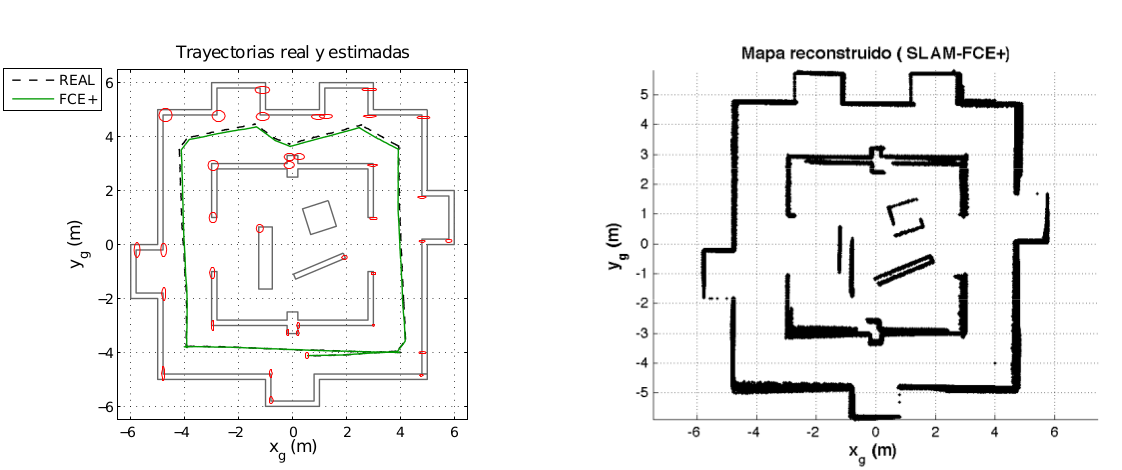
\includegraphics[width=0.7\textwidth]{Antecedentes/Certad}
	\caption{Resultados de trayectoria y reconstrucción de mapas obtenidos en \cite{novel}}
	\label{imagen:Antecedentes/Certad}
\end{figure}

En el 2017, \textit{Gonzales M.} \cite{manuel} desarrolló un sistema de reconstrucción de modelos de ambiente utilizando un sensor de Detección y Localización por Láser (LIDAR, del inglés: \textit{Laser Imaging Detection and Ranging}). Esta implementación se realizó utilizando ROS como núcleo de control y procesamiento de datos y \textit{Cartographer} como herramienta de manejo de la localización y mapeo del prototipo empleado. Los modelos reconstruidos como el presentado en la figura \ref{imagen:Antecedentes/octomaps} se realizaron utilizando estructuras probabilísticas de ocupación llamadas \textit{octomaps}, las cuales permitieron la disminución del uso de recursos de memoria en la reconstrucción de grandes entornos.


\begin{figure}[H]
	\centering
	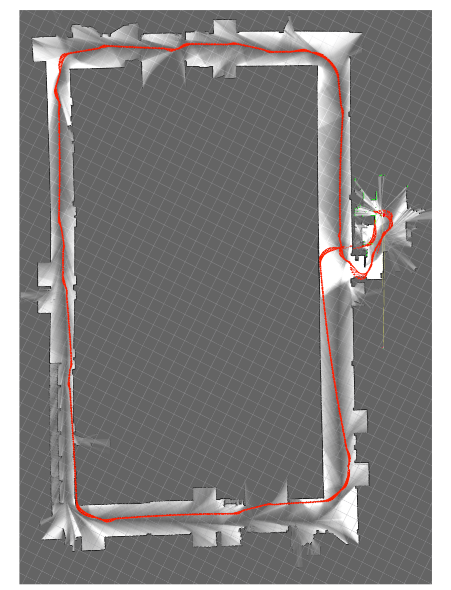
\includegraphics[width=0.3\textwidth]{Antecedentes/mapa2D}
	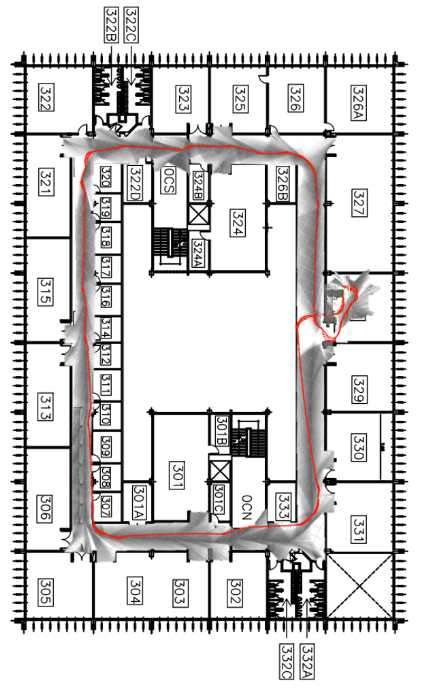
\includegraphics[width=0.3\textwidth]{Antecedentes/mapa2DReal}
	\caption[Resultados de trayectoria y reconstrucción de mapas obtenidos en \cite{manuel}] {Resultados de trayectoria y reconstrucción de mapas obtenidos en \cite{manuel}. A la izquierda se presenta el mapa original obtenido y a la derecha se presenta superpuesto al diagrama del edificio real.}
	\label{imagen:Antecedentes/mapa2D}
\end{figure}


\begin{figure}[H]
	\centering
	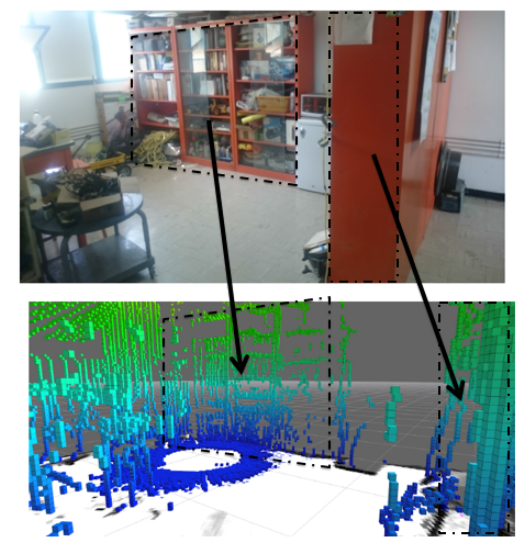
\includegraphics[width=0.7\textwidth]{Antecedentes/Octomaps}
	\caption[Reconstrucción en tres dimensiones utilizando octomaps obtenidos
	en  \cite{manuel}]{Reconstrucción en tres dimensiones utilizando octomaps obtenidos
		en  \cite{manuel}.}
	\label{imagen:Antecedentes/octomaps}
\end{figure}

En 2018,  \textit{Morales F.} \cite{fabio} desarrolló un sistema de odometría basado en cámara monocular utilizando un método directo basado en optimización de Gauss-Newton para estimar el movimiento de la cámara. La figura \ref{imagen:Antecedentes/fabio} presenta los resultados obtenidos utilizando la secuencia freiburg2 xyz del banco de datos RGB-D SLAM Dataset and Benchmark, creado por Jürgen
Sturm de la Universidad Tecnológica de Múnich.

\begin{figure}[H]
	\centering
	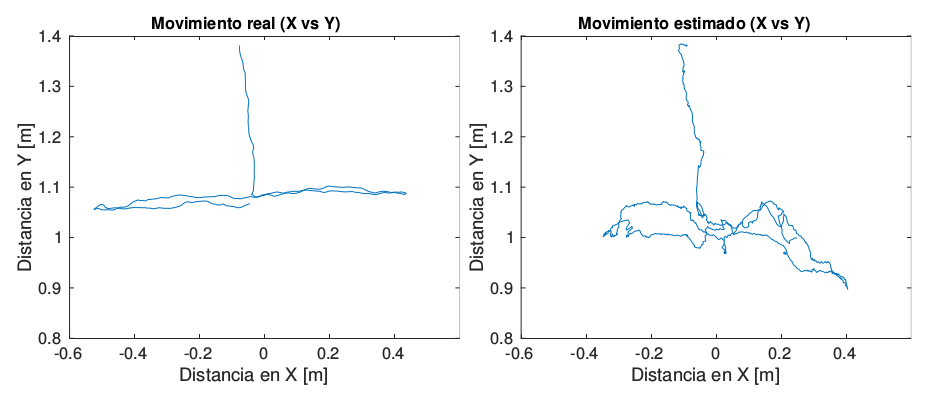
\includegraphics[width=0.7\textwidth]{Antecedentes/fabio}
	\caption[Gráficas X vs Y del movimiento de la cámara de la secuencia
	freiburg2 xyz] {Gráficas X vs Y del movimiento de la cámara de la secuencia
		freiburg2 xyz. Izquierda: gráfica del movimiento real de la cámara en X y Y.
		Derecha: gráfica del movimiento estimado de la cámara en X y Y.}
	\label{imagen:Antecedentes/fabio}
\end{figure}

 En este sentido, se tienen proyectos como el presentado por \textit{Danilo, D.} \cite{danilo}, cuyo proyecto de grado consistió en el desarrollo en un sistema de operación remota para un prototipo de robot submarino (\textit{Poseibot}), con la finalidad de implementarlo en tareas de exploración. Con objetivos similares, \textit{Said, A.} \cite{said} basó su proyecto de grado en la instrumentación y control de un robot cuadricóptero volador(\textit{UAV}) diseñado y fabricado también como parte de dicho proyecto. Este prototipo se presenta en la figura \ref{imagen:said}.
\begin{figure}[H]
	\centering
	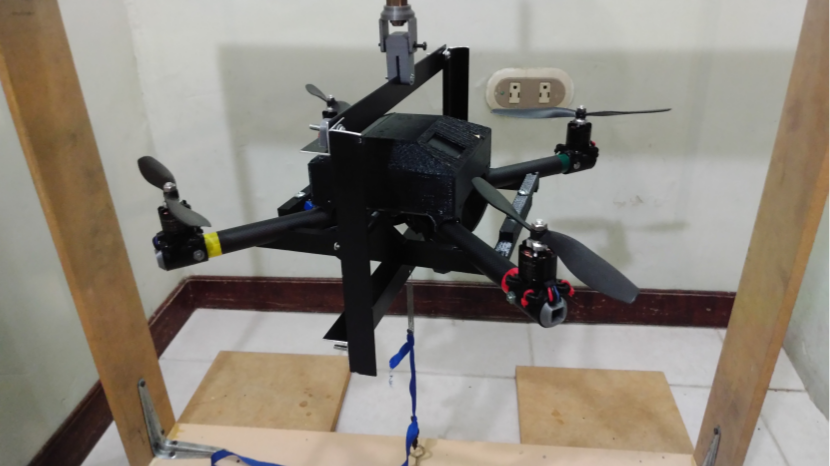
\includegraphics[width=0.7\textwidth]{Antecedentes/said}
	\caption[Prototipo UAV desarrollado en  \cite{said}]{Prototipo UAV desarrollado en  \cite{said}}
	\label{imagen:said}
\end{figure}

Adicional a estos prototipos,  el \textit{GIDM} cuentan con otras plataformas móviles como \textit{Roomba}, \textit{AmigoBot}, y un vehículo submarino OpenROV\footnote{ \url{https://www.openrov.com/products/openrov28/}}, el cual es un robot maniobrado remotamente de baja envergadura, diseñado especialmente operaciones de exploración y está dotado, entre otras cosas, con una cámara de video HD y una unidad de medición inercial.

\begin{figure}[H]
	\centering
	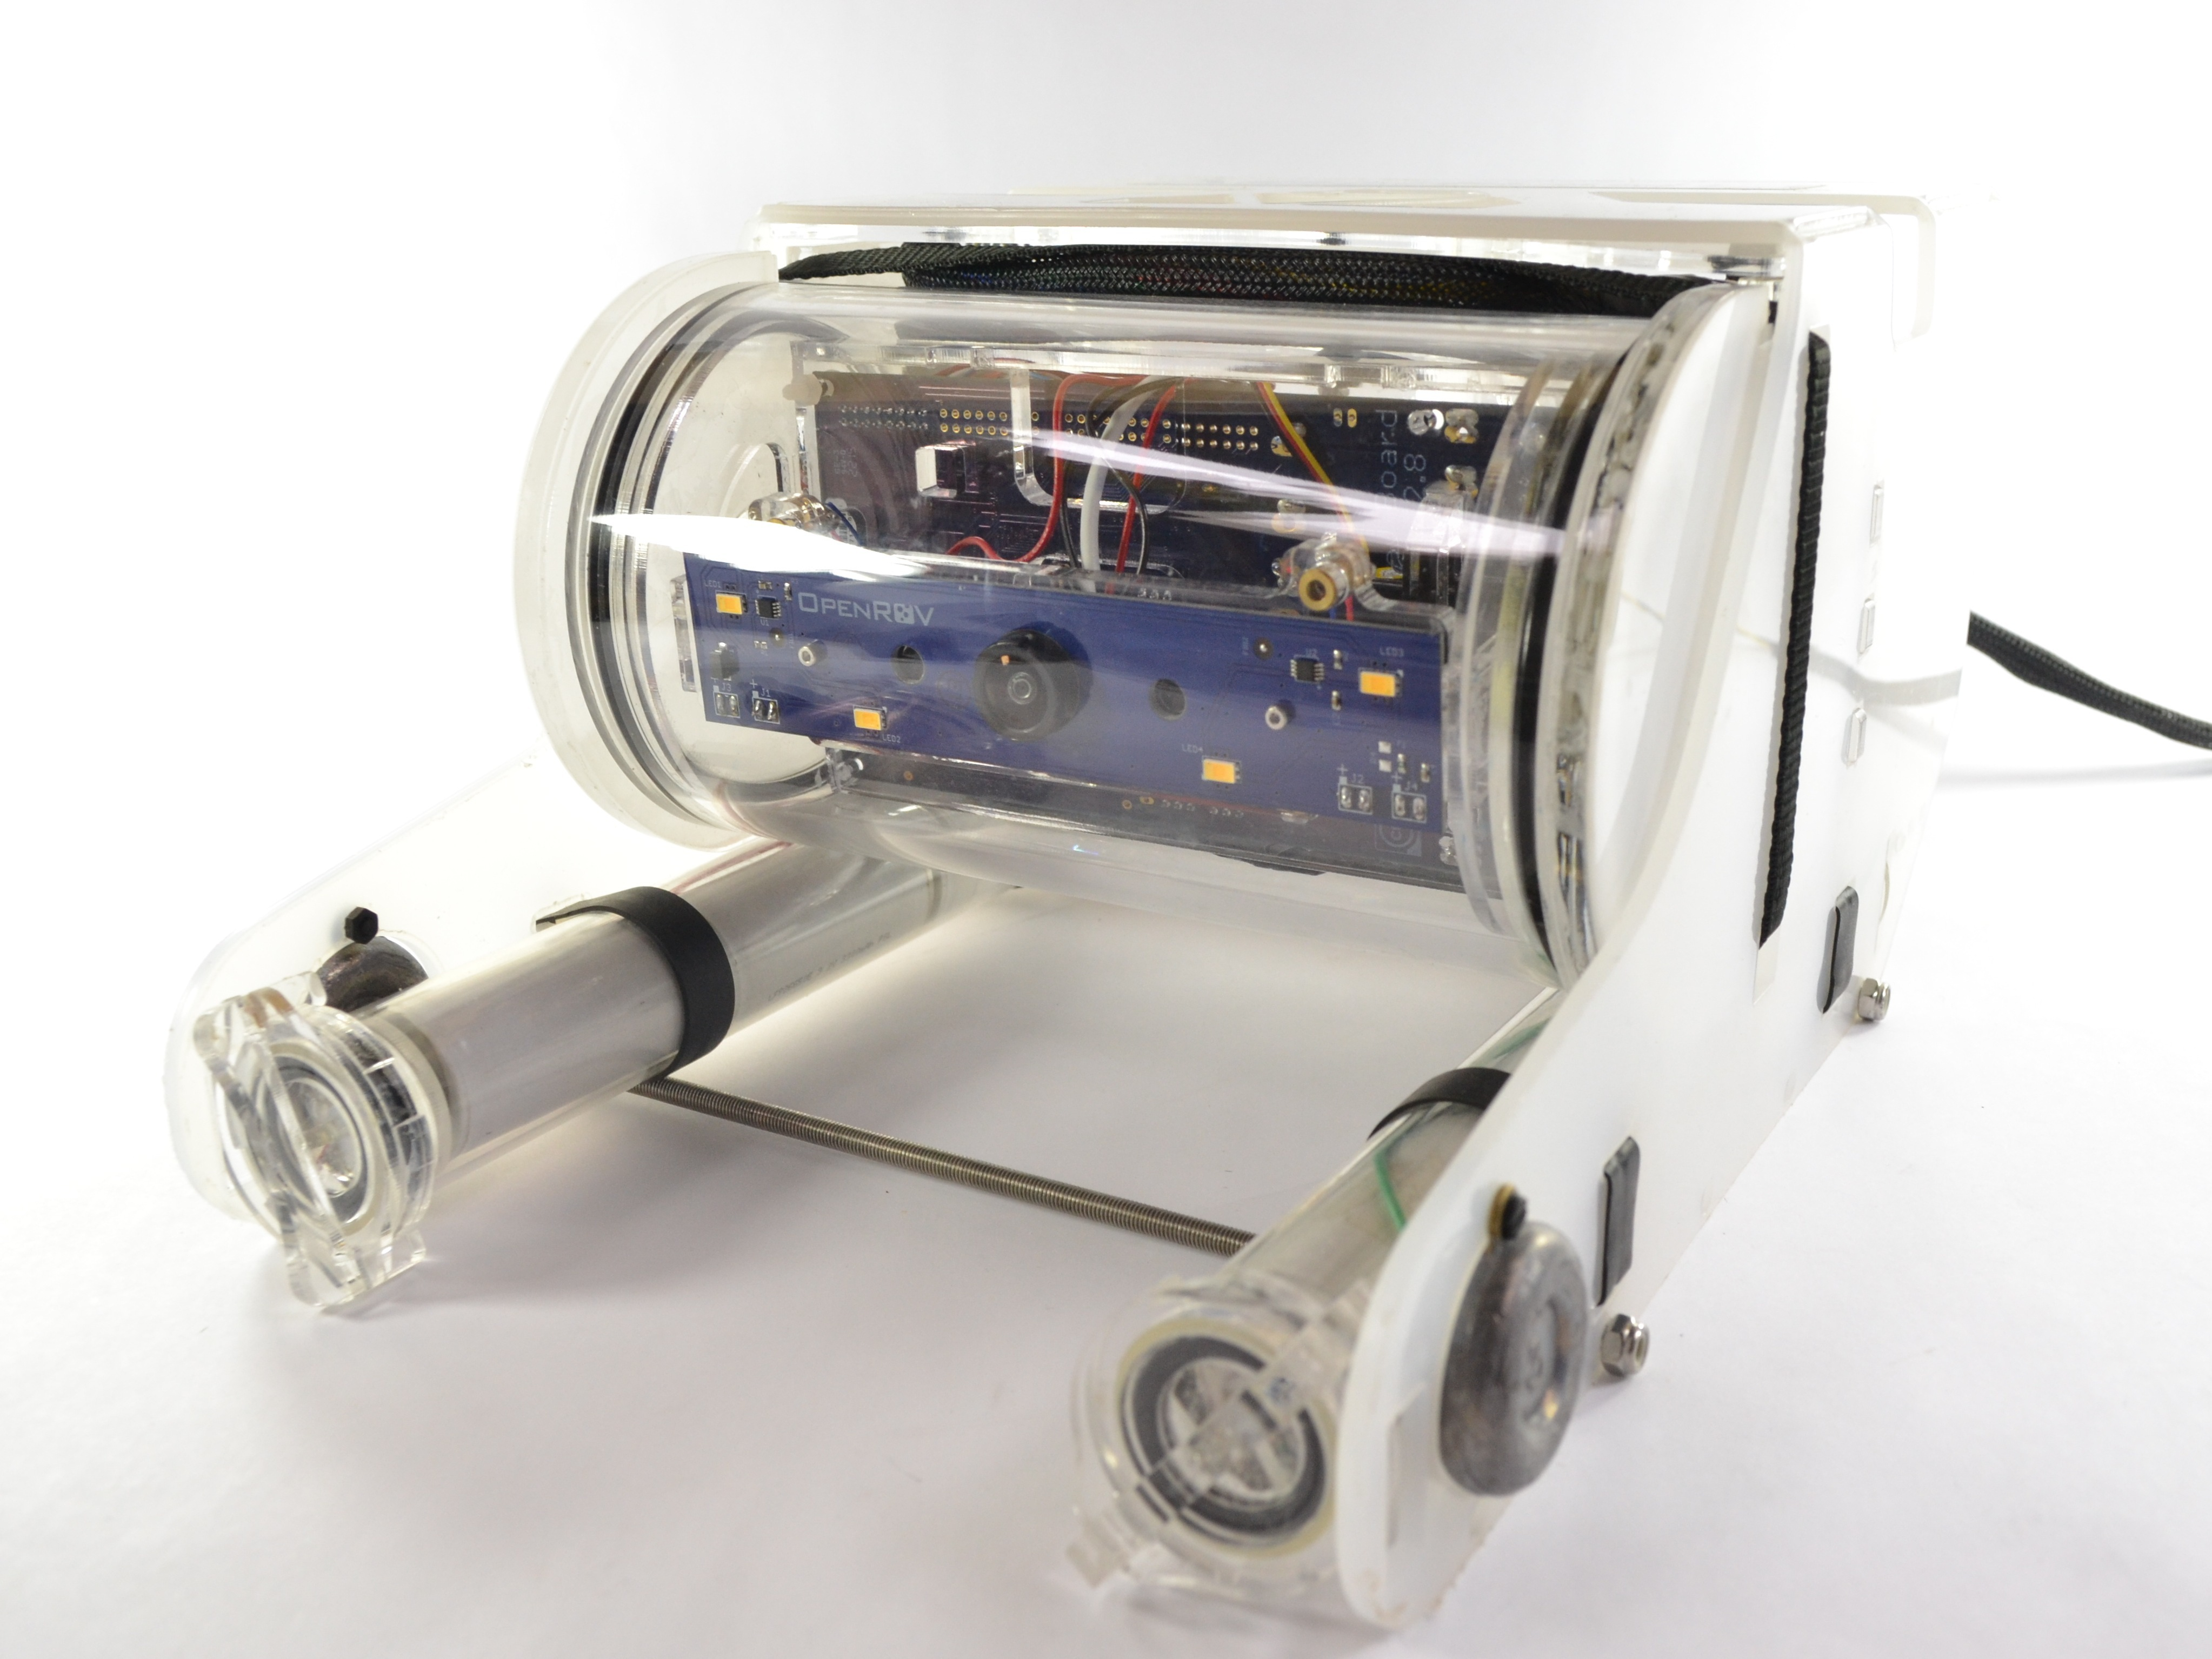
\includegraphics[width=0.7\textwidth]{openrov2}
	\caption[Robot móvil OpenROV]{Robot móvil OpenROV}
	\label{imagen:openrov}
\end{figure}

Si bien se cuenta con un conjunto de plataformas robóticas adaptadas para tareas de exploración, hasta el momento los sistemas de navegación y mapeo empleados han estado basados en GPS y telémetro láser, pero aún no se ha concluido el desarrollo de sistemas basados en visión que permitan la navegación y mapeo. La presente investigación es la primera en abordar la tarea de la reconstrucción de la superficie recorrida haciendo uso únicamente de una cámara de vídeo, sensor presente en todas las plataformas robóticas antes mencionados.

\section{Justificación y planteamiento del problema}

El Grupo de Investigación y Desarrollo en Mecatrónica de la USB ha venido desarrollando un conjunto de proyectos relacionados con los sistemas de navegación de robots autónomos y de operación remota de estos. Actualmente cuentan con un vehículo submarino OpenROV 2.8 de operación remota (ROUV, por sus siglas en inglés - Remotely Operated Underwater Vehicle) el cual posee una IMU y tiene la capacidad de transmitir videos en alta definición. Es por ello que los trabajos más recientes de este grupo han estado enfocados al área de visión por computadora con la finalidad de mejorar el desempeño y las capacidades de los sistemas de control de vehículos como el OpenROV 2.8, y para realizar exploración submarina como reconstrucción y muestreo de arrecifes, naufragios y fauna submarina. Entre estos trabajos se encuentra el proyecto de grado de Fabio Morales, en el cual se implementó un sistema de odometría visual para resolver el problema de SLAM en robots submarinos basado en una cámara monocular, y el proyecto de grado de  Armando Longart, en el cual se desarrollaron módulos de procesamiento de imágenes y video para aplicaciones subacuáticas.

Dichos trabajos permiten la posibilidad de ser integrados  y optimizados en un nuevo sistema de SLAM visual más robusto, y que además permita ser extendido para robots en diferentes entornos, automatizando la generación de las operaciones de mapeo y localización del vehículo.

\section{Objetivos}

\subsection{Objetivo General}

Analizar e implementar un sistema automatizado que permita la localización de un robot terrestre, aéreo o submarino, a través de la información capturada por una cámara monucular y una unidad de medición inercial, además de realizar un mapa de su entorno.

\subsection{Objetivos Específicos}

\begin{itemize}
	\item  Revisar la  bibliografía relacionada a la localización y mapeo simultáneo en robots móviles (aéreos, terrestres y submarinos) basados en cámara.
	\item Revisar los métodos de procesamiento de imágenes convenientes para los algoritmos de SLAM visual en función del entorno del robot móvil.
	\item Implementar un sistema de SLAM visual.
	\item Obtener la posición, trayectoria del robot móvil y  un mapa 3D aproximado de su entorno.
\end{itemize}

\section{Estructura del trabajo}

El presente trabajo se encuentra estructurado en 7 capítulos. El \textit{\textbf{Capítulo 1}} describe el problema a resolver, conjuntamente con los antecedentes más relevantes y los objetivos del proyecto.

El estado del arte de la odometría y el SLAM visual inercial es detallado en el \textit{\textbf{Capítulo 2}} donde se presentan los trabajos recientes y avances importantes en esta área de investigación. Posteriormente , en base a las técnicas y algoritmos estudiados, se propone un esquema de odometría visual inercial.


El \textit{\textbf{Capítulo 3}} inicia una revisión teórica en la que se describe el modelo de la cámara utilizado, las transformaciones de cuerpo rígido, 
el funcionamiento de los algoritmos detectores, descriptores y emparejadores de características, el filtrado de correspondencias y los filtros de fusión inercial.

La metodología implementada en este trabajo se presenta en el \textit{\textbf{Capítulo 4}}, en donde se introducen los conceptos necesarios para su implementación.

Posteriormente, en el \textit{\textbf{Capítulo 5}} se presenta el desarrollo de un dataset local visual inercial. En este capítulo se expone el diseño del robot prototipo utilizado, así como también los componentes de hardware empleados y el diagrama del esquema de recopilación de datos implementados. Además se presenta la calibración de los sensores involucrados y los resultados obtenidos para la odometría del robot.

En el \textit{\textbf{Capítulo 6}} se presenta la implementación del esquema del sistema, en donde se presentan los resultados obtenidos por dos tipos de métodos diferentes a lo largo de varias secuencias de datos. También se incluye un análisis comparativo de los resultados.


Finalmente, en el \textit{\textbf{Capítulo 7}} se presentan las conclusiones derivadas del proyecto, además de propuestas sobre recomendaciones y posibles implementaciones que pueden aportar mejoras y/o permitir la continuación del desarrollo de investigación aquí descrito.

	\chapter{Odometría y SLAM}
\label{capitulo2}
\lhead{Capítulo 2. \emph{Odometría y SLAM}}

En este capítulo se presenta una revisión teórica del estado actual de las investigaciones que se han realizado en el área de Odometría visual, SLAM visual, y sus vertientes en las que se fusionan los datos inerciales.

\section{Estado del arte}

En los últimos años se han presentado diferentes alternativas para estimar de forma efectiva el movimiento que efectúa un robot y además lograr realizar un mapa de su entorno.


\section{SLAM visual}

\section{Fusión visual-inercial }
A lo largo de los años se han utilizado diferentes tipos de sensores y sus combinaciones para realizar la localización y mapeo simultáneo (SLAM) de un robot móvil en su entorno. Entre éstos se encuentran láseres de rango, sonares, sistemas de posicionamiento global (GPS), unidades de medición inercial (IMU) y cámaras monoculares, estereoscópicas, y RGB-D.\\

Cada tipología en la que son empleados estos sensores tiene sus limitaciones. Por ejemplo, los sistemas en que los se utiliza GPS están restringidos a ser utilizados al aire libre, lo que conlleva a que no puedan ser implementados en vehículos submarinos. Los láseres ofrecen información precisa del entorno pero tienen problemas en superficies reflectivas o absorbentes, además que pueden representar un alto costo,  y  ser lo suficientemente pesados como para ser descartados en aplicaciones con  vehículos aéreos. Por su parte, las medidas de sonares que son aplicados en espacios terrestres pueden tener alta incertidumbre ya que depende de la forma de las superficies y de su orientación relativa al sensor, mientras que las unidades de medición inercial presentan deriva y ruido en sus mediciones. En el caso de las cámaras, la  calidad de sus datos tienen una alta dependencia a las condiciones de iluminación. \\

La implementación de estas últimas en sistemas de localización y mapeo simultáneo ha tenido gran atención en los últimos años debido a su capacidad para capturar una gran cantidad de información sobre el entorno. Es por esto que se han desarrollado métodos de SLAM visual basados tanto en cámaras monoculares como estereoscópicas, utilizando para ello métodos directos, a través de la detección y emparejamiento de características en las imágenes; método indirectos, basados en el calculo del error fotométrico entre imágenes; y semi-directos, utilizando una combinación de métodos directos e indirectos.\\

Sin embargo, estos sistemas presentan debilidades. Los métodos de SLAM con cámaras monoculares presentan problemas de ambiguedad ante la escala, mientras que  los estereoscópicos están limitados por la relación entre la profundidad de la escena y la distancia entre las cámaras. \\

Es por ello que con el objetivo de generar un sistema más robusto en el que se puede complementar la información disponible entre sensores y compensar sus debilidades, se han propuesto esquemas basados en la fusión visual-inercial, en la que se pueden emplear cámaras estéreos o monoculares junto a una unidad de medición inercial, ofreciendo además una buena relación entre costo, peso, espacio ocupado y consumo de energía, que permite que puedan ser empleados en robots terrestres, aéreos y submarinos.\\

El núcleo de esta fusión se encuentra basado en la complementariedad que tienen estos sensores. Por ejemplo, las cámaras son precisas en movimientos lentos, en los cuales las medidas aceleración y velocidad angular provenientes de la IMU tienen mayor incertidumbre. En el caso de movimientos rápidos, sucede justo lo contrario: la IMU presenta menor incertidumbre en sus medidas mientras que las imágenes captadas por la cámara se distorsionan por efectos como el blur. \\

Por otro lado,  las frecuencias de muestreo de las cámaras convencionales están el orden de las decenas de Hertz, mientras que las de la IMU pueden alcanzar las centenas de Hertz, con lo que se  obtiene información inercial adicional entre dos imágenes, que al ser integrada permite establecer restricciones de movimiento,  logrando de esta forma alcanzar una mejor estimación del estado del robot frente a su entorno., requiriendo un menor tiempo de cómputo. \\
\section{Odometría visual}
\section{SLAM}


\subsection{OKVIS}

El sistema de SLAM visual-inercial basado en keyframes y optimización no lineal (OKVIS)  es un enfoque desarrollado en 2013 en el laboratorio d de sistemas autónomos de la Escuela Politécnica Federal de Zúrich (ETH), en Suiza.

Este enfoque integra de forma estrecha las medidas de la IMU y los keyframes provenientes de visión estéreo, utilizando optimización de Gauss-Newton para minimizar el error . El detector que se empleó es el detector de Harriz multiescala con optimización en el espacio SSE , combinado con el descriptor BRISK. 

La visión estereo es utilizada para realizar la triangulación de los puntos característicos en cada frame, los cuales son insertados a un mapa local. Luego se aplica el algoritmo de fuerza bruta para encontrar la correspondecia con el mapa global de landmarks. En este caso, se utiliza outlier rejection aplicnado es test de chi-cuadrado a las coordenadas de la imagen utilizando las poses obtenidas previamente mediante la integración de las medidas de la IMU.
En este enfoque se utiliza una ventana deslizante para mantener los frames más reciente, y la selección de keyframes se basa en una medida heuristica: si la razón entre el area ocupado por todo los puntos emparejados contra el area ocupaa por todos los puntos detectados está entre 50 a 60, el frame es considerado como keyframe.



Debido a que se utiliza keyframes, se pueden tener frames separados arbitrariamente en tiempo. Los keyfra

En este trabajo comparan las estimaciones realizadas entre los diferentes acoples: el visual, el ligeramente acoplado y el estrechamente acoplado.


\begin{figure}[H]
	\centering
	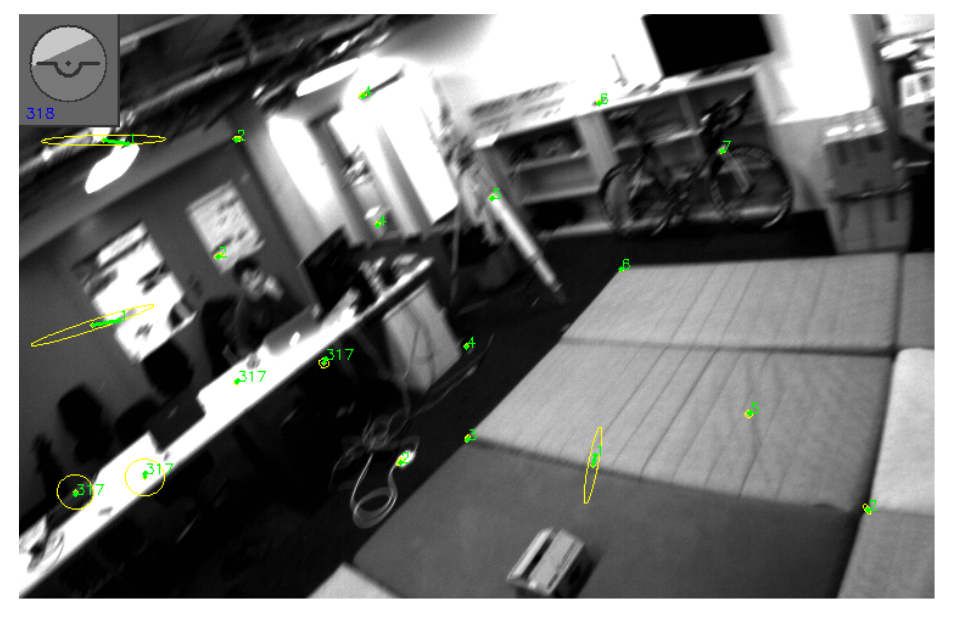
\includegraphics[scale=0.4]{EstadoDelArte/Rovio/RovioEstimacion.png}
	\caption{Captura del entorno de trabajo de la odometría visual-inercial. Las elipses encierran la zona donde se predice la localización de las características. Las elipses estrechas corresponden a las características de mayor incertidumbre, entre las que se encuentran las características nuevas. Luego de la estimación efectuada por el EKF, la localización de la característica es mostrada como un punto verde. Los números en color verde corresponden al número de veces que ha sido seguida la características (1 si es una nueva característica).}
	\label{fig:RovioEstimacion}
\end{figure}


\begin{figure}[H]
	\centering
	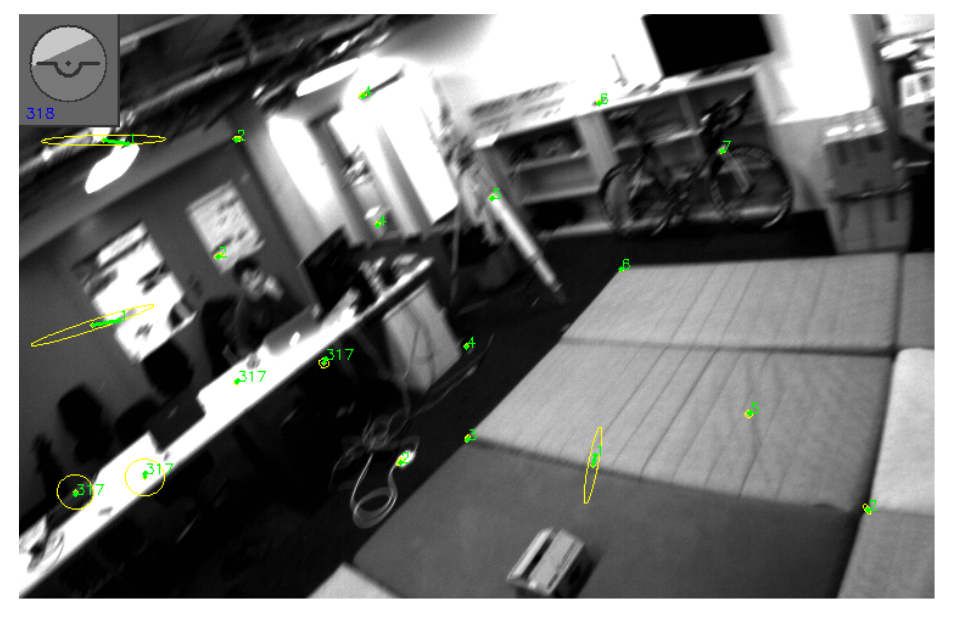
\includegraphics[scale=0.4]{EstadoDelArte/Rovio/RovioEstimacion.png}
	\caption{Captura del entorno de trabajo de la odometría visual-inercial. Las elipses encierran la zona donde se predice la localización de las características. Las elipses estrechas corresponden a las características de mayor incertidumbre, entre las que se encuentran las características nuevas. Luego de la estimación efectuada por el EKF, la localización de la característica es mostrada como un punto verde. Los números en color verde corresponden al número de veces que ha sido seguida la características (1 si es una nueva característica).}
	\label{fig:RovioEstimacion}
\end{figure}



\begin{figure}[H]
	\centering
	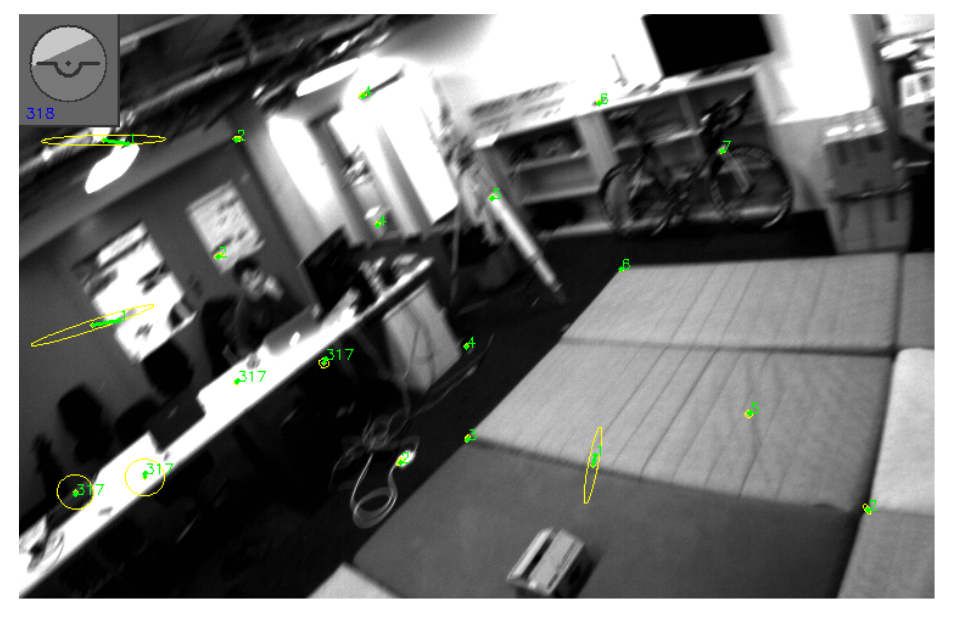
\includegraphics[scale=0.4]{EstadoDelArte/Rovio/RovioEstimacion.png}
	\caption{Captura del entorno de trabajo de la odometría visual-inercial. Las elipses encierran la zona donde se predice la localización de las características. Las elipses estrechas corresponden a las características de mayor incertidumbre, entre las que se encuentran las características nuevas. Luego de la estimación efectuada por el EKF, la localización de la característica es mostrada como un punto verde. Los números en color verde corresponden al número de veces que ha sido seguida la características (1 si es una nueva característica).}
	\label{fig:OkvisResultados}
\end{figure}

\subsection{ROVIO}

La Odometría Visual-Inercial Robusta (ROVIO, del inglés: Robust Visual Inertial Odometry) es un algoritmo desarrollado en 2015 en el laboratorio de sistemas autónomos del ETH.

Este algoritmo utilizan directamente como error la intensidad de los píxeles, utilizando parches en las  imágenes y aplicando la estructura piramidal de 4 niveles y manteniendo un alto nivel de robustez. Los parches utilizados están fuertemente acoplados con un filtro Kalman Extendido (EKF, del inglés: Extended Kalman Filters) y los landmarks 3D son siempre estimados con respecto a la pose actual de la cámara. lo que es conocido como el enfoque robocéntrico. Además, estos landmarks son parametrizados para lograr una na forma compacta de representación y de esa forma mejorar el desempeño computacional del algoritmo. 

El filtro empleado fusiona los datos de aceleración y velocidad angular de la IMU, y los parámetros extrinsecos de la cámara y los biases de la IMU son coestimados. 

Las características utilizadas aquí se refieren directamente a un píxel dentro de un parche de la imagen. El propósito del filtro es predecir la ubicación de las características en la siguiente imagen y de esta forma, extraer un parche de la siguiente imagen, y estimar la mejor transformación de cuerpo rígido que minimice el error de intesidad entre los parches. 

Cuando la predicción de la ubicación del parche se encuentra fuera de la región de la imagen, es eliminada la características y se crean nuevas. También puede ser eliminada la caracteristica en función de sus estadísticas, las cuales están asociadas al grado de certidumbre o varianza. La imagen \ref{fig:RovioEstimacion} muestra un ejemplo de esto.

\begin{figure}[H]
	\centering
	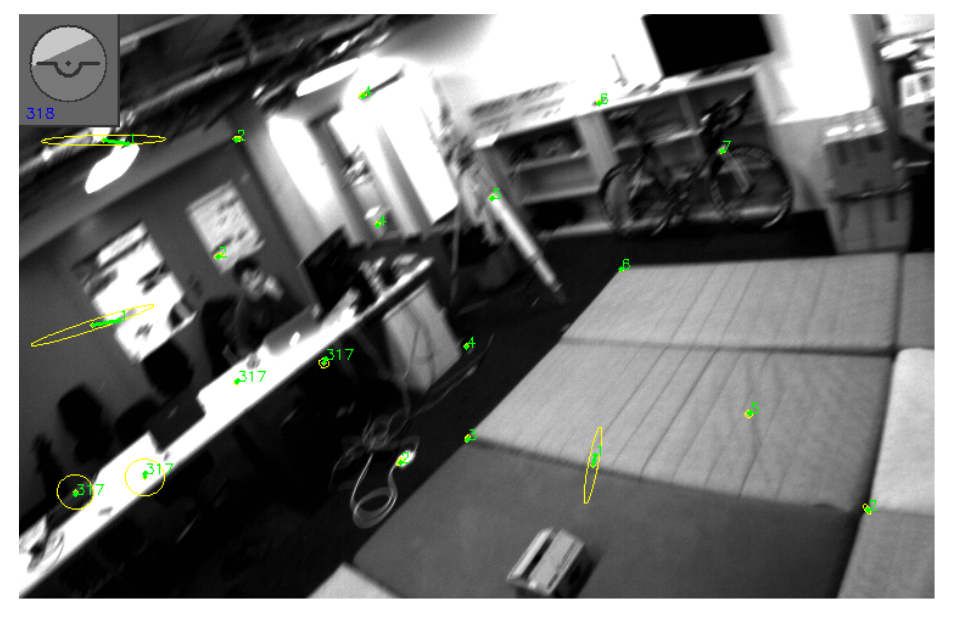
\includegraphics[scale=0.4]{EstadoDelArte/Rovio/RovioEstimacion.png}
	\caption{Captura del entorno de trabajo de la odometría visual-inercial. Las elipses encierran la zona donde se predice la localización de las características. Las elipses estrechas corresponden a las características de mayor incertidumbre, entre las que se encuentran las características nuevas. Luego de la estimación efectuada por el EKF, la localización de la característica es mostrada como un punto verde. Los números en color verde corresponden al número de veces que ha sido seguida la características (1 si es una nueva característica).}
	\label{fig:RovioEstimacion}
\end{figure}


Este enfoque no requiere una etapa de inicialización, por lo que es posible utilizar este sistema de estimación de estados directamente.


Para evaluar la robustez de este algoritmo, el laboratorio utilizo su propio vehiculo aerio, equipado con dos cámaras con disparo global sincronizadas con el trigger de la imu. En el contexto del trabajo sólo fue utilizado una de las cámaras. El Ground truth fue proveido por un sistema externo de captura de movimiento. En esta configuración se fijó la tasa de las medidas de la IMU a 200Hz y la de las cámaras a 20Hz. Los resultados de la estimación se presentan en las figuras \ref{fig:RovioOrientacion} y  \ref{fig:RovioTrayectoria}.



\begin{figure}[H]
	\centering
	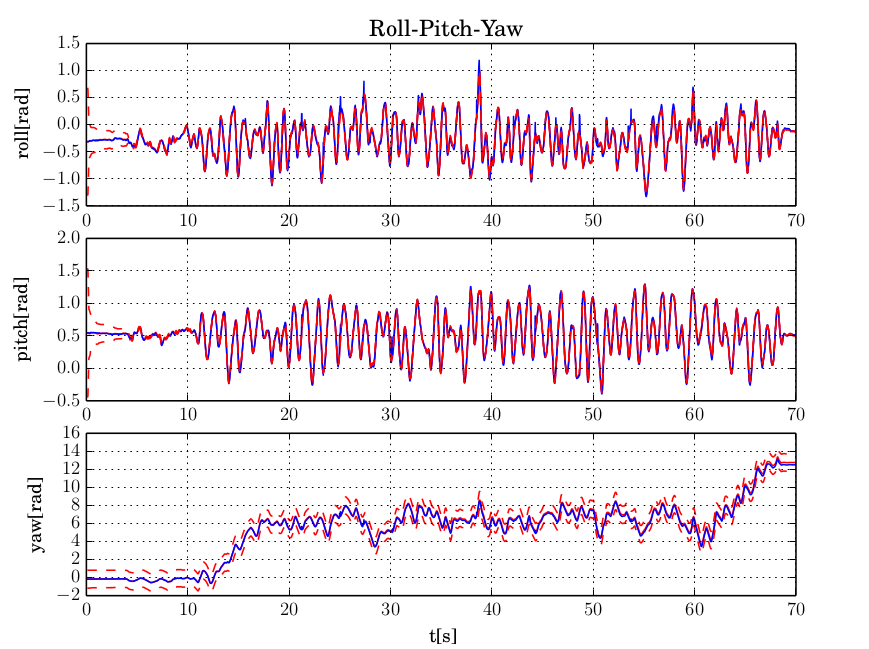
\includegraphics[scale=0.4]{EstadoDelArte/Rovio/RovioOrientacion.png}
	\caption{Ángulos RPY estimados (rojo) del UAV comparado con los obtenidos mediante el sistema de captura de movimiento (azul). La incertidumbre de la estimación se muestra con lineas discontinuas. }
	\label{fig:RovioOrientacion}
\end{figure}


\begin{figure}[H]
	\centering
	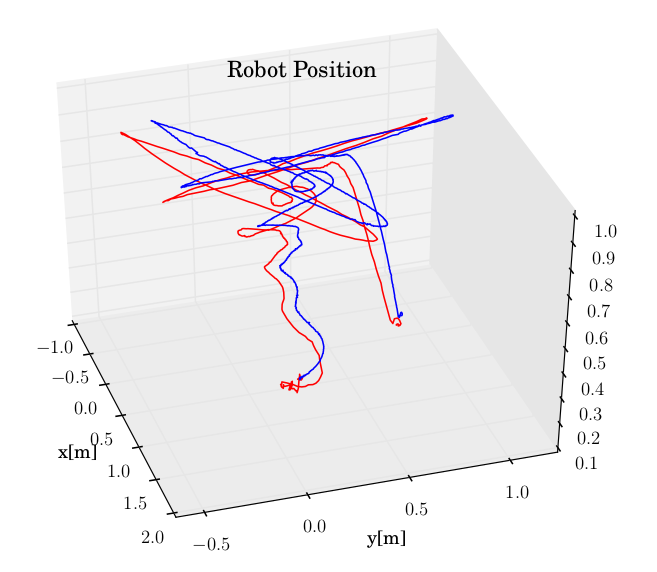
\includegraphics[scale=0.4]{EstadoDelArte/Rovio/RovioTrayectoria.png}
	\caption{Trayectoria estimada (rojo) del UAV comparado con el groundtruth (azul) proveniente del sistema de captura de movimiento .}
	\label{fig:RovioTrayectoria}
\end{figure}




\section{Fusión visual-inercial }
A lo largo de los años se han utilizado diferentes tipos de sensores y sus combinaciones para realizar la localización y mapeo simultáneo (SLAM) de un robot móvil en su entorno. Entre éstos se encuentran láseres de rango, sonares, sistemas de posicionamiento global (GPS), unidades de medición inercial (IMU) y cámaras monoculares, estereoscópicas, y RGB-D.\\

Cada tipología en la que son empleados estos sensores tiene sus limitaciones. Por ejemplo, los sistemas en que los se utiliza GPS están restringidos a ser utilizados al aire libre, lo que conlleva a que no puedan ser implementados en vehículos submarinos. Los láseres ofrecen información precisa del entorno pero tienen problemas en superficies reflectivas o absorbentes, además que pueden representar un alto costo,  y  ser lo suficientemente pesados como para ser descartados en aplicaciones con  vehículos aéreos. Por su parte, las medidas de sonares que son aplicados en espacios terrestres pueden tener alta incertidumbre ya que depende de la forma de las superficies y de su orientación relativa al sensor, mientras que las unidades de medición inercial presentan deriva y ruido en sus mediciones. En el caso de las cámaras, la  calidad de sus datos tienen una alta dependencia a las condiciones de iluminación. \\

La implementación de estas últimas en sistemas de localización y mapeo simultáneo ha tenido gran atención en los últimos años debido a su capacidad para capturar una gran cantidad de información sobre el entorno. Es por esto que se han desarrollado métodos de SLAM visual basados tanto en cámaras monoculares como estereoscópicas, utilizando para ello métodos directos, a través de la detección y emparejamiento de características en las imágenes; método indirectos, basados en el calculo del error fotométrico entre imágenes; y semi-directos, utilizando una combinación de métodos directos e indirectos.\\

Sin embargo, estos sistemas presentan debilidades. Los métodos de SLAM con cámaras monoculares presentan problemas de ambiguedad ante la escala, mientras que  los estereoscópicos están limitados por la relación entre la profundidad de la escena y la distancia entre las cámaras. \\

Es por ello que con el objetivo de generar un sistema más robusto en el que se puede complementar la información disponible entre sensores y compensar sus debilidades, se han propuesto esquemas basados en la fusión visual-inercial, en la que se pueden emplear cámaras estéreos o monoculares junto a una unidad de medición inercial, ofreciendo además una buena relación entre costo, peso, espacio ocupado y consumo de energía, que permite que puedan ser empleados en robots terrestres, aéreos y submarinos.\\

El núcleo de esta fusión se encuentra basado en la complementariedad que tienen estos sensores. Por ejemplo, las cámaras son precisas en movimientos lentos, en los cuales las medidas aceleración y velocidad angular provenientes de la IMU tienen mayor incertidumbre. En el caso de movimientos rápidos, sucede justo lo contrario: la IMU presenta menor incertidumbre en sus medidas mientras que las imágenes captadas por la cámara se distorsionan por efectos como el blur. \\

Por otro lado,  las frecuencias de muestreo de las cámaras convencionales están el orden de las decenas de Hertz, mientras que las de la IMU pueden alcanzar las centenas de Hertz, con lo que se  obtiene información inercial adicional entre dos imágenes, que al ser integrada permite establecer restricciones de movimiento,  logrando de esta forma alcanzar una mejor estimación del estado del robot frente a su entorno., requiriendo un menor tiempo de cómputo. \\
\section{EuRoC MAV Dataset}
El conjunto de datos de prueba empleado en este trabajo corresponde al al EuRoC MAV Dataset \cite{0}, el cual es un dataset de referencia que es utilizado para evaluar diferentes algoritmos de SLAM visual-inercial y que dispone de 11 secuencias de datos. \\


El EuRoC MAV Dataset contiene imágenes estéreo sincronizadas con las medidas de la IMU,  y un groundtruth preciso que es estimado utilizando el láser Leica y el sistema de captura de movimiento Vicon. Los datos fueron recolectados utilizando robot aéreo el cual se presenta en la figura \ref{fig:robotEuroc}. \\

\begin{figure}[H]
	\centering
	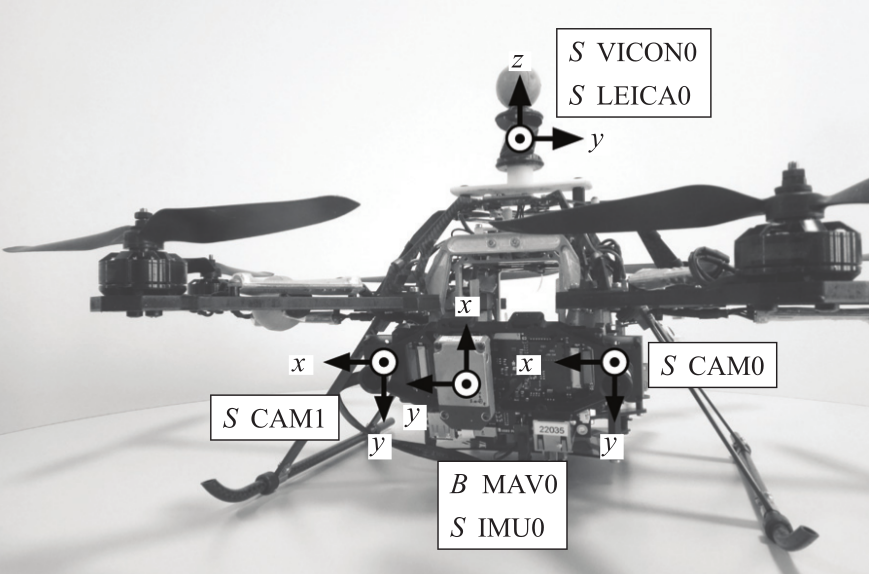
\includegraphics[scale=0.4]{Implementacion/robotEuroc.png}
	\caption{Robot aéreo empleado en la recolección de datos en el EuRoC MAV Dataset .}
	\label{fig:robotEuroc}
\end{figure}

Las cámaras empleadas en estas secuencias capturan datos a 20Hz, mientras que la IMU opera a 200Hz. En nuestro caso, se utilizará la cámara CAM0 de la figura \ref{fig:robotEuroc}. Esta cámara se encuentra sincronizada con la IMU tal como se presenta en la figura \ref{fig:sincronizacionEuroc}. En un tiempo $t_k$ se captura tanto la imagen de la cámara, como las medidas de aceleración y velocidad angular provenientes de la IMU. El tiempo $t_c$ representa el lapso de tiempo entre la captura de dos imágenes y corresponde con 50 ms. En este caso, se tienen $n = 10$ medidas de la IMU entre cada captura de la cámara. \\

\begin{figure}[H]
	\centering
	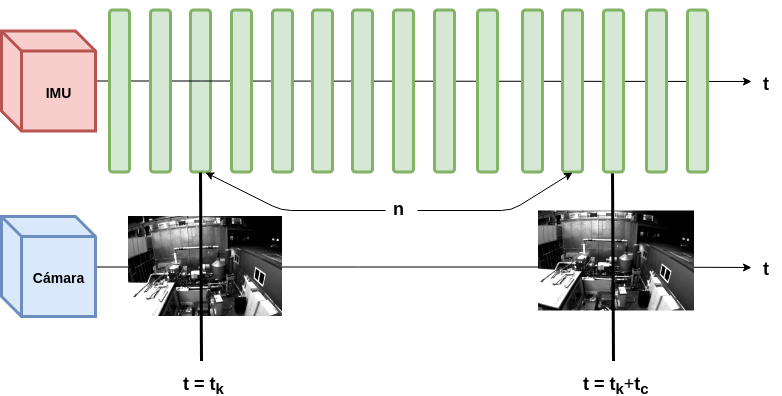
\includegraphics[scale=0.4]{Implementacion/DiagramaIMUCamara.png}
	\caption{Sincronización entre la IMU y la cámara.}
	\label{fig:sincronizacionEuroc}
\end{figure}

También se dispone de la calibración de los parámetros intrísecos y extrinsecos del sistema. En la figura \ref{fig:extrinsecosEuroc} se muestran los parámetros extrínsecos relevantes para este trabajo. En este caso, se utiliza la transformación de cuerpo rígido $T{B-CAM0}$, que relaciona el sistema de referencia de la IMU (Body, B) y el sistema de referencia de la cámara CAM0. 



\begin{figure}[H]
	\centering
	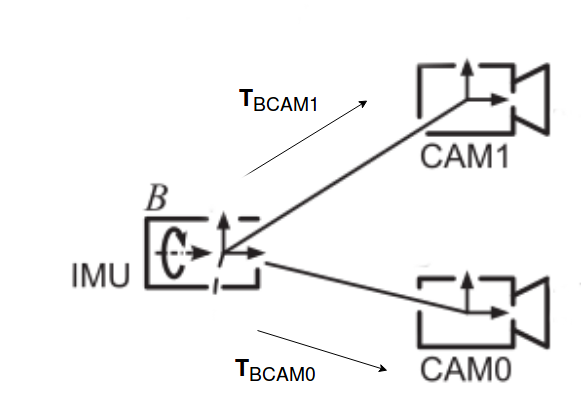
\includegraphics[scale=0.4]{Euroc/Enlaces.png}
	\caption{Parámetros extrínsecos del sistema}
	\label{fig:extrinsecosEuroc}
\end{figure}

Las secuencias de este conjuntos de datos se encuentran clasificadas en "fácil", "media", y "difícil",  en función de la media de la velocidad lineal y angular del robot utilizado y de las condiciones visuales y niveles de iluminación. En la figura \ref{fig:tablaDeCaracteristicas} se presentan las características de las secuencias. 

\begin{figure}[H]
	\centering
	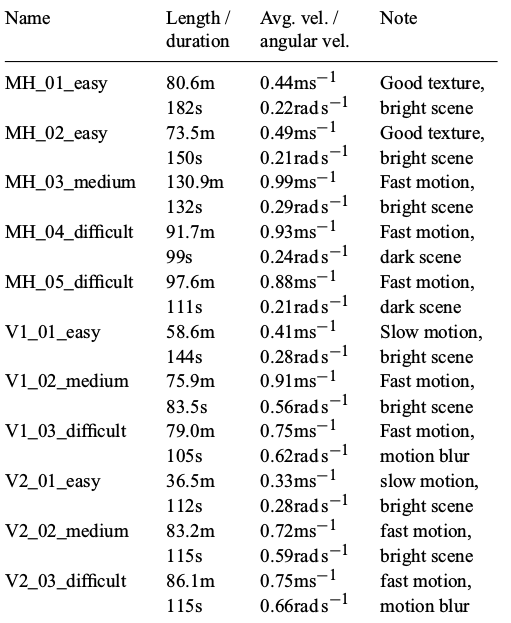
\includegraphics[scale=0.4]{Euroc/TabladeCaracteristicas.png}
	\caption{Características de las secuencias de datos del EuRoC MAV Dataset}
	\label{fig:tablaDeCaracteristicas}
\end{figure}



Este conjunto de datos fue recolectado en dos tipos de ambiente. El primer ambiente se presenta en la figura \ref{fig:machineHall} y  corresponde a una sala de máquinas en el cual fueron recolectadas 5 secuencias de datos (MH\_01\_easy, MH\_02\_easy, MH\_03\_medium, MH\_04\_difficult, MH\_05\_difficult). \\

En la figura \ref{fig:vicon} se muestra el segundo ambiente correspondiente a una habitación en el que se tomaron 6 secuencias de datos (V1\_01\_easy, V1\_02\_medium, V1\_03\_difficult, V2\_02\_easy, V2\_02\_medium, V2\_03\_difficult). En estas secuencias se dispone de la nube de puntos de la habitación, la cual fue generada a través de la fusión de las medidas tomadas con el láser Leica, y se presentan en la figura \ref{fig:pointcloudEuroc}.\\

\begin{figure}[H]
	\centering
	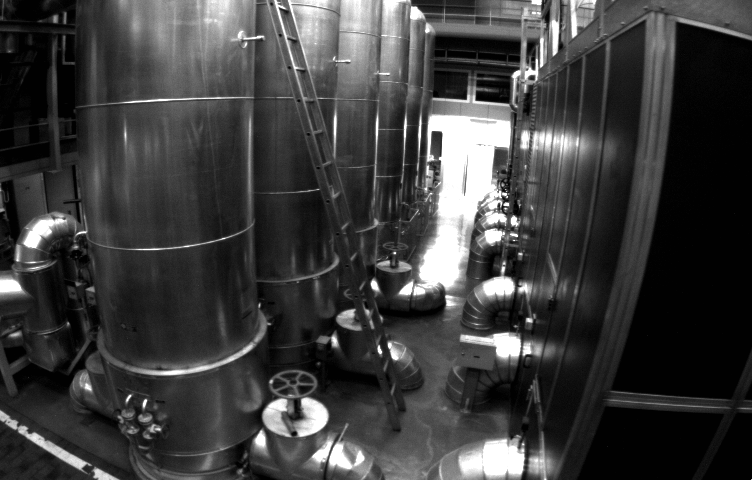
\includegraphics[scale=0.2]{Euroc/MachineHall1.png}
	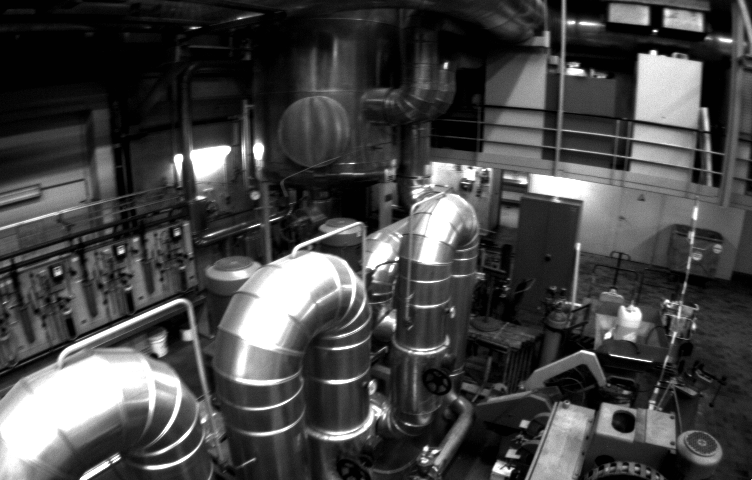
\includegraphics[scale=0.2]{Euroc/MachineHall2.png}
	\caption{Imágenes de la secuencia de datos correspondiente a la sala de máquinas.}
	\label{fig:machineHall}
\end{figure}


\begin{figure}[H]
	\centering
	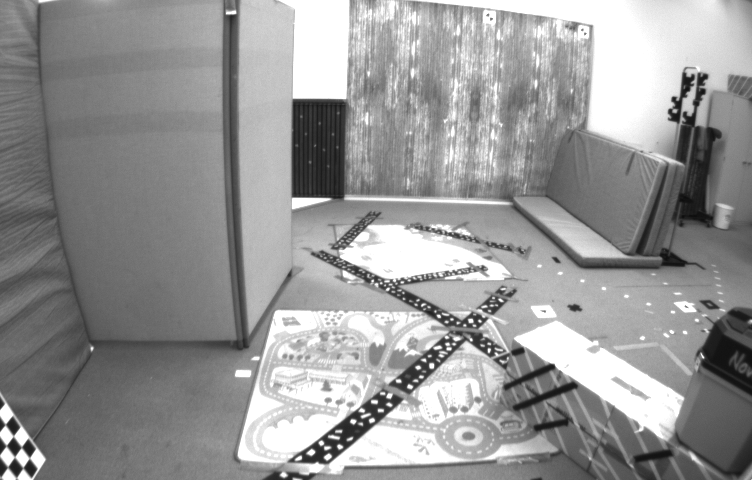
\includegraphics[scale=0.2]{Euroc/Vicon0.png}
	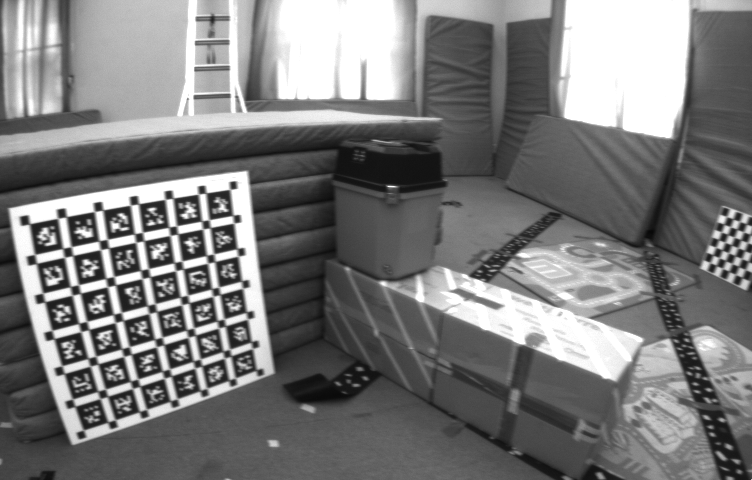
\includegraphics[scale=0.2]{Euroc/Vicon1.png}
	\caption{Imágenes de la secuencia de datos correspondiente a la habitación Vicon.}
	\label{fig:vicon}
\end{figure}


\begin{figure}[H]
	\centering
	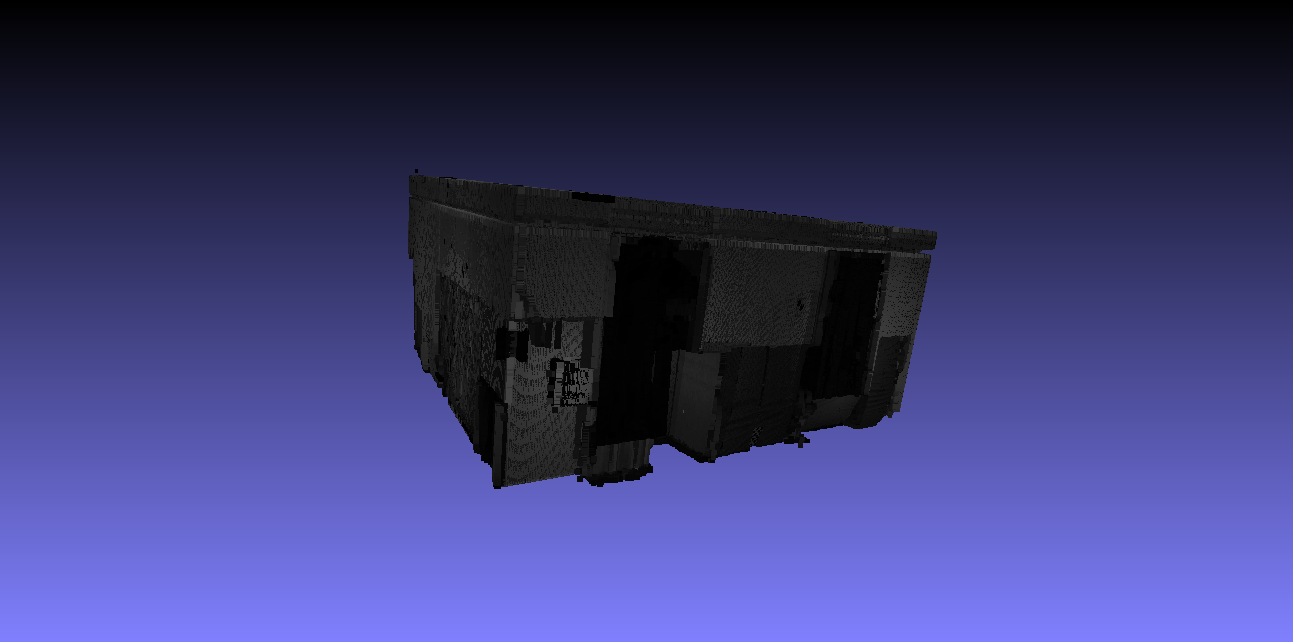
\includegraphics[scale=0.2]{Euroc/Pointcloud0.png}
	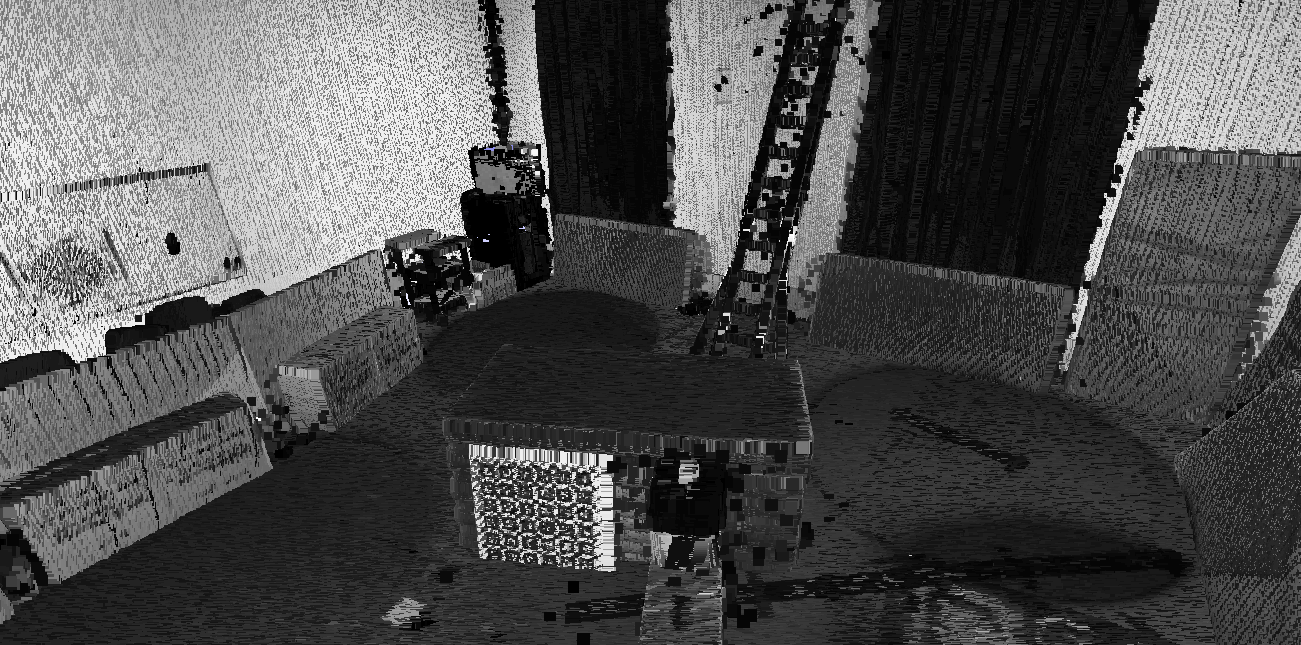
\includegraphics[scale=0.2]{Euroc/Pointcloud1.png}
	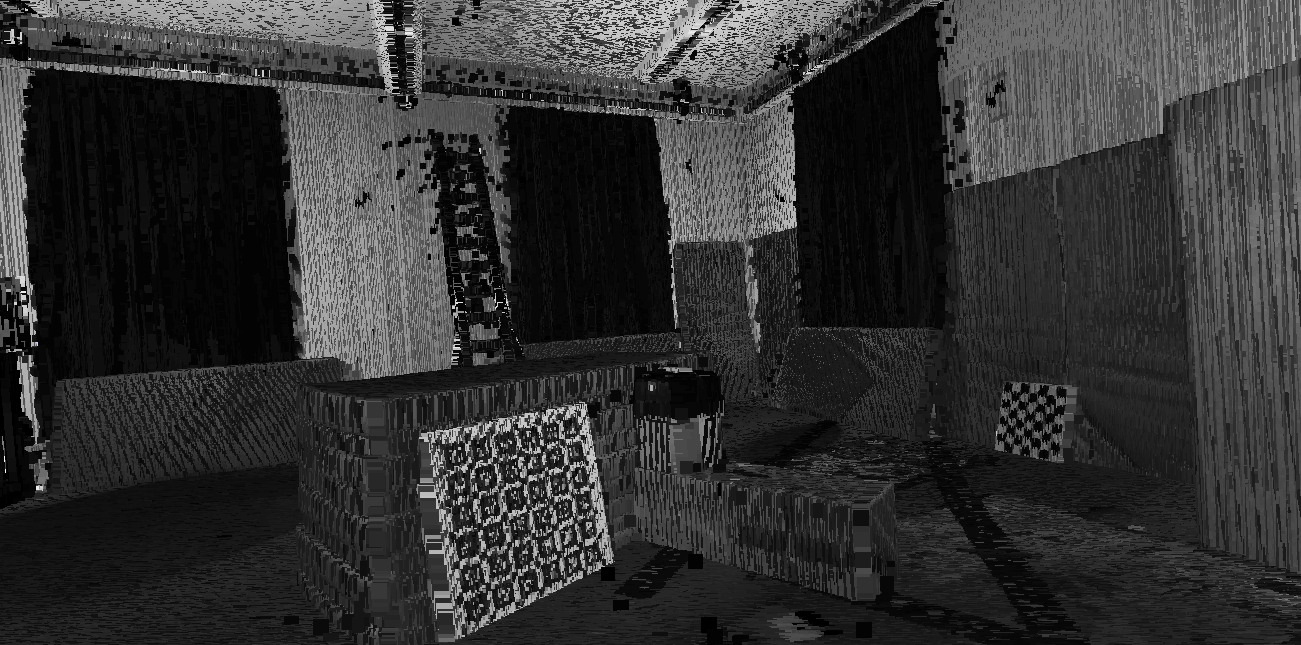
\includegraphics[scale=0.2]{Euroc/Pointcloud2.png}
	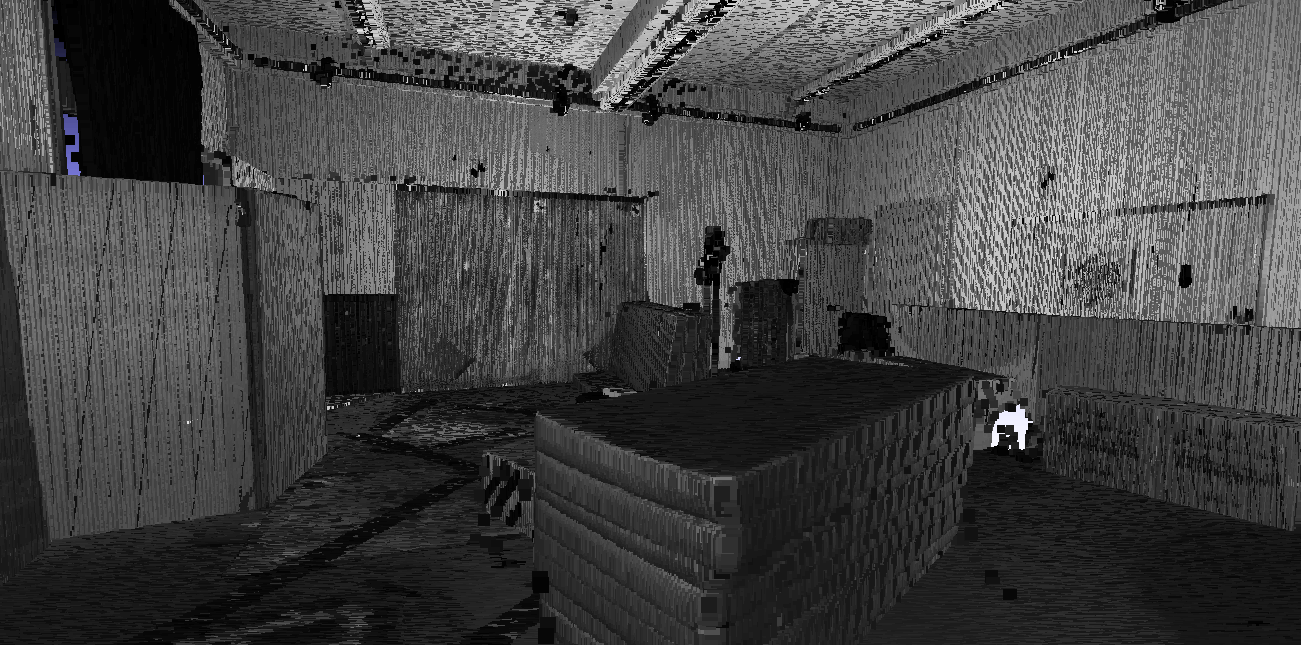
\includegraphics[scale=0.2]{Euroc/Pointcloud3.png}
	\caption{Nubes de puntos de la habitación utilizada en el EuRoC MAV Dataset}
	\label{fig:pointcloudEuroc}
\end{figure}

.


\section{Librería de desarrollo}

\subsection{OpenCV}

\begin{wrapfigure}{R}{5cm}
	\begin{center}
		\vspace*{-0.2in}
		
\includegraphics[width=4cm]{opencv}
	\end{center}
	\caption{Logo de la librería OpenCV}
\end{wrapfigure}

Para la implementación de los módulos previamente descritos, es necesario el uso de librerías y entornos de trabajo, que permitan un manejo eficiente de las imágenes. Además, el uso de de plataformas que se encuentren estandarizadas en esta área de estudio, facilita que el desarrollo del presente trabajo siga avanzando de la mano de futuros desarrolladores. En base a esto, se seleccionó la librería OpenCV\footnote{\url{http://opencv.org/}} para la implementación de los módulos necesarios en el sistema de generación de mosaico.

OpenCV (del inglés: \textit{Open Source Computer Vision}) es una librería de procesamiento de imágenes desarrollada por la empresa Intel\footnote{\url{http://www.intel.com}} en el año 1999. Esta librería ofrece un gran numero de algoritmos optimizados (actualmente mas de 2.500), el cual proporciona un entorno de desarrollo altamente eficiente para aplicaciones de procesamiento de imágenes. Asimismo presenta una gran aceptación por parte de los usuarios en el mundo académico y comercial, con mas de 47 mil usuarios activos, y un numero de descargas que supera los 14 millones. Se considera el estándar de facto en la comunidad de desarrolladores, y en especial para proyectos de investigación en procesamiento de imágenes y visión por computadora. 

Esta plataforma tiene soporte para distintos sistemas operativos, como \textit{Windows, Linux, Mac OS, iOS y Android.} Además de tener la posibilidad de trabajarla con diversos lenguajes de programación como: C++, Python, JavaScript. La motivación del presente trabajo se encuentra orientada al desarrollo de una aplicación que en un futuro pueda ser embebida en un sistema de navegación automático, con lo cual el soporte de un lenguaje de bajo nivel como C++, puede permitir el desarrollo de un algoritmo con suficiente velocidad de cómputo para este fin.

Por otra parte, esta librería presenta soporte para trabajar con la arquitectura de cálculo paralelo \textit{CUDA} (del inglés: \textit{Compute Unified Device Architecture}) de la empresa NVIDIA\footnote{\url{http://www.nvidia.com}}, con la cual se puede aprovechar el uso de las unidades de procesamiento gráfico para acelerar el rendimiento del algoritmo que se implemente. Cabe destacar que los equipos presentes en el laboratorio del \textit{GIDM} tienen disponible tarjetas gráficas con este soporte.


	\chapter{Marco Teórico}
\label{capitulo3}
\lhead{Capítulo 3. \emph{Marco Teórico}}


\section{Introducción}

En esta sección se presentarán las bases teóricas que sustentan la implementación realizada en este trabajo. Se definirá el modelo de cámara utilizado, las transformaciones de cuerpo rígido, los detectores y descriptores de características, la extracción y filtrado de correspondencias, y los filtros de fusión inercial.


\section{Modelo pinhole de la cámara}
El modelo pinhole o de pequeña apertura de la cámara es una aproximación proyectiva en la que la medición tomada por la cámara (imagen) es el resultado de una transformación del espacio en tres dimensiones del mundo  al espacio en dos dimensiones de una imagen (${\rm I\!R}^3 \to {\rm I\!R}^2$). Este modelo de cámara es el modelo más simple y utilizado en las aplicaciones de odometría y SLAM visual.

La figura  \ref{imagen:modelo_pinhole}  presenta esta aproximación. En primer lugar se observa el sistema de referencia de la cámara el cual es presentado con los ejes $X_{c}$, $Y_{c}$ y $Z_{c}$. El eje $Z_{c}$ también es conocido como el eje óptico o principal de la cámara. Además, se presenta el plano de la imagen en la figuras \ref{imagen:modelo_pinhole} y \ref{imagen:modelo_pinhole2}, el cual es un plano que se encuentra ubicado en $z= f$, donde $f$ es la distancia focal de la cámara en unidades de píxeles. En dicho plano se puede observar el sistema de referencia de la imagen, el cual se representa con los ejes punteados $u$ y $v$. En la figura \ref{imagen:coordenadas_imagen} se puede apreciar este sistema de referencia y su correspondencia con la imagen.

Cabe destacar que el sistema de coordenadas de la imagen tiene como unidad el píxel, al igual que los ejes $x$ y $y$ del plano de la imagen, los cuales tienen la misma dirección que los ejes $X_{c}$ y $Y_{c}$ .


\begin{figure}[H]
	\centering
	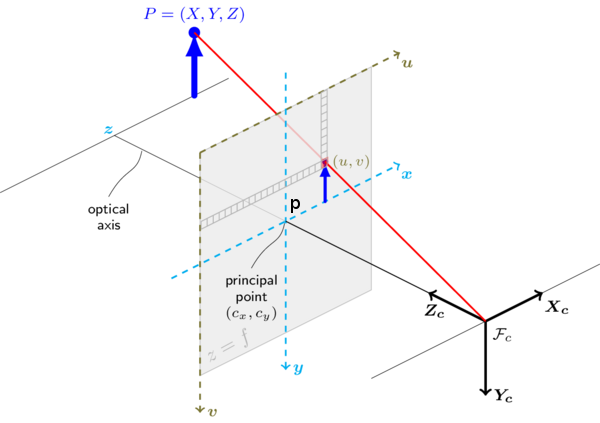
\includegraphics[width=0.7\textwidth]{modelo_pinhole}
	\caption[Modelo de apertura pequeña de la cámara]{Modelo de  pequeña apertura de la cámara\protect\footnotemark.}
	\label{imagen:modelo_pinhole}
\end{figure}
\footnotetext{\url{https://docs.opencv.org/2.4/modules/calib3d/doc/camera_calibration_and_3d_reconstruction.html}}

\begin{figure}[H]
	\centering
	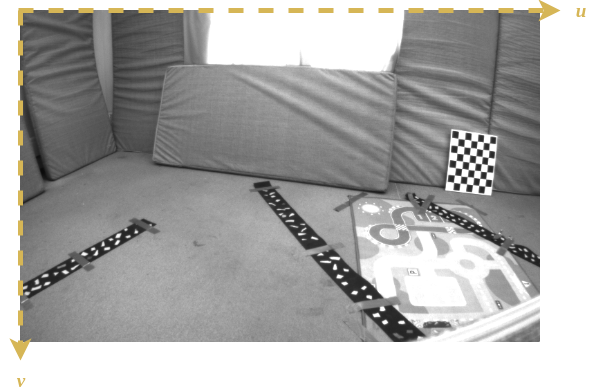
\includegraphics[width=0.7\textwidth]{coordenadas_imagen}
	\caption[Coordenadas de la imágen.]{Coordenadas de la imagen.}
	\label{imagen:coordenadas_imagen}
\end{figure}



\begin{figure}[H]
	\centering
	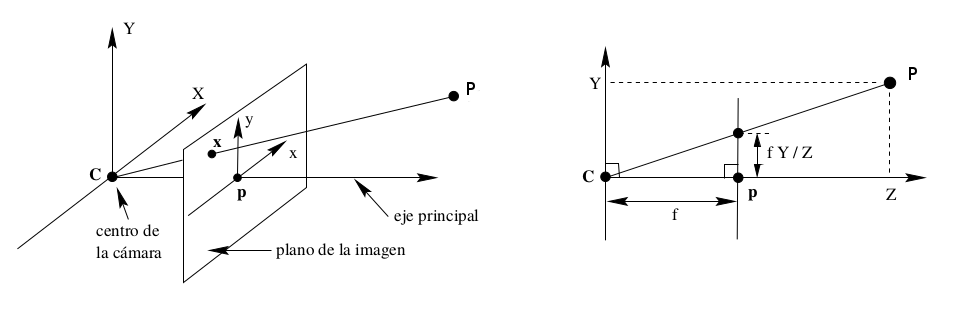
\includegraphics[width=0.7\textwidth]{modelo_pinhole2}
	\caption[Esquema de apertura pequeña de la cámara]{Esquema de apertura pequeña de la cámara. Adaptado \protect\footnotemark.}
	\label{imagen:modelo_pinhole2}
\end{figure}
\footnotetext{\url{https://www.researchgate.net/figure/Schematic-view-of-a-pinhole-camera-The-image-plane-is-shown-in-front-of-the-camera_fig2_265190953}}

El sistema de referencia de la imagen se relaciona con los ejes $X_{c}$ y  $Y_{c}$ mediante el punto principal de la imagen p = $(cx, cy , f)$ , el cual  se encuentra referenciado al sistema de la cámara. Los parámetros $cx$ y $cy$ son conocidos como el centro de la imagen y sus unidades están en píxeles. 


Finalmente, la cámara realiza una medida proyectiva del punto $P = (X, Y, Z)$ en el plano de la imagen. 
Este punto es transformado de las coordenadas en ${\rm I\!R}^3$ del mundo a las coordenadas en ${\rm I\!R}^2$ de la imagen mediante:

\begin{equation}
\begin{matrix} \left[ \begin{matrix} u \\ v \end{matrix} \right] =\left[ \begin{matrix} \frac { X.{ f } }{ Z } +{ c }_{ x } \\ \frac { Y.{ f } }{ Z } \quad +{ c }_{ y } \end{matrix} \right]  \end{matrix}
\label{eq:ProyeccionCAMSimple}
\end{equation}



En este modelo también se puede considerar que pueden existir diferentes distancias focales $f_{x}$ y $f_{y}$  en los ejes $x$ y $y$ de las coordenadas de la imagen.  Finalmente la proyección del punto P en las coordenadas de la imagen viene dada por el píxel de coordenadas $(u, v)$ mediante:

\begin{equation}
\left[ \begin{matrix} u \\ v \end{matrix} \right] =\left[ \begin{matrix} \frac { X.{ f }_{ x } }{ Z } +{ c }_{ x } \\ \frac { Y.{ f }_{ y } }{ Z } \quad +{ c }_{ y } \end{matrix} \right] 
\label{eq:ProyeccionCAM} 
\end{equation}

La ecuación \ref{eq:ProyeccionCAM} representa en el modelo de apertura pequeña la proyección que efectúa la cámara de un punto 3D $(X, Y, Z)$ dando como resultado el píxel $(u, v)$.

De la misma forma, la reproyección del píxel al punto , que resulta en una transformación de ${\rm I\!R}^2 \to {\rm I\!R}^3$, viene dada por:

\begin{equation}
\left[ \begin{matrix} X \\ Y \\ Z \end{matrix} \right] =\left[ \begin{matrix} \frac { u-{ c }_{ x } }{ { f }_{ x } } .Z \\ \frac { v-{ c }_{ y } }{ { f }_{ y } } .Z \\ Z \end{matrix} \right] =\quad Z.\left[ \begin{matrix} \frac { u-{ c }_{ x } }{ { f }_{ x } }  \\ \frac { v-{ c }_{ y } }{ { f }_{ y } }  \\ 1 \end{matrix} \right]  
\label{eq:ReproyeccionCAM} 
\end{equation}

Cabe destacar que el conjunto de puntos de la forma $s*(X, Y, Z)$, donde $s$ es un factor de escala o de profundidad, forman la recta de color rojo visualizada en la figura \ref{imagen:modelo_pinhole}. A estos puntos de ${\rm I\!R}^3$ le corresponde el mismo píxel de proyección sobre la imagen $(u, v)$. Esto implica que de una única imagen no es posible extraer la información de la profundidad del punto proyectado. Para ello es necesario más de una imagen y emplear métodos como los de triangulación.


%
\section{Detectores y descriptores de características}

Los puntos de interés, puntos clave, o \textit{"features"} (en español: características) como son comúnmente llamados, son regiones en una imagen que contienen patrones específicos, lo que hace que puedan ser fácilmente seguidos o ubicados en otra imagen. Tuytelaars y Mikolajczyk \cite{Tuytelaars} definen un punto característico local como \textit{``un patrón en la imagen que difiere de su vecindario directo''}. De esta forma, se considera que los puntos característicos deben proporcionar la posibilidad de ser identificados en diferentes imágenes con el objetivo de emparejarlos.

Para alcanzar este objetivo los detectores y extractores de puntos característicos deben cumplir con ciertas propiedades que les permita funcionar bajo distintas condiciones, en concreto se busca que estos algoritmos cumplan con las siguientes propiedades:

\begin{itemize}
	\item \textbf{Robustez:} El algoritmo debe ser capaz de detectar la misma ubicación del punto característico independientemente ante cambios en la escala, rotación, traslación, iluminación, transformaciones geométricas, artefactos de compresión y ruido.
	
	\item \textbf{Repetibilidad:} El algoritmo debe ser capaz de detectar el mismo punto característico de la misma escena bajo cambios en el punto de vista.
	
	\item \textbf{Exactitud:} El detector debe localizar el punto característico de manera precisa (misma ubicación de píxel). Especialmente para tareas de alineación de imágenes.
	
	\item \textbf{Generalidad:} El algoritmo debe ser capaz de detectar puntos que pueden ser usadas en distintas aplicaciones, es decir, que detecte varios tipos de características (esquinas, burbujas, etc.)
	
	\item \textbf{Eficiencia:} El algoritmo debe ser capaz de detectar puntos característicos en nuevas imágenes a gran velocidad, para soportar aplicaciones en tiempo real.
	
	\item \textbf{Cantidad:} El algoritmo debe detectar todos, o casi todos los puntos característicos presentes en la imagen. 
	
\end{itemize}



\begin{figure}[H]
	\centering
	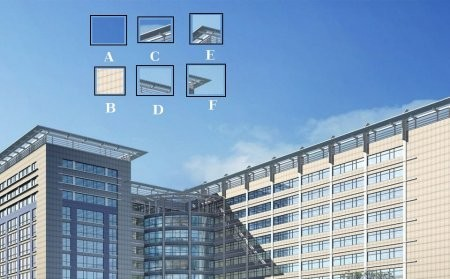
\includegraphics[width=0.7\textwidth]{features}
	\caption[Caracterización de regiones en una imagen]{Caracterización de regiones en una imagen\protect\footnotemark}
	\label{imagen:features}
\end{figure}
\footnotetext{\url{https://docs.opencv.org/3.0-beta/doc/py_tutorials/py_feature2d/py_features_meaning/py_features_meaning.html}}
%https://docs.opencv.org/3.0-beta/doc/py_tutorials/py_feature2d/py_features_meaning/py_features_meaning.html

Llegados a este punto, es necesario definir el funcionamiento de los algoritmos detectores, así como también lo que éstos consideran como puntos característicos, basados en la definición previamente planteada. Atendiendo a la imagen \ref{imagen:features}, se puede observar que se caracterizan seis áreas de interés. Analizando estos segmentos, vemos que \textbf{\textit{A}} y \textbf{\textit{B}} corresponden con superficies planas, lo que hace que sea muy difícil identificar la ubicación exacta de estas superficies en la imagen original. Por otro lado, tenemos las regiones \textbf{\textit{C}} y \textbf{\textit{D}}, las cuales corresponden con bordes en la imagen, que si bien es posible limitar en gran medida el área de búsqueda hacia toda las regiones del mismo bordes, sigue siendo difícil acertar con la ubicación correcta. Por ultimo, analizando las regiones \textbf{\textit{E}} y \textbf{\textit{F}} tenemos que corresponden a esquinas de la imagen original, en este caso se puede identificar fácilmente la ubicación exacta de la región en la imagen.

A partir de esta idea, en la cual se consideran las esquinas como regiones fácilmente identificables en una imagen, en \textit{1988} nace el primer algoritmo de detección de puntos de interés llamado Detector de esquinas de Harris \cite{harris} (nombre original en inglés: Harris Corner Detector), y como su nombre lo indica está basado en la detección de esquinas.

Retomando el concepto planteado previamente, este detector busca la diferencia de intensidad de una región con su entorno directo, es decir, se detectará una esquina para aquellas regiones que presenten una alta variación de intensidad, al desplazar la ventana estudiada en cualquier dirección. En la figura \ref{imagen:harris-window} se puede apreciar visualmente como funciona esta ventana de búsqueda.

\begin{figure}[H]
	\centering
	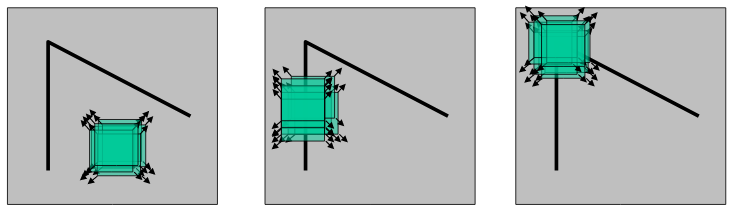
\includegraphics[width=0.9\textwidth]{harris-window}
	\caption[Ventana de búsqueda para de detección de esquinas]{Ventana de búsqueda para de detección de esquinas, adaptado de\protect\footnotemark}
	\label{imagen:harris-window}
\end{figure}
\footnotetext{\url{https://dsp.stackexchange.com/questions/14338/}}
%https://dsp.stackexchange.com/questions/14338/

Cuando se trabajan con detectores de características, se desea que estos sean invariantes ante la mayor cantidad de variables posibles, tal y como se menciona en la propiedad de robustez que deben tener estos algoritmos. Pese a que el detector presentado anteriormente es invariante ante la traslación y la rotación (ya que las esquinas se mantienen como esquinas si son rotadas o desplazadas), no funciona de la misma forma ante cambios de escala. Como se observa en la figura \ref{imagen:corner-scale}, una región considerada como esquina, se podría considerar plana si es ampliada.

\begin{figure}[H]
	\centering
	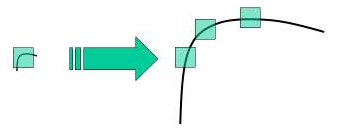
\includegraphics[width=0.85\textwidth]{corner-scale}
	\caption[Efecto del escalado sobre las esquinas]{Efecto del escalado sobre las esquinas	\protect\footnotemark}
	\label{imagen:corner-scale}
\end{figure}
\footnotetext{\url{https://docs.opencv.org/3.0-beta/doc/py_tutorials/py_feature2d/py_sift_intro/py_sift_intro.html}}
%https://docs.opencv.org/3.0-beta/doc/py_tutorials/py_feature2d/py_sift_intro/py_sift_intro.html

Con el fin de conseguir detectar los mismos puntos ante cambios en la escala de la imagen, Lindeberg, T. \cite{log} propone un algoritmo detector de ``manchas'' multi-escala a través de la búsqueda de máximos en el espacio de escala, el cual se crea utilizando un operador laplaciano. El Laplaciano de Gaussianas \textit{LoG} (del ingles: Laplacian-of-Gaussian), es una combinación lineal de segundas derivadas utilizado para detectar burbujas o manchas en una imagen. El funcionamiento es el siguiente: Dada una imagen de entrada, la representación para cada escala $-s-$ de la imagen se define como la convolución de la imagen con un filtro Gaussiano con desviación estándar $s$.

Este resultado brinda una fuerte respuesta positiva para burbujas oscuras y respuestas fuertes negativas para burbujas claras, ambas de un tamaño 2$s$, donde $s$ es la escala. De esta forma las características detectadas presentan una fuerte relación entre el tamaño de las estructuras en la imagen y el grado de difusión del filtro gaussiano. Donde la desviación estándar del filtro se usa para controlar la escala cambiando que tanto se difumina la imagen.

Una vez se haya detectado la ubicación de los puntos característicos en la imagen, la información de la localidad de éste debe ser codificada y almacenada, logrando así un descriptor único de la región con el objetivo final de ubicarlo en otra imagen. Con este fin se desarrollaron los algoritmos descriptores, los cuales una vez tengan la ubicación de los puntos característicos se encargan de convertir la información de su alrededor en una serie de números, o un vector que permita diferenciar un punto clave de otro. Esta información también es necesaria que sea invariante ante las variable mencionadas previamente, para lograr una identificación eficiente del mismo punto en distintas imágenes bajo distintas condiciones.

Partiendo de estos problemas, y del hecho que el cálculo del operador LoG es computacionalmente costoso, en \textit{2004 D. Lowe} crea el detector y descriptor \textit{SIFT} \cite{sift} (del inglés: Scale Invariant Feature Transform), en el cual el espacio de escala es construido en forma piramidal con la diferencia de gaussianas DoG (del inglés: Difference of Gaussians). En este sentido, El operador DoG ofrece una aproximación al LoG, donde el cálculo se realiza sin convolución restando niveles de escala adyacentes de una pirámide gaussiana. El proceso para la detección y descripción de puntos de interés de este algoritmo, consta de cuatro pasos principales:

El primero realiza una detección de máximos en el espacio de la escala aplicando la diferencia gaussiana \textit{DoG}. Para esto, se aplica el filtro gaussiano con distintos tamaños de media (se tienen distintas escalas), luego restando estas imágenes para distintos pares de escalas se logra la diferencia de gaussiana. Posteriormente se buscan los máximos locales a lo largo del espacio (coordenadas $x$ e $y$) para cada correspondiente escala. Este proceso de detección se puede visualizar en la figura \ref{imagen:sift-escalas}.

\begin{figure}[H]
	\centering
	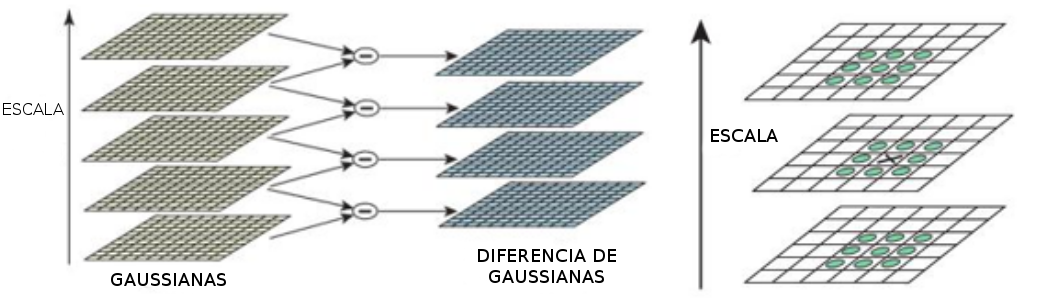
\includegraphics[width=0.85\textwidth]{sift-escalas}
	\caption[Detector SIFT]{Detección de máximos en el espacio de la escala DoG, adaptado de \cite{sift}}
	\label{imagen:sift-escalas}
\end{figure}

En segundo lugar para la localización de puntos de interés, se descartan los puntos encontrados en el paso anterior que no superen cierto valor de umbral, es decir, que no estén lo suficientemente contrastados con su entorno. Con esta etapa el algoritmo sólo toma en cuenta los puntos claves mas fuertes por cada escala. Además, con el objetivo de eliminar los bordes suficientemente contrastados que no correspondan con esquinas, el algoritmo usa una matriz Hessiana para calcular las curvaturas principales, y así quedarse solo con esquinas.

Para garantizar la invarianza con respecto a la rotación, se toman los píxeles vecinos al punto clave y se calcula la magnitud y dirección del gradiente en esa región. Con esto se hace un histograma de la magnitud del gradiente en cada dirección, donde el pico mayor del histograma indica la orientación. En el caso que exista un pico mayor al 80\% del pico principal, este se utiliza para crear otro punto de interés en la misma posición pero con la distinta rotación.

Finalmente para crear el vector descriptor por cada punto clave se crea una matriz de 16x16 alrededor de éste, dividida en 4 subregiones de 4x4 píxeles con un histograma de orientaciones para cada uno. Seguidamente, el descriptor del punto será el vector con los valores de los histogramas de las regiones 4x4 concatenados. La figura \ref{imagen:descriptor} la representación del descriptor de SIFT.

\begin{figure}[H]
	\centering
	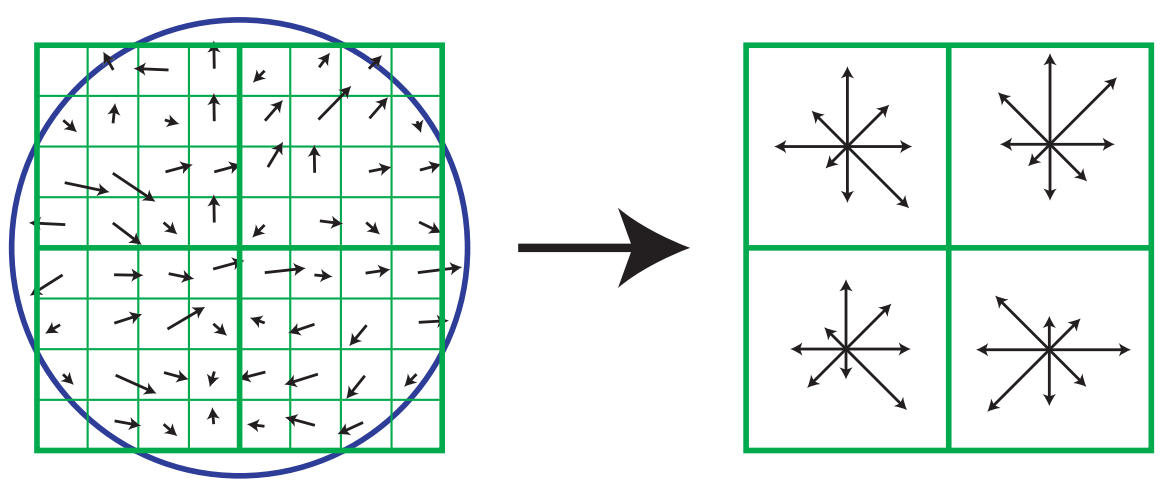
\includegraphics[width=0.7\textwidth]{sift-descriptor}
	\caption[Descriptor SIFT]{Izquierda: imagen de gradientes. Derecha: descriptor del punto clave. de \cite{sift}}
	\label{imagen:descriptor}
\end{figure}


En el año 2006, un grupo de tres personas: Bay, H., Tuytelaars, T. and Van Gool, L. desarrollan \textit{SURF} \cite{surf}, el cual es un detector y descriptor de características basado en SIFT, pero con modificaciones que aumentan su velocidad de detección. Estos cambios sacrifican un poco de rendimiento y precisión, pero sin embargo lo hace mas provechoso para aplicaciones embebidas que demanden mayor velocidad de cómputo y menor uso de recursos, como por ejemplo \textit{SLAM}. El proceso para la extracción de características por parte de este algoritmo se compone de los siguientes pasos:

Como primer paso, en lugar de aproximar el laplaciano de Gauss \textit{LoG} (del inglés: Laplacian of Gaussians) con la diferencia de Gaussianas (DoG) como lo hace SIFT, este algoritmo aproxima LoG con cuadrados para promediar la imagen. La ventaja de aplicar filtros con cuadrados es que con la ayuda de imágenes integrales el cálculo computacional se reduce en gran medida.

\begin{figure}[H]
	\centering
	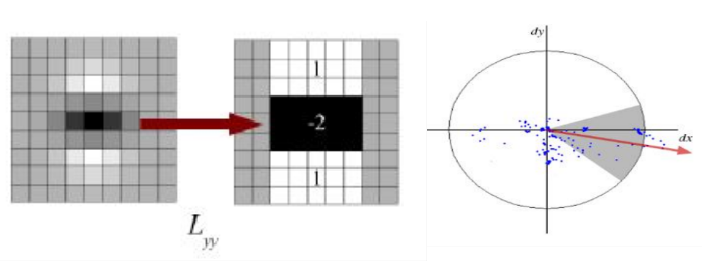
\includegraphics[width=0.8\textwidth]{surf}
	\caption[Detector y descriptor SURF]{Izquierda: aproximación a la derivada de segundo orden del filtro gaussiano (derivada parcial en el eje \textit{y}) y su aproximación con un filtro cuadrado. Derecha: vector de orientación del descriptor. Adaptado de \cite{surf}}
	\label{imagen:surf}
\end{figure}

En función de identificar la orientación, el algoritmo utiliza la respuesta Wavelet Haar en horizontal y vertical en un vecindario de 6$s$ (donde $s$ es la escala evaluada) píxeles al rededor del punto de interés, Luego estas respuestas son representadas como puntos en el espacio, para luego calcular la orientación dominante con la suma de todos los resultados dentro de una ventana deslizante de apertura 60$^\circ$. En la figura \ref{imagen:surf} se puede visualizar en el lado izquierdo, la derivada de segundo orden del filtro gaussiano, seguida de su aproximación con un filtro cuadrado. Del lado derecho se ilustra el vector de orientación en función a la distribución de puntos estudiados.

El siguiente avance importante en los algoritmos de detección aparece en el año 2011 con \textit{ORB} \cite{orb} (del inglés: Oriented FAST and Rotated BRIEF), este utiliza una combinación del detector FAST (del inglés: Features from Accelerated Segment Test) y del descriptor BRIEF (del inglés: Binary Robust Independent Elementary Features), este nuevo algoritmo se caracteriza por su alta velocidad de procesamiento manteniendo un buen rendimiento, gracias al uso de un descriptor binario. 

Como se mencionó utiliza el algoritmo FAST, el cual consiste en encontrar esquinas evaluando los píxeles en un perímetro circular, de esta forma, un punto será detectado como esquina si la cantidad de píxeles de color opuesto al evaluado, supera cierto valor de umbral (ver izquierda en la figura \ref{imagen:orb}), posteriormente con el fin de aumentar la robustez, es aplicado el algoritmo de clasificación de esquinas de $Harris$. También se realiza con una estructura piramidal evaluando varias escalas (al igual que SIFT).

\begin{figure}[H]
	\centering
	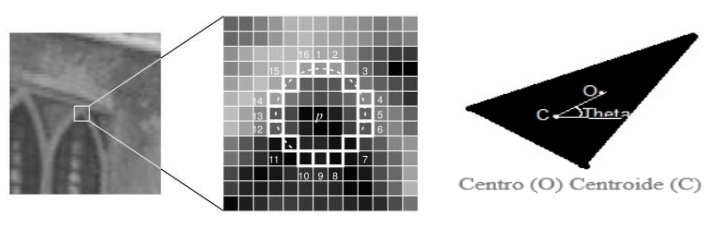
\includegraphics[width=0.9\textwidth]{orb}
	\caption[Detector y descriptor ORB]{izquierda: detección de esquinas usando FAST, de \cite{fast}. derecha: descriptor basado en BRIEF, adaptado de\protect\footnotemark }
	\label{imagen:orb}
\end{figure}

\footnotetext{\url{https://gilscvblog.com/2013/10/04/}}
Como el algoritmo FAST no toma en cuenta la orientación, en el ORB se modificó para que calculara la orientación de la siguiente forma: Se considera una región ubicada en el centro del punto estudiado, luego se calcula el centroide de la región en función a la intensidad de los puntos. De esta forma, la dirección del vector desde el punto central  hasta el centroide es asignado como vector de orientación. Observando a la derecha en la figura \ref{imagen:orb} se aprecia un ejemplo del lugar del centroide \textit{(C)} y del centro \textit{(O)} para una región en particular.

El descriptor utilizado para BRIEF es un descriptor binario y no vectorial. El mismo produce una palabra de $n$-bits usando el algoritmo \textit{Local Binay Tests} (LBT), el problema de esta representación es que no es muy robusta ante cambios en la rotación. Para resolver esto ORB utiliza la información de la orientación previamente calculada en el paso de detección para aplicar LBT en esa orientación.

Los algoritmos de detección que se mencionaron hasta este momento tienen una característica en común, y es que cuando trabajan con el esquema piramidal lo hacen bajo el espacio de escala Gaussiano, el cual es una instancia particular de difusión lineal. De esta forma, al utilizar este filtro no se respetan los limites naturales de los objetos y se difumina del mismo nivel toda la región de la imagen cuando se avanza entre niveles de escala.

Enfocándose en esta característica, en el año de \textit{2012} se desarrolla el detector y descriptor llamado KAZE \cite{kaze} por parte de \textit{Pablo Fernández Alcantarilla}. Este novedoso algoritmo opera completamente en un espacio de escala no lineal, y para ello utilizan un esquema de división de operadores aditivos (\textit{AOS}, del inglés: Additive Operator Splitting), que les permite obtener espacios de escala no lineales de forma eficiente. De este modo se puede realizar un difuminado localmente adaptativo, posibilitando que se remueva el ruido en las imágenes, manteniendo información importante sobre los bordes de los objetos al avanzar en el espacio de escala. En la figura \ref{imagen:kaze} se puede observar como afecta en los bordes de los objetos el aplicar un filtro de difusión lineal, y uno que no lo es, bajo el esquema propuesto por este algoritmo.

\begin{figure}[H]
	\centering
	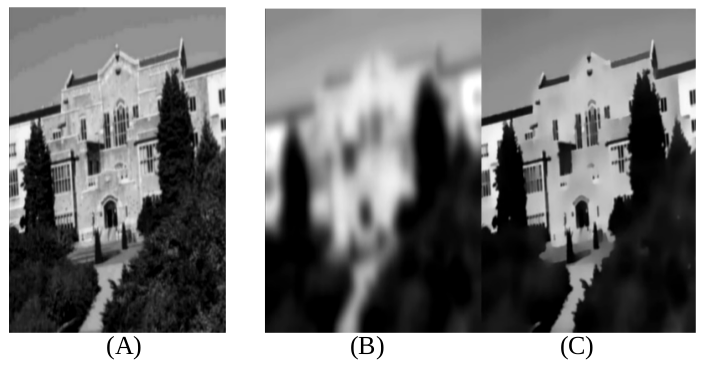
\includegraphics[width=0.85\textwidth]{kaze}
	\caption[Filtro no lineal propuesto por KAZE]{\textit{(A)}: imagen original, \textit{(B)} filtro lineal Gaussiano, \textit{(C)} filtro no lineal propuesto en KAZE, adaptada de \cite{kaze}}
	\label{imagen:kaze}
\end{figure}

Bajo este mismo esquema de difusión no lineal, el mismo autor en el año \textit{2013} desarrolla la versión acelerada de este algoritmo que recibe el nombre de \textit{A-KAZE} \cite{akaze} (del ingles: Accelerated KAZE). Esta mejora utiliza un esquema basado en difusión explícita rápida \textit{FED} (del ingles: Fast Explicit Difussion) en lugar de \textit{AOS}, el cual es un nuevo esquema piramidal que incrementa en gran medida la velocidad de cómputo para construir el espacio de escala no lineal.

Para el cálculo de la orientación el primer algoritmo \textit{KAZE} utiliza un descriptor para la orientación similar al que emplea SURF. Este encuentra la orientación dominante en un área circular de radio 6$s$ ($s$ corresponde con la escala), y para cada muestra del círculo se calcula la derivada de primer orden en las direcciones $x$ e $y$, y se ponderan con una gaussiana centrada en el punto de interés. Luego, las respuestas de estas derivadas son representadas como puntos en un espacio vectorial, donde la orientación dominante se haya sumando las respuestas dentro de un segmento de circulo deslizante con apertura de 60$^\circ$.

Por otro lado, la versión acelerada \textit{A-KAZE} emplea un descriptor basado en una versión modificada del algoritmo de diferencia local binaria \textit{LDB} \cite{ldb} (del ingles: Local Difference Binary), llamado M-LBD (del ingles: Modified Local Difference Binary), el cual aprovecha al máximo la información del espacio de escala no lineal. La modificación consiste en hacer un sub-muestreo de cada región que divide la zona del descriptor, en lugar de calcular el promedio de todos los píxeles de la región, es decir, se tienen muestras de cada subdivisión para distintas escalas.


\section{Emparejadores de puntos característicos}

En este punto ya hemos estudiado los distintos algoritmos que permiten encontrar y clasificar puntos de interés en las imágenes. Ahora bien, es necesario identificar cuales de estos puntos corresponden con la misma ubicación, tal y como podemos observar en la figura \ref*{imagen:match}. Para establecer esta relación se utilizan los algoritmos emparejadores de características, los cuales relacionan estos puntos en base a sus descriptores.

\begin{figure}[H]
	\centering
	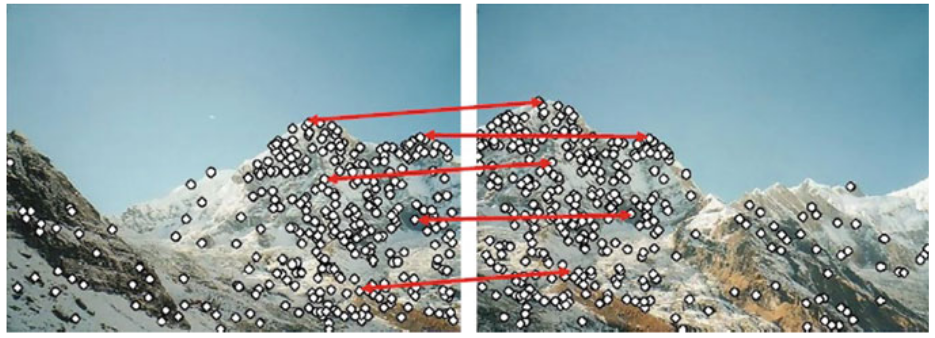
\includegraphics[width=14cm]{match}
	\caption[Emparejamiento de puntos característicos]{Emparejamiento de puntos que corresponden a la misma ubicación, de \cite{comp-vision} }
	\label{imagen:match}
\end{figure}

El proceso para realizar el emparejamiento consiste en el siguiente: Teniendo un punto característico $P_{1}$ perteneciente a la imagen $1$, y por otro lado se teniendo un punto $P_{2}$ perteneciente a la imagen $2$, Se calcula la distancia entre los descriptores $D_{1}$ y $D_{2}$. En el caso de descriptores vectoriales, esta distancia corresponde con la distancia \textit{Euclidiana}, dada por la siguiente expresión:
\begin{displaymath}
D = \sqrt{ (v_{1}-q_{1})^2 + (v_{2}-q_{2})^2 + \cdots + (v_{n}-q_{n})^2 }
\end{displaymath}
Donde $v_{n}$ corresponden con los componentes del vector descriptor $D1$, $q_{n}$ con los componentes del vector descriptor $D2$, y $n$ en el numero de componentes de ambos vectores. Por otro lado, para los descriptores binarios, se calcula la distancia \textit{Hamming}, dada por la siguiente expresión:
\begin{displaymath}
D = ||D_{1} \oplus D_{2}||
\end{displaymath}
Este proceso se repite hasta tener la distancia de cada punto de la imagen $1$ con todos los puntos de la imagen $2$, y viceversa. Al tener estas distancias, los puntos se emparejarán si y solo si se cumplen las siguientes condiciones: 

\begin{enumerate}[label=(\roman*)]
	\item El punto $P_{1}$ presenta la mejor distancia con $P_{2}$, en relación a todos los puntos de la imagen $2$.
	
	\item El punto $P_{2}$ presenta la mejor distancia con $P_{1}$ en relación a todos los puntos de la imagen $1$.
\end{enumerate}

Este proceso es mejor conocido como emparejamiento por fuerza bruta, ya que se compara entre todos los puntos por la mejor pareja posible. Aún cuando se asegura obtener el mejor emparejamiento, siendo viable para trabajar con pocos datos, el hecho de probar todas los casos posibles cuando se tiene una gran cantidad de puntos, incrementa en gran medida el tiempo de cómputo. Para efectuar este proceso de una forma eficiente se desarrollaron algoritmos basados en la búsqueda de vecinos mas cercanos. En este sentido se cuenta con el algoritmo \textit{kd-forest} (abreviado del inglés: k-dimensional forest), el cual es una mejora del algoritmo \textit{kd-tree} (abreviado del inglés: k-dimensional tree) para mejor desempeño al usar vectores multidimensionales, implementado en la librería para la rápida aproximación de vecinos mas cercanos FLANN \cite{flann} (del inglés: Fast Library for Approximate Nearest Neighbors).

%\textit{kd-tree} es una estructura de datos de segmentación de espacios para organizar puntos en un espacio de k dimensiones
\section{Módulo comparativo}

Una vez se conocen los algoritmos que se proponen utilizar, es necesario comparar su rendimiento bajo distintas condiciones, de modo que se pueda seleccionar el indicado para cada tipo de aplicación. En este sentido, se pretende estudiar el rendimiento en base a los siguientes parámetros:

\begin{itemize}
	\item \textbf{Tiempo de ejecución:} Tiempo en el que se detectan y describen las características en dos imágenes con las mismas dimensiones.
	
	\item \textbf{Cantidad de puntos detectados:} Cantidad total de puntos detectados y emparejados en dos imágenes.
	
	\item \textbf{Cantidad de puntos emparejados:} Cantidad total de puntos emparejados correctamente luego de descartar parejas erróneas. 
\end{itemize}

Adicionalmente, se propone aplicar algunos métodos que permiten aumentar el rendimiento de los algoritmos de detección, así como también implementar un proceso que permita reducir o eliminar falsos positivos al emparejar puntos de interés. 

\section{ Orientación de un cuerpo en el espacio}

La representación de la orientación de un cuerpo en el espacio puede ser expresada mediante diferentes representaciones, entre las cuáles se destacan la representación mediante ángulos de Euler,  la representación en ángulos de Roll, Pitch y Yaw (RPY), la representación en cuaterniones, y la representación  matricial mediante matrices de rotación de 3x3. Las dos primeras son más utilizadas con fines de visualización de la orientación ya que es posible graficar cada uno de los ángulos del robot para observar la variación de la orientación del robot en el tiempo, mientras que la representación en cuaterniones y matricial son formas compactas que permiten obtener la orientación final del robot mediante la concatenación de operaciones matemáticas. En particular, la representación de cuaterniones se considera más eficiente que la matricial por poseer un numero menor de operaciones mátematicas para obtener una  orientación determinada. Todas estas representaciones poseen transformaciones equivalentes para pasar de una representación a otra. En la figura \ref{imagen:rpy} se presenta el sistema de representación en RPY, el cual es utilizado en este trabajo para la visualización de la orientación y su error de estimación.


\begin{figure}[H]
	\centering
	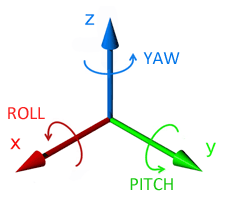
\includegraphics[scale=0.6]{RPY}
	\caption[Representación de la rotación como ángulos  RPY]{Representación de la rotación como ángulos RPY. La orientación del cuerpo se obtiene mediante la rotación de forma secuencial de los ejes de Roll, Pitch y Yaw en el sentido que se presenta en la figura.}
	\label{imagen:rpy}
\end{figure} 

En la representación RPY se puede definir cualquier rotación como la operación consecutiva de 3 rotaciones elementales:



\begin{itemize}
	\item Una rotación alrededor del eje X, definido entre ${-180}^{\circ }$ y ${180}^{\circ }$, a la que se le denomina roll o cabeceo $ \phi$. 
	\item Una rotación alrededor del eje Y, definido entre ${-90}^{\circ }$ y  ${90}^{\circ }$, a la que se le denomina pitch o alabeo $\theta$.
	\item Una rotación alrededor del eje Z, definido entre ${-180}^{\circ }$ y ${180}^{\circ }$, a la que se le denomina yaw o guiñada $\psi$.
	
	
\end{itemize}

\subsection{ Representación Matricial de la orientación }

En la representación matricial, la rotación de un cuerpo puede ser representada una matriz de 3x3:

\begin{equation}
\begin{matrix} R\quad =\quad \quad \begin{bmatrix} { r }_{ 11 } & { \quad r }_{ 12 } & { \quad r }_{ 13 } \\ { r }_{ 21 } & { \quad r }_{ 22 } & { \quad r }_{ 23 } \\ { r }_{ 31 } & { \quad r }_{ 32 } & { \quad r }_{ 33 } \end{bmatrix}\quad  \end{matrix}
\label{eq:MatrizRotacion}
\end{equation}

Esta matriz debe ser ortogonal de determinante uno:

\begin{equation}
{ R }^{ T }\quad =\quad { R }^{ -1 }
\label{eq:Propiedad1MatrizRotacion}
\end{equation}
\begin{equation}
det(R)\quad =\quad 1
\label{eq:Propiedad2MatrizRotacion}
\end{equation}


 Y  debido a estas propiedades  puede representar una función de transformación de (${\rm I\!R}^3 \to {\rm I\!R}^3$), ya que la multiplicación de una matriz rotacional con un punto perteneciente a ${\rm I\!R}^3$ genera otro punto de ${\rm I\!R}^3 $:
 
 \begin{equation}
 \begin{pmatrix} \begin{matrix} X' \\ Y' \\ Z' \end{matrix} \end{pmatrix}\quad =\quad R\quad \begin{pmatrix} \begin{matrix} X \\ Y \\ Z \end{matrix} \end{pmatrix}\quad 
 \label{eq:Propiedad3MatrizRotacion}
 \end{equation}
 
 
 También es posible obtener la orientación final de un cuerpo mediante la concatenación de matrices de rotación:
 
 
  \begin{equation}
 { R }_{ 3 }\quad =\quad { R }_{ 1 }{ R }_{ 2 }
 \label{eq:Propiedad4MatrizRotacion}
 \end{equation}
 
 Donde ${ R }_{ 1 }$ representa la orientación inicial, ${ R }_{ 2 }$ el cambio de orientación, y ${ R }_{ 3 }$ la orientación final.
 
 En la figura \ref{imagen:rpy2matriz} se presenta la forma en la que es posible obtener la matriz rotacional a partir de los ángulos RPY.
 
 \begin{figure}[H]
 	\centering
 	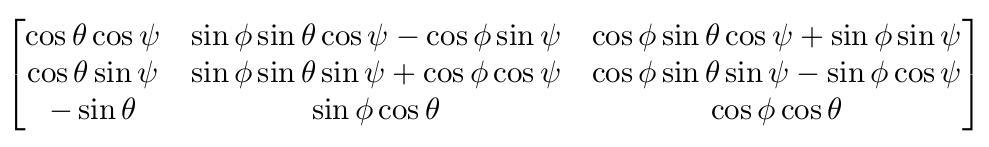
\includegraphics[scale=0.4]{RPY2Matriz}
 	\caption[Relación entre RPY y la matriz rotacional]{Relación entre RPY y la matriz rotacional. }
 	\label{imagen:rpy2matriz}
 \end{figure} 
 
 Y de forma equivalente:
 

\begin{align}
 \psi \quad =\quad \arctan { (\frac { { r }_{ 21 } }{ { r }_{ 11 } }) } 
 \\ \theta \quad =\quad \arctan { (\frac { -{ r }_{ 31 } }{ \sqrt { { { r }_{ 32 } }^{ 2 }\quad +\quad { { r }_{ 33 } }^{ 2 } }  } ) } \quad 
 \\ \phi \quad =\quad \arctan { (\frac { { r }_{ 32 } }{ { r }_{ 33 } } ) } \quad 
 \label{eq:Matriz2RPY}
 \end{align}

\section{ Transformaciones de cuerpo rígido }

El movimiento de un robot en el espacio puede ser descrito mediante un movimiento rotacional y un movimiento traslacional. Una transformación de cuerpo rígido representa el cambio de movimiento rotacional y traslacional de un cuerpo respecto a otro sistema de referencia.

En aplicaciones de odometría y SLAM, las transformaciones de cuerpo rígido son utilizadas debido a que se asume que el entorno del robot se encuentra fijo, y por lo tanto, la posición y orientación del robot puede estar vinculada a un sistema de referencia fijo. Esto permite que el robot se pueda localizar respecto a su entorno y que se pueda obtener la trayectoria del robot como una concatenación de transformaciones de cuerpo rígido.

Considerar que partes del entorno se pueden movilizar aumenta en gran medida la complejidad de la estimación del movimiento del robot.

En síntesis, una transformación de cuerpo rígido $T$  es una matriz de 4x4 constituida por una matriz de rotación $R$ y un vector de traslación $t = {(tx, ty, tz)}^{T}$:

\begin{equation}
\begin{matrix} { { T } }\quad =\quad \begin{bmatrix} R & \quad { { t } } \\ { 0 }^{ T } & \quad 1 \end{bmatrix}\quad  \end{matrix}\quad =\quad \begin{bmatrix} { r }_{ 11 } & { \quad r }_{ 12 } & { \quad r }_{ 13 } & \quad t_{ x } \\ { r }_{ 21 } & { \quad r }_{ 22 } & { \quad r }_{ 23 } & { \quad t }_{ y } \\ { r }_{ 31 } & { \quad r }_{ 32 } & { \quad r }_{ 33 } & \quad { t }_{ z } \\ 0 & 0 & 0 & 1 \end{bmatrix}
\label{eq:TC}
\end{equation}

Esta matriz tiene en total 6 grados de libertad: tres grados pertenecientes a la rotación alrededor de los ejes $x$, $y$ y $z$, y tres grados de traslación $x$, $y$ y $z$. 

La representación del vector $t$ es canónica, ya que los tres componentes del vector corresponden directamente
a tres grados de libertad. Sin embargo, la representación R de la rotación no es
canónica, ya que posee nueve parámetros, pero en conjunto solo representan
tres grados de libertad. Los seis parámetros restantes están restringidos debido
a la característica de ortogonalidad de la matriz y la necesidad de tener norma
igual a 1 para todas sus columnas y filas (propiedades \ref{eq:Propiedad1MatrizRotacion} y \ref{eq:Propiedad2MatrizRotacion}). Esto impone seis restricciones, dejando
solamente tres parámetros libres de modificación.

En este caso, los puntos de ${\rm I\!R}^3$ de la forma $P = (X, Y, Z)$  son representados por vectores homogéneos $P = {(X, Y, Z, 1)}^{T}$ , y la multiplicación de $T$ por un vector homogéneo genera otro vector homogéneo:

\begin{equation}
\begin{pmatrix} \begin{matrix} X' \\ Y' \\ Z' \end{matrix} \\ 1 \end{pmatrix}\quad =\quad T\quad \begin{pmatrix} \begin{matrix} X \\ Y \\ Z \end{matrix} \\ 1 \end{pmatrix}
\end{equation}


Las transformaciones de cuerpo rígido se utilizan para representar el movimiento traslacional y rotacional de un objeto de manera compacta y siempre están definidas en relación con un sistema de coordenadas de referencia, ya se trate del sistema de coordenadas global o de otro sistema de coordenadas arbitrario. Esto permite concatenar varias transformaciones de cuerpo rígido aplicando la multiplicación matricial entre ellas:

\begin{equation}
{ T }_{ c }\quad =\quad { T }_{ a }{ .T }_{ a-b }.{ T }_{ b-c }
\end{equation}

En este caso, tal como se ilustra en la figura \ref{imagen:TC_Concatenacion}, la orientación y posición final del cuerpo ${T}_{c}$, respecto al sistema de referencia global, es el resultado de la concatenación de la orientación y posición inicial ${T}_{a}$ en $(a)$ con el cambio de orientación y traslación ${T}_{a-b}$  de $(a)$ a $(b)$, y el cambio ${T}_{b-c}$ de $(b)$ a $(c)$.


 \begin{figure}[H]
	\centering
	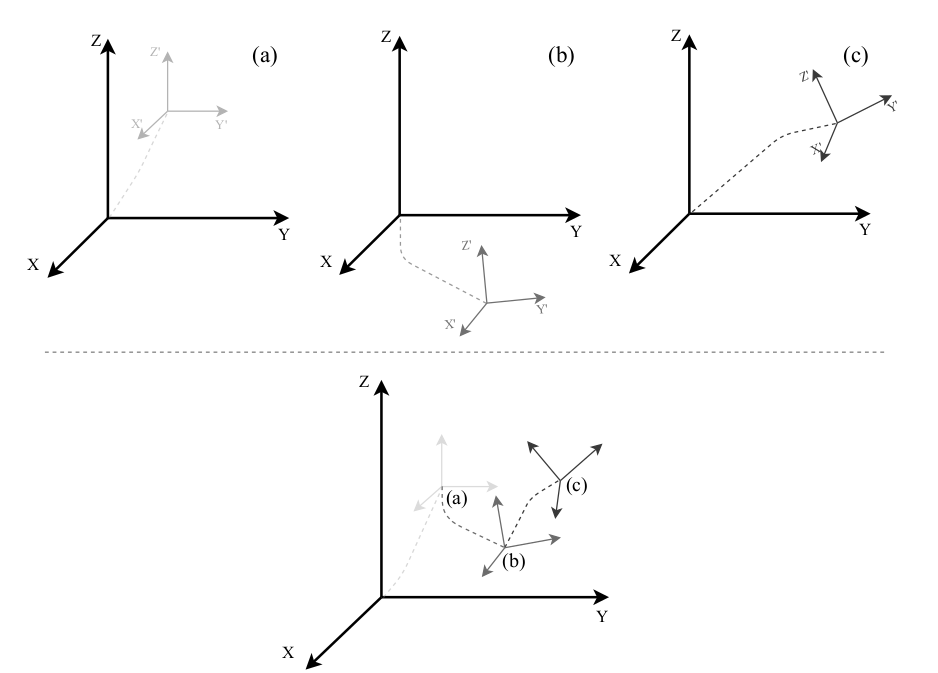
\includegraphics[scale=0.4]{TC_Concatenacion}
	\caption[Concatenación de transformaciones de cuerpo rígido]{Concatenación de transformaciones de cuerpo rígido}
	\label{imagen:TC_Concatenacion}
\end{figure} 

Las transformaciones de cuerpo rígido son fundamentales para poder relacionar las mediciones realizadas en el sistema de referencia de la imu con las imágenes tomadas por la cámara, y a su vez relacionar las estimaciones de movimiento de estos marcos de referencia con el sistema de referencia fijo.\\

La figura \ref{fig:TransformacionesRobot} presenta los sistemas de referencia presentes en el robot. La transformación ${T}_{IMU-CAM}$ relaciona los sistemas de referencia de la cámara y la imu, y corresponde a un parámetro extrínseco del sistema que es invariante debido a que la cámara y la imu se encuentran físicamente acoplados.Esta transformación se obtiene mediante la calibración de los sensores y esta conformada por dos partes: rotación del sistema de referencia de la cámara respecto al sistema de referencia de la imu; y traslación del sistema de referencia de la cámara respecto al sistema de referencia de la imu. Determinar estos parámetros con precisión es de vital importancia en los sistemas visuales-inerciales debido a que los errores de calibración puede generar resultados insatisfactorios en los algoritmos de estimación.



\begin{figure}[H]
	\centering
	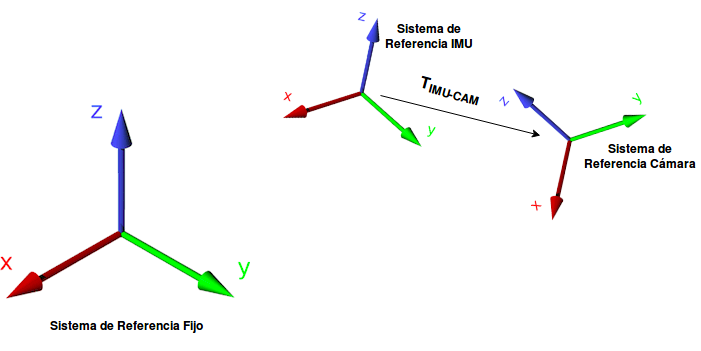
\includegraphics[scale=0.4]{ImuCam}
	\caption{Sistemas de Referencia del Robot }
	\label{fig:TransformacionesRobot}
\end{figure}


De forma concreta:

\begin{equation}
{ { T } }_{ IMU -CAM }\quad =\quad \begin{bmatrix} R_{ IMU - CAM } & \quad { { P } }_{ IMU - CAM } \\ { 0 }^{ T } & \quad 1 \end{bmatrix}\quad =\quad \begin{bmatrix} { r }_{ 11 } & { \quad r }_{ 12 } & { \quad r }_{ 13 } & \quad t_{ x-IMU } \\ { r }_{ 21 } & { \quad r }_{ 22 } & { \quad r }_{ 23 } & { \quad t }_{ y-IMU } \\ { r }_{ 31 } & { \quad r }_{ 32 } & { \quad r }_{ 33 } & \quad { t }_{ z-IMU } \\ 0 & 0 & 0 & 1 \end{bmatrix}\quad 
\label{eq:transformacionIMUCAM} 
\end{equation}

Donde ${R}_{IMU-CAM}$ es la matriz de rotación que al concantenarse con la orientación de la IMU, se obtiene la orientación de la cámara. La orientación de la IMU se representa mediante la matriz ${R}_{IMU}$, la cual es la orientación de la imu respecto al sistema de referencia fijo. En síntesis se tiene que la orientación de la cámara respecto al sistema de referencia fijo (${R}_{CAM}$) es:

\begin{equation}
{ R }_{ CAM }\quad =\quad { R }_{ IMU }*{ R }_{ IMU-CAM }\quad 
\label{eq:rotacionIMUCAM} 
\end{equation}


\section{Geometría epipolar y triangulación}

La geometría epipolar relaciona la localización en un par de imágenes de un punto $X$ en el espacio, y está relacionada directamente con la matriz esencial $E$, la cual a su vez es utilizada en métodos de estimación de la traslación y rotación basados en puntos característicos y en métodos de triangulación.

En primer lugar, se observa la figura \ref{imagen:epipolar}. En esta figura se observan la imagen 1 y la imagen 2, cuyos origines del sistema de referencia de la cámara se denotan como $O$ y $O'$, respectivamente.

El punto $X$ es proyectado en la imagen 1 en $x$. Podemos que también cada punto perteneciente a la recta $OX$ es proyectado al mismo punto $x$. Al considerar la imagen 2, se observa que la proyección del punto $X$ sobre la imagen es $x'$, pero que la posición en el plano de la imagen varia al cambiar la profundidad del punto $X$, es decir, al tomar otro punto en la recta $OX$.  Por tanto, la triangulación consiste en encontrar la profundidad correcta de $X$, conociendo las ubicaciones de sus proyecciones en un par de imágenes diferentes.

Las proyecciones de la recta $OX$ forma la linea sobre la imagen de la derecha, llamada epilinea. Se denomina epilinea del punto $x$ debido a que para encontrar este punto en la imagen 2 se debe buscar a lo largo de esta linea. Esto añade eficiencia computacional ya que no debemos buscar en la imagen entera, y a esta restricción se denomina restricción epipolar. El plano $XOO'$ es conocido como el plano epipolar.

\begin{figure}[H]
	\centering
	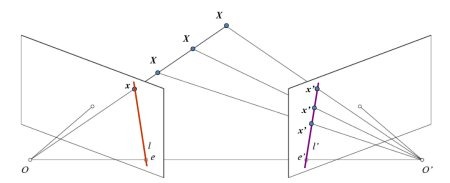
\includegraphics[width=0.7\textwidth]{epipolar}
	\caption[Geometría epipolar]{Geometría epipolar. Adaptado \protect\footnotemark.}
	\label{imagen:epipolar}
\end{figure}
\footnotetext{\url{https://docs.opencv.org/3.1.0/da/de9/tutorial_py_epipolar_geometry.html}}

También es posible calcular el vector normal al plano epipolar utilizando los vectores paralelos a las rectas $OX$ y $O'X$. Para ello, se utilizan los segmentos de recta $Ox$ y $O'x'$, y se definen los vectores de características unitarios como:

\begin{equation}
\overset { \rightarrow  }{ { f }_{ i } } =\quad \left[ \begin{matrix} \frac { u_{ i }-{ c }_{ x } }{ { f }_{ x } }  \\ \frac { { v }_{ i }-{ c }_{ y } }{ { f }_{ y } }  \\ 1 \end{matrix} \right] 
\end{equation}

Este vector unitario puede ser entendido observando la ecuación \ref{eq:ReproyeccionCAM} como un vector que no posee unidades y que apunta desde el origen de coordenadas de la cámara a la ubicación del punto $X$ en el espacio. El vector ${ f }_{ 1}$ se obtiene a partir  de $x = (u1,v1)$  y de los parámetros intrínsecos de la cámara $fx, fy, cx$ y $cy$.

De esta forma es posible visualizar que el vector normal al plano epipolar puede ser obtenido con el producto vectorial de ${ f }_{ 1}$ y ${ f }_{ 2}$. Sin embargo, estos vectores no se encuentran referenciados a un único sistema de la cámara. El vector ${ f }_{ 1}$ se encuentra calculado en el sistema $O$ y el vector ${ f }_{ 2}$ al sistema $O'$. 

Por tanto colocamos el sistema de la imagen 1 como el sistema de referencia global, y calculamos  ${ f }_{ 2}$ 
conociendo la transformación de cuerpo rígido que existe de la imagen 1 a la imagen 2:

\begin{equation}
\begin{matrix} \overset { \rightarrow  }{ { f }_{ 2,\quad 1 } } \quad =\quad { R }_{ 1 }^{ 2 }.\overset { \rightarrow  }{ { f }_{ 2 } } +{ P }_{ 1 }^{ 2 } \end{matrix}
\end{equation}

Donde $\overset { \rightarrow  }{ { f }_{ 2,\quad 1 } } \quad $ significa el vector $\overset { \rightarrow  }{ { f }_{ 2 } } $ respecto al sistema de referencia de la imagen 1.

Sin embargo, debido a que sólo es necesaria la dirección de los vectores para el calculo del vector normal, y considerando que la traslación de los sistemas ${ P }_{ 1 }^{ 2 }$ no varia la dirección del vector $\overset { \rightarrow  }{ { f }_{ 2,\quad 1 } }$, el vector normal al plano epipolar puede ser calculado como:


\begin{equation}
\overset { \rightarrow  }{ n } \quad =\quad \overset { \rightarrow  }{ { f }_{ 1 } } \quad \times \quad (\quad \overset { \rightarrow  }{ { { R }_{ 1 }^{ 2 } } } \quad .\quad \overset { \rightarrow  }{ { f }_{ 2 } } \quad )
\label{eq:normalEpipolar}
\end{equation}


%Enlazar con ecuación de Z*vector
\section{ Filtros de fusión inercial }

Existen varias alternativas para determinar la orientación de un robot a partir de las medidas del acelerómetro y el giroscópio. Entre los más conocidos se encuentran el filtro Kalman, el filtro de Madgwick, el filtro complementario de Valenti, y el filtro de Mahony.

\subsubsection{Cálculo de Roll, Pitch y Yaw}
Lá forma básica de cálculo de los ángulos de roll, pitch y yaw es mediante el cálculo de la integral numérica de sus tasas de cambio como se muestra en
la integral definida en la ecuación 
\ref{eq:integracionAnguloDefinida} o en su integral numérica de la ecuación \ref{eq:integracionAnguloNumerica}.\\

\begin{equation} \label{eq:integracionAnguloDefinida}
\phi ({ t }_{ 1 })\quad =\int _{ { t }_{ 0 } }^{ { t }_{ 1 } }{ { \omega  }_{ \phi  }dt } \quad +\phi ({ t }_{ 0 })
\end{equation}

\begin{equation} \label{eq:integracionAnguloNumerica}
{ t }_{ 1 }\quad ={ { t }_{ 0 }+T*n) })\quad =\sum _{ p\quad =\quad k }^{ k+n-1 }{ \omega _{ \phi  }(p)T } \quad +\phi ({ t }_{ 0 })
\end{equation}

Donde:\\
$t_0 $: Tiempo inicial.\\
$t_1 $: Tiempo final (en el que se tomó la ultima medida de $\omega _{ \phi  }$).\\
$\phi ({ t }_{ 0 })$: Ángulo inicial.\\
$\phi ({ t }_{ 1 })$: Ángulo que se desea estimar.\\
$\omega _{ \phi  }$: Velocidad angular.\\
$T$: Periodo de muestreo de las medidas de velocidad angular.\\
$n$: Número de medidas de $\omega _{ \phi  }$.\\
$k$: k-ésima medida de $\omega _{ \phi  }$. \\


Debido a que el giroscopio mide la velocidad angular en cada eje de rotación respecto al sistema de referencia de la IMU, cada medida debe ser transformada a un marco de referencia fijo. Por lo tanto, en la aproximación básica de orientación se determina los valores de pitch y roll ($\phi$ y $\theta$) de la orientación del robot respecto al sistema fijo en el cual la gravedad es paralela al eje $z$ a partir de las medidas del acelerómetro y luego se obtienen las tasas de cambio de los ángulos de roll, pitch y yaw a través de la transformación de la ecuación \ref{eq:transformacionVelocidadAngular}.\\

\begin{equation}
\left[ \begin{matrix} \dot { \phi  }  \\ \dot { \theta  }  \\ \dot { \psi  }  \end{matrix} \right] =\left[ \begin{matrix} 1 & \quad \quad s(\phi )t(\theta ) & \quad c(\phi )t(\theta ) \\ 0 & c(\phi ) & -s(\phi ) \\ 0 & \frac { s(\phi ) }{ c(\theta ) }  & \frac { c(\phi ) }{ c(\theta ) }  \end{matrix} \right] \left[ \begin{matrix} { \omega  }_{ x } \\ { \omega  }_{ y } \\ { \omega  }_{ z } \end{matrix} \right] 
\label{eq:transformacionVelocidadAngular} 
\end{equation}

De esta forma se pueden obtener los ángulos de orientación integrando las velocidades angulares mediante la ecuación \ref{eq:integracionAnguloNumerica}. Sin embargo, debido a los bias del giroscopio, se propagaran errores de integración a medida que se incrementa el tiempo. Por tanto, se utilizan filtros de fusión que toman en cuanta tanto la estimación de los ángulos de roll y pitch provenientes del acelerómetro, como las tasas de cambio que se pueden obtener del roll, pitch y yaw  utilizando el giroscopio mediante la ecuación \ref{eq:transformacionVelocidadAngular}.\\

En el filtro Kalman por ejemplo, se utilizan
las observaciones de la variable a estimar y de su variación respecto al tiempo, para mejorar la estimación final. Esto ocurre debido a que las estimaciones de los ángulos de roll, pitch y yaw a partir del acelerómetro y el magnetómetro sufren de errores debido al ruido y bias inherentes a las unidades de medición inercial basadas en MEMS. Lo mismo ocurre con las medidas provenientes del giroscopio. Un filtro Kalman como el de la figura  \ref{fig:diagramaFiltroKalman} toma en cuenta estas medidas y sus errores para tener una mejor estimación de la orientación del robot.\\

Cabe destacar que las unidades de medición inercial más económicas no disponen de magnetómetro, por lo el cálculo  del ángulo de yaw se ve restringido a ser obtenido sólo a partir de la integración de su tasa de cambio, lo que conlleva a que cualquier filtro de fusión inercial sufra de drift  en el tiempo de este ángulo.


\begin{figure}[H]
	\centering
	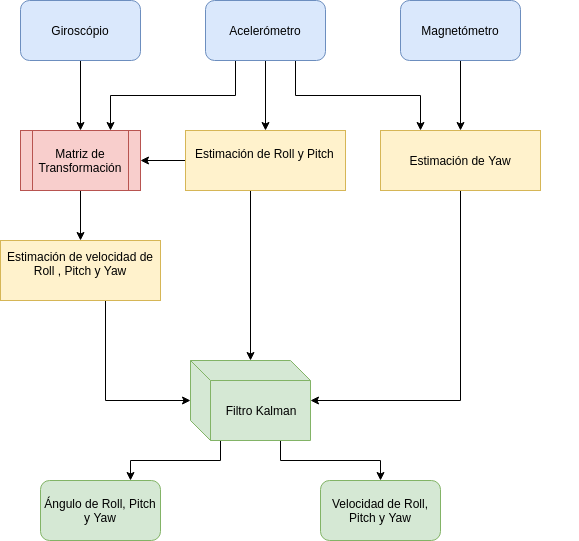
\includegraphics[scale=0.4]{FiltroKalman}
	\caption{Diagrama básico del Filtro Kalman}
	\label{fig:diagramaFiltroKalman}
\end{figure}



Sin embargo, la represetanción de la transformación presentada en \ref{eq:transformacionVelocidadAngular} presenta singularidades debido a la representación basada en cosenos directores. Es por ello que filtros como el de Madgwick y el complementario utilizan cuaterniones en la estimación de la orientación.

\subsection{ Filtro de Madgwick }

Este algoritmo fue desarrollado por Sebastián Madgwick \cite{Madgwick} y utiliza la representación de la orientación basada en cuaterniones. Este filtro utiliza el algoritmo del gradiente descendente para calcular la dirección del error de medición a partir de los datos del giroscopio.\\

El filtro de Madgwick se encuentra dividido en cuator partes: el cálculo de la orientación a partir de las velocidades angulares medidas por el giroscopio; el calculo de las orientaciones a partir de los vectores medidos del campo gravitacional y del campo magnético; la fusión de las dos estimaciones anteriores, y finalmente la normalización del cuaternion de fusión resultante. Cuando no se tiene magnetómetro sólo son fusionados las medidas de aceleración y velocidad angular.

\subsection{ Filtro complementario }
Este filtro también utiliza la representación en cuaterniones. Fusiona la estimación del cuaternion de orientación con el delta de cuaternion obtenido del acelerómetro. Este último sirve sólo como corrección de las componentes de roll y pitch, estimando el ángulo de yaw a partir de las mediciones del giroscopio. Si se provee medidas del magnetómetro, se estima otro delta de cuaternion mediante las lecturas del campo  magnético, el cual se utiliza para las correcciones de la estimación del yaw.\\

El termino de filtro complemenetario se debe al uso del analisis en el domino de la frecuencia de las señales para tener una mejor estimación de una cantidad en particular. Si se tienen señales afectadas por  ruidos de diferentes frecuencias, se utilizan dos filtros con un ancho de banda apropiado. Para estimación de la orientación de las medidas de la IMU, un filtro complementario utiliza un filtro pasa altas para la orientación estimada del giroscopio, la cual es afectada por  ruido de baja frecuencia , y un filtro pasa bajo para las medidas del acelerómetro, las cuales poseen rudio de alta frecuencia. Idealmente, la fusión de los dos filtros genera un filtro pasa todo con medidas libres de ruido. El termino complementeario deriva debido a que la frecuencia de corte es la misma para ambos filtros. \\



\subsection{Metodología}

El proceso planteado para la comparación consiste en evaluar los parámetros antes mencionados para todas las combinaciones de extractores y emparejadores que se tienen, tal y como se ilustra en la figura \ref{imagen:comparacion}.

\begin{figure}[H]
	\centering
	\includegraphics[width=14cm]{comparacion.pdf}
	\caption[Combinación de algoritmos para el analisis de rendimiento]{Combinaciones posibles del módulo comparativo}
	\label{imagen:comparacion}
\end{figure}

Cuando se utiliza un algoritmo para emparejar características, es muy común que existan parejas erróneas, puesto que al tener una gran cantidad de datos, varios pares de descriptores pueden tener la similitud necesaria para ser considerados como el mismo punto. Por esta razón es importante emplear una etapa que permita filtrar dichas parejas. Como ya se mencionó, se tienen distintos tipos de emparejadores, y en función a cada uno es necesario realizar el descarte de manera distinta. A continuación se describe el proceso asociado a cada caso.

En el caso del algoritmo de fuerza bruta: Se obtiene la distancia de la mejor pareja, luego se descartan todas las parejas cuya distancia sea mayor que la mejor obtenida multiplicada por un factor de umbral. El proceso planteado se muestra en el algoritmo \ref{fuerzabruta}.

\begin{figure}[h]
	\centering
	\begin{minipage}{.7\linewidth}
		\begin{algorithm}[H] %or another one check
			\caption{Selección de buenas parejas - Fuerza bruta}
			\label{fuerzabruta}
			\SetAlgoLined
			$P{i}$ $\equiv$  $i$-ésima pareja\\
			$D_{i}$ $\equiv$ Distancia de la $i$-ésima pareja\\
			$N$ $\equiv$ Número de puntos emparejados\\
			$U$ $\equiv$ Umbral para descartar erróneos\\
			\Begin{
				$U = 0.8$\;
				\ForEach{i $\in$ n=1,2,$\cdots$,N}{
					\If{$D_{i} < mejorDistancia$}{
						$mejorDistancia = Dp_{i}$\;
					}
				}
				\ForEach{i $\in$ n=1,2,$\cdots$,N}{
					\If{$D_{i} > mejor distancia \cdot U$}{
						eliminar $P_{i}$\;
					}
				}
			}
		\end{algorithm}
	\end{minipage}
\end{figure}

En el caso del algoritmo bajo el esquema de vecinos mas cercanos: Se descarta cada pareja cuya distancia esté muy cercana a la distancia del vecino mas próximo. El proceso planteado se muestra en el algoritmo \ref{vecinosmascercanos}.

\begin{figure}[h]
	\centering
	\begin{minipage}{.75\linewidth}
		\begin{algorithm}[H] %or another one check
			\caption{Selección de buenas parejas - Vecinos mas cercanos}
			\label{vecinosmascercanos}
			\SetAlgoLined
			$P{i}$ $\equiv$ $i$-ésima pareja\\
			$D_{i}$ $\equiv$ Distancia de la $i$-ésima pareja\\
			$V_{i}$ $\equiv$ Distancia del vecino mas cercano de la $i$-ésima pareja\\
			$N$ $\equiv$ Número de puntos emparejados\\
			$U$ $\equiv$ Umbral para descartar erróneos\\
			\Begin{
				$U = 0.5$\;
				\ForEach{i $\in$ n=1,2,$\cdots$,N}{
					\If{$D_{i} > V_{i} \cdot U$}{
						eliminar $P_{i}$\;
					}
				}
			}
		\end{algorithm}
	\end{minipage}
\end{figure}

En segundo lugar, con el objetivo de mejorar la detección se implementa una etapa de pre-procesamiento en las imágenes de entrada. Tal y como se estudió en la sección teórica, para que un punto característico sea detectado, éste debe contener información que lo diferencie de su entorno cercano, en este caso esta diferencia es medida en función a su intensidad. En base a esta definición, se propone un algoritmo que permite mejorar el contraste en la imagen mediante la técnica de estirar su histograma. De esta forma cada imagen tendrá el máximo rango de excursión sobre las intensidades de sus puntos, permitiendo que los valores de umbral al detectar regiones, se superen con más facilidad.

Es importante destacar que en proceso todas las imágenes fueron almacenadas usando variables de 8 bits, es decir, que cada valor es representado en un rango comprendido entre 0 y 255.

Para el calculo del histograma se obtiene la frecuencia de aparición de cada valor de intensidad en la imagen. Luego, se obtiene el valor de la intensidad para la cual, la cantidad de píxeles cuyo valor sea menor o igual a ésta, no supere el 1\% de la cantidad total de píxeles en la imagen, este punto es llamado percentil bajo. A continuación se repite este proceso par ubicar el percentil alto, el cual corresponde con la intensidad para la cual la cantidad de píxeles inferiores a ésta, no supera el 99\% de la cantidad total de píxeles. Al tener estos valores se aplican los siguientes criterios:

\begin{itemize}
	\item Todos los píxeles cuyo valor se encuentre por debajo del percentil bajo es igualado a 0.
	\item Todos los píxeles cuyo valor se encuentre por encima del percentil alto es igualado a 255.
	\item Todos los valores cuyo valor se encuentre entre el percentil bajo y el alto, es reescalado usando la siguiente ecuación: 
	\begin{displaymath}
		I_{pixel} = \frac{(I_{pixel} - P_{bajo}) \cdot 255}{P_{alto} - P_{bajo}}
	\end{displaymath}
\end{itemize}


%%%%%%%%%%%%%%%%%%%%%%%%%%%%%%%%%%%%%%%%%%%%%%%%%%%%%%%%%%%%%%%%%%%%%%%%%%%%%%%%%%%
\subsection{Resultados}

A continuación se presentan los resultados, para todas las combinaciones de extractores y emparejadores, bajo distintas condiciones de escena. Todas las pruebas mostradas en esta sección se realizaron utilizando un equipo con las siguientes características:  \textit{Intel\textsuperscript \textregistered } Core 2 Duo CPU E8400 @ 3.00Ghz.

En el cuadro \ref{0234} se observan los resultados para 61 pares de imágenes del fondo marino en la región de Chuspa (conjunto \textit{Chuspa}), ubicada en el estado Vargas, Venezuela. Adicionalmente, en la figura \ref{imagen:0234} se ilustran cuatro imágenes representativas del conjunto estudiado. Para esta prueba se utilizaron imágenes de $640\times480$ píxeles.

\begin{table}[h]
	\centering
	\captionof{table}{Comparación de rendimiento usando imágenes del conjunto \textit{Chuspa}}
	\label{0234}
	\renewcommand{\arraystretch}{0.8}% Tighter
	\begin{tabular}{@{}lllllll@{}}
		\toprule
			 &                				& SIFT 			& SURF & ORB 			& KAZE 				& A-KAZE \\ \midrule 
		       \hfill\vline& Total parejas  & \textbf{68679}& 32888&29637			& 6818 				& 6896   \\
		Fuerza Bruta \vline& Buenas parejas & 12601			& 3764 & 224 			& 1407 				& 520    \\
			   \hfill\vline& Precisión (\%) & 18.34			&11.44 &0.70 			&20.63 				& 7.54  \\
			   \vspace{0.3cm}
			   \hfill\vline& Tiempo (s)     & 38.27			&13.60 &\textbf{2.32}	&69.09 				& 16.99  \\
			   
			   \hfill\vline& Total parejas  & \textbf{68679}& 32888&29637			& 6818 				& 6896   \\
		FLANN  \hfill\vline& Buenas parejas &\textbf{13221} & 3895 & 282 			& 1416 				&553     \\ 
			   \hfill\vline& Precisión (\%) & 19.25			& 11.84& 0.95			& \textbf{20.76}	& 8.01 \\ 
			   \hfill\vline& Tiempo (s)     & 38.27			&13.60 &\textbf{2.32} 	&69.09 				& 16.99  \\
			   \bottomrule
	\end{tabular}
\end{table}


\begin{table}[h]
	\centering
	\captionof{table}{Comparación de rendimiento usando imágenes del conjunto \textit{Chuspa}, luego de aplicar estiramiento del histograma}
	\label{0234-2}
	\renewcommand{\arraystretch}{0.8}% Tighter
	\begin{tabular}{@{}lllllll@{}}
		\toprule
		&                				& SIFT 			& SURF & ORB 			& KAZE 				& A-KAZE \\ \midrule 
		\hfill\vline& Total parejas  & \textbf{235284}  & 98402&30500			& 59061 			& 62957   \\
		Fuerza Bruta \vline& Buenas parejas & 29200		& 7461 & 200 			& 11812 			& 3115    \\
		\hfill\vline& Precisión (\%) & 12.41			&7.58 &0.65 			&19.99 				& 4.94  \\
		\vspace{0.3cm}
		\hfill\vline& Tiempo (s)     & 113.29			&28.81 &\textbf{3.44}	&75.40 				& 21.66  \\
		
		\hfill\vline& Total parejas  & \textbf{235284}  & 98402&30500			& 59061 			& 62957   \\
		FLANN \hfill\vline& Buenas parejas &\textbf{31917}& 7461 & 257 			& 12522				& 3617     \\ 
		\hfill\vline& Precisión (\%) & 13.53			& 8.17& 0.84			& \textbf{21.20}	& 5.74 \\ 
		\hfill\vline& Tiempo (s)     & 63.81			&25.79 &\textbf{3.78} 	&75.20 				& 20.58  \\
		\bottomrule
	\end{tabular}
\end{table}




En el cuadro \ref{SR} se observan los resultados para 42 pares de imágenes. Estas imágenes fueron proporcionadas por el centro Australiano de Robótica de Campo ACFR (del inglés: Australian Center for Field Robotics) y pertenecen al conjunto de datos \textit{ScottReef 25}. Adicionalmente, en la figura \ref{imagen:SR} se ilustran cuatro imágenes representativas del conjunto estudiado. Para esta prueba se utilizaron imágenes de $640\times480$ píxeles.

%\begin{figure}{\linewidth}
\begin{table}[h]
		\centering
		\captionof{table}{Comparación de rendimiento usando imágenes submarinas del conjunto \textit{ScottReef 25}}
		\label{SR}
		\renewcommand{\arraystretch}{0.8}% Tighter
		\begin{tabular}{@{}lllllll@{}}
			\toprule
			&              	 			& SIFT 			& SURF & ORB & KAZE & A-KAZE \\ \midrule 
			\hfill\vline& Total parejas  &\textbf{100620}&48955 &21000&17952 & 19430  \\
			Fuerza Bruta \vline& Buenas parejas & 3631 			& 1383 & 55  & 1511 & 239    \\
			\hfill\vline& Precisión (\%) & 3.60			&2.82  &0.26 & 8.41& 1.23  \\
			\vspace{0.3cm}
			\hfill\vline& Tiempo (s)     & 49.87& 16.97&\textbf{5.90} &52.74 & 15.05 \\
			
			\hfill\vline& Total parejas  &\textbf{100620}&48955 &21000			&17952 			& 19430  \\
			FLANN  \hfill\vline& Buenas parejas &\textbf{3987}  & 1480 & 65  			& 1604 			&282     \\ 
			\hfill\vline& Precisión (\%) & 3.96			&3.02  &0.30			& \textbf{8.93}& 1.45  \\
			\hfill\vline& Tiempo (s)     & 36.82			& 15.70& 5.95	& 51.48			& 15.22  \\ 
			\bottomrule
		\end{tabular}
\end{table}


\begin{table}[h]
	\centering
	\captionof{table}{Comparación de rendimiento usando imágenes submarinas del conjunto \textit{ScottReef 25}, luego de aplicar estiramiento del histograma}
	\label{SR-2}
	\renewcommand{\arraystretch}{0.8}% Tighter
	\begin{tabular}{@{}lllllll@{}}
		\toprule
		&              	 			& SIFT 			 & SURF & ORB & KAZE  & A-KAZE \\ \midrule 
		\hfill\vline& Total parejas  &\textbf{231242}&115193&21000&134065 & 127859  \\
		Fuerza Bruta \vline& Buenas parejas & 5987 	& 2317 & 62  & 7621 & 796    \\
		\hfill\vline& Precisión (\%) & 2.58			&2.01  &0.29 &5.68& 0.62  \\
		\vspace{0.3cm}
		\hfill\vline& Tiempo (s)     & 125.38& 36.427& 7.08 &78.11 & 35.47 \\
		
		\hfill\vline& Total parejas  		&\textbf{231242}		&115193 &21000	&134065 		& 127859  \\
		FLANN  \hfill\vline& Buenas parejas &\textbf{6847}  		& 2542  & 65  	& 9034 			&1052     \\ 
		\hfill\vline& Precisión (\%) 		& 2.96					&2.20   &0.30	& \textbf{6.73} & 0.82  \\
		\hfill\vline& Tiempo (s)     		& 60.10					&29.59 & \textbf{7.02}	& 66.69			& 26.72  \\ 
		\bottomrule
	\end{tabular}
\end{table}
	 
\begin{figure}[h]
 	\centering
 	\vspace{0.6cm}
 	\begin{tabular}{@{}cccc@{}}
 		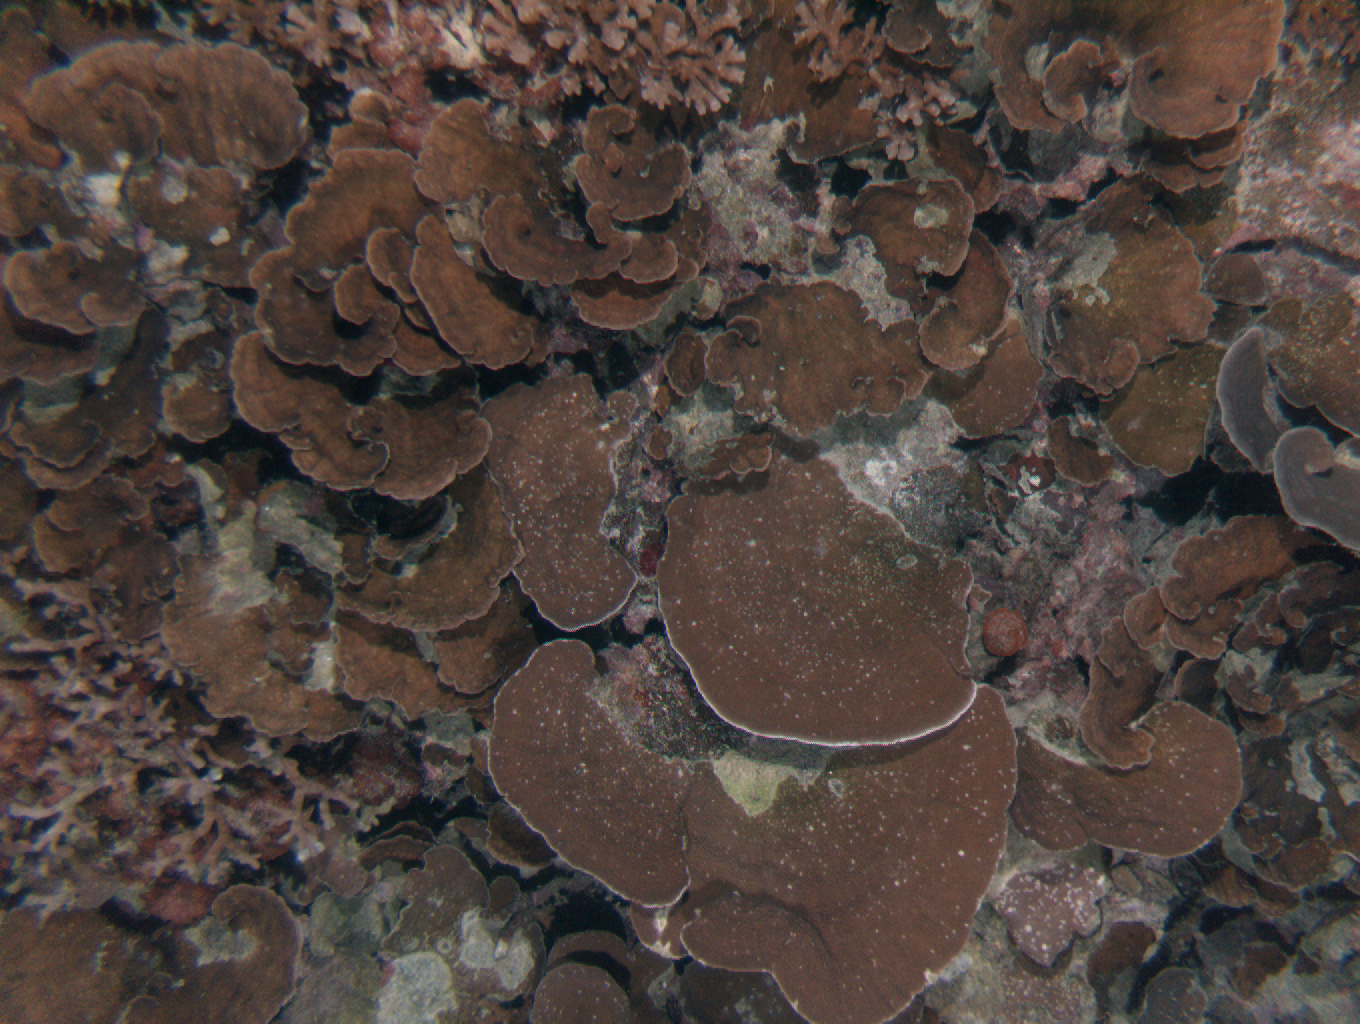
\includegraphics[width=.23\textwidth]{sr1} &
 		\includegraphics[width=.23\textwidth]{sr2} &
 		\includegraphics[width=.23\textwidth]{sr3} &
 		\includegraphics[width=.23\textwidth]{sr4} 
 	\end{tabular}
 	
 	\captionof{figure}{imágenes representativas del conjunto \textit{ScottReef 25}}
 	\label{imagen:SR}
 	
\end{figure}

En el cuadro \ref{0752} se observan los resultados para 51 pares de imágenes del fondo marino del parque nacional Mochima (conjunto \textit{Mochima}), ubicado en el estado Sucre, Venezuela. Adicionalmente, en la figura \ref{imagen:0234} se ilustran cuatro imágenes representativas del conjunto estudiado. Para esta prueba se utilizaron imágenes de $640\times480$ píxeles.

%\begin{figure}{\linewidth}
\begin{table}[h]
	\centering
	\captionof{table}{Comparación de rendimiento usando imágenes del conjunto \textit{Mochima}}
	\label{0752}
	\renewcommand{\arraystretch}{0.8}% Tighter
	\begin{tabular}{@{}lllllll@{}}
		\toprule
		&                      				& SIFT 			& SURF & ORB & KAZE & A-KAZE  \\ \midrule 
		\hfill\vline& Total parejas  &\textbf{116840}& 62472&25382&35934 & 34733   \\
		Fuerza Bruta \vline& Buenas parejas & 14659			& 6068 & 207 & 6760 & 1888    \\
		\hfill\vline& Precisión (\%) & 12.58			&9.71  &0.81 & 18.81 & 5.43  \\
		\vspace{0.3cm}
		\hfill\vline& Tiempo (s)     & 53.24			&18.37 & \textbf{2.30} &61.14 & 15.37   \\
		
		\hfill\vline& Total parejas  &\textbf{116840}& 62472&25382			&35934 				& 34733   \\
		FLANN  \hfill\vline& Buenas parejas &\textbf{15690} & 6426 & 242 			& 7175 				& 2136    \\
		\hfill\vline& Precisión (\%) & 13.42			& 5.48 &0.95  			& \textbf{19.96} 	& 6.14    \\ 
		\hfill\vline& Tiempo (s)     & 39.23			& 17.66& 2.44	& 62.07				& 15.07   \\ 
		\bottomrule
	\end{tabular}
\end{table}

\begin{table}[h]
	\centering
	\captionof{table}{Comparación de rendimiento usando imágenes del conjunto \textit{Mochima}, luego de aplicar estiramiento del histograma}
	\label{0752-2}
	\renewcommand{\arraystretch}{0.8}% Tighter
	\begin{tabular}{@{}lllllll@{}}
		\toprule
		&                      				& SIFT 			& SURF & ORB 		& KAZE 				& A-KAZE  \\ \midrule 
		\hfill\vline& Total parejas  &\textbf{146453}		& 75342&25440		&61107 				& 57797   \\
		Fuerza Bruta \vline& Buenas parejas & 16743			& 6879 & 208 		& 12105 			& 3310    \\
		\hfill\vline& Precisión (\%) & 11.43				&3.13  &0.81		& 19.80 			& 5.72  \\
		\vspace{0.3cm}
		\hfill\vline& Tiempo (s)     & 68.42				&22.05 & \textbf{2.80} &66.45       & 18.69   \\
		
		\hfill\vline& Total parejas  &\textbf{146453}& 75342&25440			&61107 				& 57797   \\
		FLANN  \hfill\vline& Buenas parejas &\textbf{18006} & 7328 & 244 			& 12890 			& 3773    \\
		\hfill\vline& Precisión (\%) & 12.29				& 9.72 &0.95  			& \textbf{21.09} 	& 6.52    \\ 
		\hfill\vline& Tiempo (s)     & 45.01				& 20.27& 2.88			& 64.77				& 17.57   \\ 
		\bottomrule
	\end{tabular}
\end{table}


\begin{table}[h]
	\centering
	\caption{Comparación de rendimiento usando imágenes del conjunto \textit{Grava}}
	\label{geotagg}
	\begin{tabular}{@{}lllllll@{}}
		\toprule
		&                      				& SIFT 			& SURF & ORB & KAZE  & A-KAZE  \\ \midrule 
			   \hfill\vline& Total parejas  &\textbf{336189}& 222251&25000&108819& 121914   \\
		Fuerza Bruta \vline& Buenas parejas & 21006			& 5853 & 126 & 10290 & 3240  \\
			   \hfill\vline& Precisión (\%) & 3.24			&2.63  & 0.5   & 9.45& 2.65  \\
				\vspace{0.3cm}
			   \hfill\vline& Tiempo (s)     & 282.76		&116.38 & 28.84 &309.29 & 92.71   \\
		
			   \hfill\vline& Total parejas  &\textbf{336189}& 222251&25000			&108819				& 121914   \\
		FLANN  \hfill\vline& Buenas parejas &\textbf{22610} & 6525 & 143			& 10861				& 3749    \\
			   \hfill\vline& Precisión (\%) & 6.72			& 2.93 &0.57  			& \textbf{9.98} 	& 3.07    \\ 
			   \hfill\vline& Tiempo (s)     & 153.12		& 90.27& \textbf{28.53}	& 299.59			& 81.52   \\ 
		\bottomrule
	\end{tabular}
\end{table}
\begin{table}[h]
	\centering
	\caption{Comparación de rendimiento usando imágenes del conjunto \textit{Grava}, luego de aplicar estiramiento del histograma}
	\label{geotagg-2}
	\begin{tabular}{@{}lllllll@{}}
		\toprule
		&                      				& SIFT 			& SURF & ORB & KAZE  & A-KAZE  \\ \midrule 
		\hfill\vline& Total parejas  &\textbf{335418}		& 221287&25000&108124& 121122   \\
		Fuerza Bruta \vline& Buenas parejas & 20943			& 5812 & 127 & 10313 & 3239  \\
		\hfill\vline& Precisión (\%) & 6.24			&2.62  & 0.58  & 9.53& 2.67  \\
		\vspace{0.3cm}
		\hfill\vline& Tiempo (s)     & 278.97		&114.86 & 29.54 &300.12 & 92.31   \\
		
		\hfill\vline& Total parejas  &\textbf{335418}& 221287&25000			&108124				& 121122   \\
		FLANN  \hfill\vline& Buenas parejas &\textbf{22555} & 6509 & 149	& 10880				& 3754    \\
		\hfill\vline& Precisión (\%) & 6.72			& 2.94 &0.59  			& \textbf{10.06} 	& 3.09   \\ 
		\hfill\vline& Tiempo (s)     & 153.71		& 88.25& \textbf{29.44}	& 294.61			& 83.68   \\ 
		\bottomrule
	\end{tabular}
\end{table}



Partiendo de los resultados previamente expuesto, analizaremos el rendimiento de todas las combinaciones estudiadas en función a los parámetros descritos al inicio de la sección.

Es evidente la inversa relación entre la cantidad de puntos detectados y el tiempo que le toma ese proceso. En función a la detección, podemos acotar que los algoritmos SIFT y KAZE presentan la mayor cantidad de parejas correctas, siendo SIFT el que permanece con el mayor numero a lo largo de todas las pruebas. Este resultado está relacionado con el uso de descriptores vectoriales, que permiten una descripción mas robusta de los puntos detectados. Además que en el caso de SIFT no se realiza ninguna aproximación para la obtención de las diferentes escalas de la imagen.

Por el contrario, aquellos algoritmos que utilizan descriptores binarios presentan un menor rendimiento en base a puntos emparejadas. Sin embargo, esta característica les permite realizar la extracción con una velocidad mucho mayor, patrón que se mantiene a lo largo de todas las pruebas.

Analizando los resultados del extractor \textit{KAZE}, aunque no ofrece la mayor cantidad de parejas correctas, presenta el mejor cociente entre parejas totales y correctas. Esto que indica un gran nivel de robustez en su descriptor, ya que un alto porcentaje de las parejas encontradas en un principio, efectivamente corresponden con el mismo punto.

Comparando el rendimiento de los emparejadores, podemos observar que para la mayoría de los casos el algoritmo FLANN aumenta la cantidad de parejas correctas, y al mismo tiempo disminuye el tiempo computacional. Para la mayoría de las pruebas no se tiene un mejora significativa en términos de tiempo, lo cual es debido a que este algoritmo ofrece mayores beneficios cuando la cantidad de parejas a estudiar es mucho mas elevada. Este punto se evidencia mayormente en los resultados del algoritmo SIFT, el cual ofrece mayor cantidad de parejas, y por lo tanto mayor conjunto de puntos a emparejar.

Por ultimo podemos destacar el importante aumento en la cantidad de parejas detectadas, para los casos en los que se aplicó el pre-procesamiento en la entrada. Como ya se mencionó, se debe al aumento en el contraste, lo que produce que la diferencia entre un punto característico y su vecindario se incremente, aumentando al mismo tiempo la posibilidad de ser detectado y luego emparejado.

% Intel Core 2 Duo CPU E8400 @ 3.00 Ghz
% 3.7 GiB RAM

\section{Resumen}

Como se explicó con detalle al inicio del presente capítulo, el proceso de establecer la relación entre las imágenes es un paso muy importante en la etapa de registro. De esta forma, la selección del algoritmo para la extracción de características, así como también la técnica que se use para establecer las correspondencias determinará la calidad final del mapa. Tal y como se presentó, se dispone de una gran cantidad de algoritmos para la extracción de características locales, así como también métodos eficientes para emparejarlos. Esta diversidad permite que se cuenten con algoritmos que se comporten de manera eficiente para cada tipo de aplicación, o en el caso de mapeo, para cada tipo de escena. 

En el presente capítulo se logró establecer una clasificación sobre los algoritmos de generación, en función a como aborden las etapas mas importantes de éste. Tomando en cuenta los distintos métodos y técnicas, se planteó un sistema que combina aquellas que presentan los mejores resultados, considerando los requerimientos del presente proyecto. Al mismo tiempo se describió el funcionamiento de todos algoritmos que se plantean implementar en el sistema, permitiendo que se puedan aplicar técnicas para mejorar el rendimiento en la extracción y emparejamiento. 

Tras los resultados mostrados, se logró evidenciar claramente la relación entre el rendimiento de cada combinación y los parámetros de tiempo y cantidad de parejas, esto permite una selección en función de los requerimientos de la aplicación. Adicionalmente, dada la modularidad del esquema planteado es posible reemplazar cualquiera de los algoritmo presentes para extraer y emparejar sin afectar el resto del proceso para la construcción del mosaico.

	\chapter{Alineación de imágenes}
\label{capitulo4}
\lhead{Capítulo 4. \emph{Alineación de imágenes}}


	\chapter{Dataset local}
\label{capitulo5}
\lhead{Capítulo 5. \emph{Dataset local}}


\section{Introducción}
El objetivo de este capítulo es explicar la elaboración de un dataset visual inercial, a través de la construcción de un robot prototipo, la adquisición de datos de odometría de los encoders del robot, de la captura de imágenes de la cámara empleada, y de la adquisición de las medidas tomadas por la IMU.


\clearpage

\section{Descripción del prototipo}

El prototipo realizado consiste en un robot diferencial inicialmente diseñado para la categoría Sumo de la VII Competencia Nacional de Robótica CCSBOTS 2018. El prototipo tiene un peso de 2.9 kg y es capaz de soportar pesos de hasta 4kg. Posee una placa de control a bajo nivel de los motores del robot, y una Raspberry Pi 3 que es utilizada para controlar el robot utilizando un mando del tipo joystick a través de la interfaz bluetooth. El robot posee además encoders en sus ruedas que permiten tener datos de odometría. Este prototipo tiene una autonomía aproximada de 1 hora. La figura \ref{imagen:Robot} muestra la configuración final del robot. 

Más información puede ser encontrada en el \href{https://github.com/Robot-Sumo/}{\underline{repositorio de desarrollo del robot}}.


\begin{figure}[H]
	\centering		\includegraphics[width=0.7\linewidth]{imagenes/prototipo/Robot}
	\caption{Prototipo final.}
	\label{imagen:Robot}
\end{figure}


\section{Diseño mecánico}


El diseño mecánico del robot está centrado en el diseño de la caja de velocidad del mismo. El modelaje 3D del robot se realizó utilizando Autocad como software de diseño y visualización del prototipo.



\subsection{Motores}

Los motores empleados en el diseño del robot fueron 4 motores con escobillas Mabuchi  C2162-60006. La figura \ref{imagen:prototipo/CajaMotores} presenta la configuración utilizada. El cuadro \ref{MabuchiDatasheet} presenta la información del motor suministrada por el fabricante y el cuadro \ref{MabuchiResultados} presenta los resultados de las mediciones realizadas al motor para la caracterización de su resistencia de armadura.

\begin{figure}[H]
	\centering
	\includegraphics[width=0.7\textwidth]{prototipo/CajaMotores}
	\caption[Motores Mabuchi empleados en el diseño del prototipo]{Componentes de Hardware del robot.}
	\label{imagen:prototipo/CajaMotores}
\end{figure}

\begin{table}[htbp]
	\caption{Datos del motor Mabuchi proveidos por el fabricante.}
	\centering
	\begin{tabular}{|l|c|}
		\hline
		\multicolumn{ 2}{|c|}{\textbf{Motor  Mabuchi Brush C2162-60006 19-24v HP}} \\ \hline
		Rating [volts] & 19 \\ \hline
		Test [volts] & 24 \\ \hline
		Stall Torque [N-cm] & 28.7 \\ \hline
		Max. Power [Watts] & 34.2 \\ \hline
		Max. Power [mili-hp] & 45.8 \\ \hline
		Duration [sec] & 30 \\ \hline
		Energy [Joules] & 1026 \\ \hline
		Weight [grams] & 224 \\ \hline
		Power/Weight [Watts/kg] & 153 \\ \hline
		Energy/Weight [Joules/kg] & 4580 \\ \hline
	\end{tabular}
	\label{MabuchiDatasheet}
\end{table}



\begin{table}[htbp]
	\caption{Resultados de mediciones realizadas al motor.}
	\centering
	\begin{tabular}{|l|c|}
		\hline
		No Load Current [Amps] & 0.15 \\ \hline
		Resistance [Ohms] & 15 \\ \hline
		Stall Current [Amps] & 1.6 \\ \hline
		No Load Speed [rpm] & 3500 \\ \hline
	\end{tabular}
	\label{MabuchiResultados}
\end{table}


Entre los datos relevantes en estos cuadros destacan la corriente del motor cuando es aplicado el máximo torque (denominada en inglés "Stall Current"), la cual es utilizada para el diseño de las protecciones y de los puntos de referencia de los drivers; el máximo torque aplicado por el motor (denominada en inglés "Stall Torque");  y  la velocidad sin carga (denominada en inglés "No Load Speed"). Estos 3 parámetros fueron  utilizados para el criterio de selección de la relación de reducción en el sistema de engranajes.

\subsection{Caja de velocidad}


El diseño de la caja de velocidad está centrado en la elección de la relación de reducción, que a su vez depende de la velocidad máxima y el torque máximo del robot. Para el cálculo del torque final${ T }_{ F }$ en función de la relación de reducción $R$ se emplea la ecuación \ref{eq:Torque}, donde el ${ T }_{ I }$ es el torque inicial del motor.


\begin{equation}
\label{eq:Torque}
{ T }_{ F }\quad =\quad { T }_{ I }.R
\end{equation}


En el caso del cálculo de la velocidad final de la rueda ${ V }_{ F }$ se emplea la ecuación \ref{eq:VelocidadFinal}, donde el ${ V }_{ I }$ es la velocidad inicial del motor.

\begin{equation}
\label{eq:VelocidadFinal}
{ V }_{ F }\quad =\quad \frac { { V }_{ I } }{ R } 
\end{equation}


El cuadro \ref{TablaPruebaEngranajes} presenta los resultados estimados  de torque máximo y velocidad máxima del robot para una relación de engranajes específica. En este caso la velocidad máxima del motor fue aproximada a 3000 rpm a pesar de que la medición sin carga fue cercana a los 3500 rpm, ya que las revoluciones sin carga bajan al presentar carga en el sistema de transferencia.

Cabe destacar que las ecuaciones \ref{eq:VelocidadFinal} y \ref{eq:Torque} presentan que el torque y la velocidad final son inversamente proporcionales, por lo que la relación de reducción se elije para el par más adecuado.

\begin{table}[htbp]
	\caption{Pruebas de diferentes relaciones de engranajes}
	\centering
	\begin{tabular}{|l|r|r|r|r|}
		\hline
		\textbf{Relación final de engranajes} & \textbf{20} & \textbf{15} & \textbf{12} & \textbf{8} \\ \hline
		Velocidad máxima del motor (rpm) & 3000 & 3000 & 3000 & 3000 \\ \hline
		Radio de la rueda (cm) & 3.74 & 3.74 & 3.74 & 3.74 \\ \hline
		Velocidad máxima de la rueda (rpm) & 150 & 200 & 250 & 375 \\ \hline
		Velocidad máxima de la rueda (rev/s) & 15.708 & 20.944 & 26.18 & 39.27 \\ \hline
		Torque máximo del motor (N-cm) & 60 & 60 & 60 & 60 \\ \hline
		\textbf{Torque máximo final (N-cm)} & \textbf{1200} & \textbf{900} & \textbf{720} & \textbf{480} \\ \hline
		\textbf{Velocidad máxima del robot (m/s)} & \textbf{0.59} & \textbf{0.78} & \textbf{0.98} & \textbf{1.47} \\ \hline
	\end{tabular}
	\label{TablaPruebaEngranajes}
\end{table}

El torque máximo inicial representa el aproximado de la suma del torque máximo de dos motores, cuyo valor se tomó cercano a 30 N-cm, respecto al valor de de 28.7 N-cm proveido por el fabricante en el cuadro \ref{MabuchiDatasheet}. La suma de torque se debe a la configuración mecánica seleccionada en la que dos motores se encuentran fijos a un mismo engranaje transmisor.

Con los resultados obtenidos para diferentes relaciones de engranajes, se utilizó Unity para simular las propiedades dinámicas del robot y de esta manera seleccionar la relación de engranajes con la mejor relación torque-velocidad. 

En la figura \ref{imagen:prototipo/SimulacionUnity} se presenta una captura de esta simulación, en la cual el prototipo debía ser capaz de mover a un robot  de un peso de 3kg con características similares.



\begin{figure}[H]
	\centering
	\includegraphics[width=0.7\textwidth]{imagenes/prototipo/SimulacionUnity}
	\caption{Simulación en Unity de las características dinámicas del robot para la elección de la relación de reducción de velocidad.}
	\label{imagen:prototipo/SimulacionUnity}
\end{figure}

La relación final de reducción seleccionada fue de  15:1. De esta forma, el sistema de engranajes fue diseñado para cumplir esta relación.

La figura \ref{imagen:disenoEngranajesAutocad} presenta el diseño realizado. En éste, se tiene un engranaje de 20 dientes acoplado a otro de 60 dientes, el cual se encuentra conexo a un engranaje de 20 dientes. Esta primera reducción es de 3:1.

Posteriormente, se tiene un engranajes de transmisión de 20 dientes que se encarga de transmitir la velocidad al engranaje de la rueda. Este último fue diseñado para tener 100 dientes y es el engranaje de mayor tamaño en la figura \ref{imagen:disenoEngranajesAutocad}. Esta última reducción es de 5:1. De esta forma la relación de reducción final es de $3*5 = 15$, garantizando el diseño requerido de 15:1.

\begin{figure}[H]
	\centering
	\includegraphics[width=0.7\linewidth]{imagenes/prototipo/EngranajesAutocad}
	\caption{Parte del modelado en 3D del robot realizado en Autocad}
	\label{imagen:disenoEngranajesAutocad}
\end{figure}


Las imágenes presentadas en la figura \ref{imagen:construccionFinalRobot} presentan parte del proceso de construcción de la caja de velocidades. Los engranajes fueron impresos utilizando el diseño 3D previamente realizado en Autocad, y empleando como material de impresión el polímero PLA.  Por su parte la caja de ensamblaje está construido con acrílico.


\begin{figure}[H]
	\centering		\includegraphics[width=0.7\linewidth]{imagenes/prototipo/Motores}
	\includegraphics[width=0.4\linewidth]{imagenes/prototipo/CajaColocandoEngranejes}
	\includegraphics[width=0.4\linewidth]{imagenes/prototipo/CajaLista}

	\caption{Imagenes de armado del robot}
	\label{imagen:construccionFinalRobot}
\end{figure}

Cabe acotar que el empleo de dos motores por cada sistema de engranajes fue realizado para aumentar el torque de la caja de velocidad.

\subsection{Drivers}

Los drivers empleados en el diseño del robot fueron el modelo STA6940M, los cuales soportan motores con escobillas con voltajes de operación de hasta 44V y 4 amperios de corriente promedio, y son compatibles con la tensión de alimentación lógica de 5V. La figura \ref{imagen:Driver} presenta el empaquetado 18-pin ZIP del driver empleado.

\begin{figure}[H]
	\centering		\includegraphics[width=0.3\linewidth]{imagenes/prototipo/Driver}
	\caption{Driver STA6940M. }
	\label{imagen:Driver}
\end{figure}

La configuración utilizada en el robot es similar a la recomendada por el fabricante en la figura \ref{imagen:DriverAplicacion}. El diagrama de pines se muestra en la tabla \ref{imagen:DriverTabla}.

\begin{figure}[H]
	\centering		\includegraphics[width=0.7\linewidth]{imagenes/prototipo/InformacionDeAplicacion}
	\caption{Diagrama de aplicación del driver STA6940M proveído por el fabricante.}
	\label{imagen:DriverAplicacion}
\end{figure}


\begin{figure}[H]
	\centering		\includegraphics[width=0.7\linewidth]{imagenes/prototipo/TablaDePines}
	\caption{Lista de pines del driver STA6940M proveída por el fabricante. }
	\label{imagen:DriverTabla}
\end{figure}

Cabe destacar que la protección de sobrecorriente que presenta el driver ($OCP\_ REF$) es cooacada manualmente con un arreglo de resistencias ,al igual que la referencia del PWM ($PWM\_ REF$). En particular, el voltaje de $OCP\_ REF$ debe ser igual al voltaje de la resistencia de sensado cuando el motor presenta su punto de máximo torque, que en este caso es cuando se alcanza la corriente de Stall a 1.6 amperios. En la configuración final se utilizan dos motores en paralelo para cada driver por lo que el ajuste se realizó para 3.2 amperios.


\subsection{Encoders}

El sistema de encoders también fue diseñado desde cero. La figura \ref{imagen:RuedaEncoders} presenta el modelaje 3D de la rueda del encoder y la disposición final sobre el eje de la rueda del robot. Los encoders diseñados son encoders incrementales circulares utilizando fotointerruptores.

\begin{figure}[H]
	\centering		\includegraphics[width=0.3\linewidth]{imagenes/prototipo/Ruedaencoder}
	\includegraphics[width=0.3\linewidth]{imagenes/prototipo/EncoderReal}
	\caption{Diseño 3D de la rueda de los encoders del robot}
	\label{imagen:RuedaEncoders}
\end{figure}

El diseño final de la rueda del encoder tiene 40 ranuras. El proceso de calibración del encoder pasó por ajustar las resistencias de los fotoemisores y fotoreceptores del encoder y posteriormente realizar una restricción del mínimo tiempo de interrupción entre dos ranuras basada en la máxima velocidad de la rueda.

Cabe destacar que los encoders presentan un circuito de adecuación para generar la interrupciones en el microcontrolador de la placa de control a bajo nivel, el cual consiste en un comparador LM311.

Los resultados finales de calibración fueron bastantes satisfactorios, obteniéndose un error de lectura de 4 ranuras por cada 4000 ranuras, el cual representa un error de 0.1\%.
Cabe destacar que la correcta lectura de los encoders es de vital importancia para obtener datos confiables de odometría del robot.

\subsection{Placa de control a bajo nivel}
Los drivers del motor, los circuitos de acondicionamiento de los encoders y el microcontrolador encargado de realizar el control PWM del robot fueron integrados en una PCB, la cual se diseño utilizando Kicad 5.0.2 para Ubuntu. La figura \ref{imagen:PlacaMotores} presenta el esquemático de la placa. El microcontrolador utilizado fue el Arduino Nano 328p.


\begin{figure}[H]
	\centering		\includegraphics[width=1.0\linewidth]{imagenes/prototipo/Placa/PlacaMotores}
	\caption{Esquemático de la placa de los motores.}
	\label{imagen:PlacaMotores}
\end{figure}

Las figura \ref{imagen:PlacaMotoresFrontal} presenta la vista frontal de las capas de la placa, su vista 3D y el modelo final.


%\begin{figure}[H]
%	\centering		
%	\includegraphics[width=0.7\linewidth]{imagenes/prototipo/Placa/3dViewerBottom}
%	\caption{Vista trasera de las capas de la placa de los motores}
%	\label{imagen:PlacaMotoresBottom}
%\end{figure}


\begin{figure}[H]
	\centering	
	\includegraphics[width=0.7\linewidth]{imagenes/prototipo/Placa/PCB_FrontAllLayers}	\includegraphics[width=0.7\linewidth]{imagenes/prototipo/Placa/3dViewerFront}
	\includegraphics[width=0.7\linewidth]{imagenes/prototipo/Placa/PCB_FinalFront}
	\caption{Vista frontal de la placa de los motores.}
	\label{imagen:PlacaMotoresFrontal}
\end{figure}

\subsection{Sistema de alimentación y autonomía}

El robot es alimentado por dos paquetes de baterías de 12V, los cuales fueron construidos con baterías de litio Sony G5 18650 de 2200mAh.

Cada paquete dispone de 6 baterias de litio, para un total de 12 baterías.  Estas baterías se disponen en serie para lograr el voltaje de 24V de funcionamiento de los motores del robot, con una capacidad de 4400mAh. 

La toma de 12V se utiliza para alimentar la placa de control de los motores y la Raspberry utilizando dos conversores del tipo Buck independientes. Los conversores empleados son del tipo MP2307, y su voltaje de salida es fijado a  5V. La figura \ref{imagen:BuckCurva} presenta la curva de eficiencia del conversor utilizado.


\begin{figure}[H]
	\centering	
	\includegraphics[width=0.5\linewidth]{imagenes/prototipo/Buck}
	\caption{Curva de eficiencia vs corriente de carga del conversor Buck utilizado}
	\label{imagen:BuckCurva}
\end{figure}


En la figura \ref{imagen:Bateria} se presenta el proceso de carga de uno de los paquetes de batería de 12V. En este caso se utilizan 3 circuitos de cargadores de batería de litio de 3.7V HW-107 que emplean el controlador de carga TC4056. Estos circuitos se encuentran eléctricamente aislados ya que utilizan cargadores independientes y convierten la alimentación de la red eléctrica nacional a 5V@1A. El tiempo aproximado de carga de cada paquete de batería es de 6 horas.

\begin{figure}[H]
	\centering	
	\includegraphics[width=0.7\linewidth]{imagenes/prototipo/Bateria}
	\caption{Carga del paquete de baterías de 12V del robot.}
	\label{imagen:Bateria}
\end{figure}

También se presenta el cálculo de autonomía del robot en función de la eficiencia de los conversores tipo Buck y del consumo de los componentes del robot.

La tabla \ref{Buck1} presenta el consumo de carga promedio del conversor Buck 1. En este caso la corriente de carga aproximada es de 115.2 mA, y debido a que el voltaje de salida es de 5V, la potencia de consumo es 0.58 W. En esta caso se aproxima la eficiencia del conversor a 90\% para el cálculo de las perdidas de conversión. La tabla \ref{Buck1Perdidas} presenta la corriente de alimentación suministrada por el arreglo de baterías de 12V en el proceso de conversión, la cual es la potencia total consumida por el conversor entre 12V.

\begin{table}[htbp]
	\caption{Consumo de carga del conversor Buck 1}
	\centering
	\begin{tabular}{|l|c|c|c|c|}
		\hline
		\multicolumn{1}{|c|}{\textbf{Componente}} & \textbf{Cantidad} & \textbf{ Vin (V)} & \textbf{ Ipr (mA)} & \textbf{Itotal (mA)} \\ \hline
		Arduino Nano 328p & 1 & 5 & 15 & 15 \\ \hline
		Leds PCB & 3 & 5 & 10 & 30 \\ \hline
		Fotoreceptor-Fotoemisor Encoder & 2 & 5 & 10 & 20 \\ \hline
		Comparador LM311 & 2 & 5 & 5.1 & 10.2 \\ \hline
		Driver STA6940M & 2 & 5 & 20 & 40 \\ \hline
		& \multicolumn{1}{l|}{} & \multicolumn{1}{l|}{} & \textbf{Iload (mA)} & 115.2 \\ \hline
	\end{tabular}
	\label{Buck1}
\end{table}



\begin{table}[htbp]
	\caption{Consumo conversor Buck 1}
	\centering
	\begin{tabular}{|l|c|}
		\hline
		Consumo Buck 1 (W) & 0.58 \\ \hline
		Perdidas por Conversión (W) & 0.06 \\ \hline
		Consumo Total (W) & 0.64 \\ \hline
		Corriente de Alimentación Equivalente (mA) & \multicolumn{1}{r|}{53.3} \\ \hline
	\end{tabular}
	\label{Buck1Perdidas}
\end{table}


En el caso del consumo del conversor Buck 2, se calcula  en función del consumo promedio de la Raspberry Pi 3 utilizando sus cuatro núcleos al 100\%, el consumo de la cámara y el de la IMU. La tabla \ref{Buck2} presenta estos resultados.

\begin{table}[htbp]
	\caption{Consumo conversor Buck 2}
		\centering
	\begin{tabular}{|l|c|c|c|c|}
		\hline
		\multicolumn{1}{|c|}{\textbf{Componente}} & \textbf{Cantidad} & \textbf{ Vin (V)} & \textbf{ Ipr (mA)} & \textbf{Itotal (mA)} \\ \hline
		IMU MPU6050 & 1 & 3.3 & 3.8 & 3.8 \\ \hline
		Raspberry Pi 3  & 1 & 5 & 730 & 730 \\ \hline
		Pi Camera  v1.2 & 1 & 1.3 & 250 & 250 \\ \hline
		& \multicolumn{1}{l|}{} & \multicolumn{1}{l|}{} & \textbf{Iload (mA)} & 983.8 \\ \hline
	\end{tabular}
	\label{Buck2}
\end{table}

\begin{table}[htbp]
	\caption{Consumo conversor Buck 2}
		\centering
	\begin{tabular}{|l|c|}
		\hline
		Consumo Buck 2 (W) & 1.3 \\ \hline
		Perdidas por Conversión (W) & 0.54 \\ \hline
		Consumo Total (W) & 5.4 \\ \hline
		Corriente de Alimentación Equivalente (mA) & 450 \\ \hline
	\end{tabular}
	\label{Buck2Perdidas}
\end{table}

Por tanto el consumo de corriente total de los Bucks es de  503mA, a lo cual se le debe sumar los 250mA estimados que consume en promedio cada motor del robot. Por tanto el consumo total del robot es de 1.5A, por paquete de baterías. Como cada paquete presente una capacidad de 4400 mAh, la autonomía estimada es de aproximadamente 2 horas. Sin embargo, la autonomía real del robot es de aproximadamente 1 hora debido a que las baterías empleadas son recicladas.



\section{Componentes de hardware}
En la figura \ref{imagen:HardwareRobot} se presenta el hardware base utilizado para la creación del dataset visual inercial.

La cámara y la imu forman parte de los sensores empleados para la recopilación de información, mientra que el microcontrolador Arduino forma parte de la placa de control del robot y posee información de odometría del mismo. La Raspberry es utilizada para guardar la información suministrada por los sensores y como medio de interconexión con el control de mando.

\begin{figure}[H]
	\centering
	\includegraphics[width=0.7\textwidth]{HardwareRobot}
	\caption[Componentes de Hardware del robot]{Componentes de Hardware del robot.}
	\label{imagen:HardwareRobot}
\end{figure}

\subsection{Joystick}

En la figura \ref{imagen:Joystick} se presenta el mapa de los botones del control de mando de \textit{PlayStation}. En esta implementación el control de mando es utilizado para el movimiento del robot y para el inicio y finalización de las secuencias del dataset local visual-inercial.

\begin{figure}[H]
	\centering	
	\includegraphics[width=0.7\linewidth]{imagenes/prototipo/Joystick}
	\caption{Mapeo de botones del control de mando.}
	\label{imagen:Joystick}
\end{figure}

El diagrama flujo para conectar el control de mando a la Raspberry es presentado en la figura \ref{imagen:DiagramaSaid}.

\begin{figure}[H]
	\centering	
	\includegraphics[width=0.7\linewidth]{imagenes/prototipo/DiagramaSaid}
	\caption{Diagrama flujo para conectar el control de mando a la Raspberry. Obtenido de \cite{said}.}
	\label{imagen:DiagramaSaid}
\end{figure}

\subsection{Cámara}

La cámara utilizada para el prototipo fue la Pi Camera v1.2, la cual se conecta a la Raspberry Pi utiilzando la interfaz CSI, la cual provee un ancho de banda de 2Gbps .Esta cámara permite capturar imágenes con resoluciones de hasta 2592x1944 a 15Hz, y capturar movimientos rápidos a 90Hz con una resolución de 640x480.

La cámara es controlada por la GPU de la Raspberry. Las funciones de postprocesamiento como el balance de blancos, ganancia digital, procesamiento de color, redimensionamiento de la imagen, entre otras, son ejecutadas en la GPU en su propio sistema de tiempo real ThreadX. La configuración de la frecuencia de muestreo de la cámara y funciones de postprocesamiento se coloca mediante la configuración de registros. La GPU posee una memoria asignada de 128MB en la memoria RAM de la Raspberry, la cual es utilizada como buffer de imágenes. 

El CPU uiliza el VCHI (del inglés: VideoCore Host Interface) para comunicarse con la GPU mediante el envio de mensajes. Para utilizar la GPU y la cámara de la Raspberry lenguajes como Python y C++ utilizan la librería MMAL (del inglés: Multimedia Abstraction Layer) la cual es diseñada por Broadcom para utilizar la GPU Videocore IV de la Raspberry Pi de una forma más sencilla para programadores. De esta forma, los mensajes de configuración y de lectura de datos son gestionados por la MMAL que utiliza el VCHI para enviarlos a la GPU.

La figura \ref{imagen:ArquitecturaCamara} presenta el flujo de la arquitectura para capturar imagen o video en Python. Cabe destacar que el puerto MMAL genera una excepción (callback en la figura) cuando una nueva imagen se encuentra disponible en RAM. Esto fue de vital importancia para la generación del dataset, ya que esta excepción se utiliza como disparo para realizar los demás procesos involucrados como por ejemplo la lectura de la IMU, manteniendo la sincronización.


\begin{figure}[H]
	\centering		\includegraphics[width=0.7\linewidth]{imagenes/prototipo/camera_architecture}
	\caption{Arquitectura de la cámara en la Raspberry. Obtenido de\protect\footnotemark.}
	\label{imagen:ArquitecturaCamara}

\end{figure}
\footnotetext{\url{https://picamera.readthedocs.io/en/release-1.13/fov.html}}

El código empleado para la gestión de la camera en el dataset se realizó en  utilizando un API en C++ desarrollado por el grupo de investigacion AVA\protect\footnotemark. En este caso, la máxima resolución disponible es de 1280x960, y también se encuentran disponibles resoluciones de 960x640, 640x480 y 320x240.

Entre los formatos de escritura disponibles se encuentran YUV420 y ppm (formato crudo) y las imágenes pueden ser obtenidas en formato BGR, RGB y en escala de grises. En particular en esta implementación se utiliza el formato .ppm y las imágenes se registran en escala de grises, ya que es el formato básico utilizado por los detectores  de características, además de que utiliza menor espacio en memoria.

\footnotetext{\url{https://github.com/cedricve/raspicam}}


\subsection{IMU}

La imu utilizada fue la MPU6050, la cual incorpora un giroscopio y acelerometro de 3 ejes. Posee un buffer FIFO de 1024 Bytes y es compatible con el protocolo  I2C. Utiliza conversores analogico-digitales de 16-bits para digitalizar las mediciones del giroscopio y del acelerómetro, empleando un conversor por eje, lo que da un tamaño base de paquete de 12 Bytes para las lecturas de velocidad angular y aceleración. También dispone de un sensor de temperatura que en este caso no es utilizado. 
Cuando el sensor de temperatura no es utilizado, el buffer de la imu es capaz de guardar cerca de 85 medidas del giroscopio y acelerómetro que pueden ser posteriormente leidas en rafagas para su procesamiento. Esta característica es realmente importante a medida que la frecuencia de muestreo de la IMU aumenta, ya que permite el almacenamiento temporal de las medidas mientras el dispositivo maestro se encuentra realizando otras operaciones, lo cual es consistente en el caso de la Raspberry ya que al ejecutar un sistema operativo no es capaz de mantener el sincronismo de operaciones a frecuencias muy elevadas ( mayores a 100Hz).

La escala de medición es programable. El acelerómetro tiene rangos de $\pm$2g, $\pm$4g, $\pm$8g y $\pm$16g, mientras que el giroscópio tiene un escala de $\pm$250, $\pm$500, $\pm$1000, y $\pm$2000 °/s (DPS).

La MPU6050 posee un oscilador interno que provee la fuente de la frecuencia de muestreo y no permite una fuente de reloj externa para sincronizar estas medidas con la cámara. Este es un punto a destacar con respecto al EuRoc MAV Dataset, ya que en este último si se utiliza una fuente global de reloj que permite el sincronismo de las lecturas de las imágenes de la cámara y de la unidad de medición inercial. Sin embargo, al elevar la frecuencia de muestreo de la IMU a 10 veces más que la de la cámara, se puede utilizar la aproximación de que la primera y ultima de las medidas se encuentran lo suficientemente cercanas en tiempo al momento de captura de la imágenes. De no cumplirse esto, existirian mayores errores de residuales de rotación y de aceleración  entre imágenes.
 

\subsection{Disposición de sensores visuales inerciales}

En la figura \ref{imagen:Raspbery} se presenta la   y la imu MPU6050 conectadas a la Raspberry Pi 3.  La matriz de transformación de la cámara a la imu fue calculada de forma aproximada.



\begin{figure}[H]
	\centering		\includegraphics[width=0.7\linewidth]{imagenes/prototipo/Raspberry}
	\caption{Disposición de sensores en la Raspberry Pi 3}
	\label{imagen:Raspbery}
\end{figure}


\subsection{Raspberry Pi 3 y dataset local}

El dataset local realizado fue implementado utilizando C++ como lenguaje de programación, y empleando una Raspberry Pi 3 para la adquisición de los datos de la imu y de la cámara, y utilizando 4 hilos de ejecución.

El diagrama de la figura \ref{imagen:diagramaMultithread} presenta el esquema basico de la distribución de tareas entre hilos.

\begin{figure}[H]
	\centering
	\includegraphics[width=1.0\linewidth]{imagenes/Implementacion/DiagramaMultithread}
	\caption{Diagrama básico de la programación multihilo del dataset visual inercial.}
	\label{imagen:diagramaMultithread}
\end{figure}

Como se observa ene l diagrama, el comienzo de grabación de dataset es iniciado por el Joystick cuando se pulsa el botón "Start". Luego se procede al cuadro de "Esperar Captura de Imagen" el cual está relacionado con la espera de la excepción generada por el MMLA cuando se encuentra disponible una nueva imagen. Esta excepción ocurre a la frecuencia de muestreo a la que se ha configurado la cámara (20 Hz en nuestro caso) y está encargado de generar la señal de captura de los datos de la IMU y de odometría del robot. La finalización del dataset ocurre cuando se presiona el botón "Start" nuevamente.

En este punto es importante acotar que la velocidad de escritura del disco empleado tiene gran importancia para el correcto guardado de los datos de imagen, imu y odometría. En este caso se utilizó una memoria microSD clase 10  U1, que permite velocidades de escritura de hasta 10 MB/s. Sin embargo, se utiliza un hilo dedicado a la escritura en memoria y un buffer dinámico de guardo temporal de los datos en RAM, como medida de solución a posibles retrasos en la respuesta del disco.


\subsection{Presupuesto de datasets visuales inerciales}

En la tabla \ref{PresupuestoRobot} se presenta el presupuesto total de la generación del prototipo y del desarrollo del dataset visual inercial.


\begin{table}[H]
	\caption{Presupuesto del robot prototipo}
	\begin{tabular}{|l|c|c|c|}
		\hline
		\multicolumn{1}{|c|}{\textbf{Componente}} & \textbf{Cantidad} & \textbf{Valor (\$)} & \textbf{Precio Total (\$)} \\ \hline
		Arduino Nano 328p & 1 & 1.9 & 1.9 \\ \hline
		Batería Litio Sony G5 18650  2200mAh  & 12 & 2.0 & 24.0 \\ \hline
		Caja Acrílico Robot Diferencial & 1 & 25.0 & 25.0 \\ \hline
		Case Raspberry Pi 3 & 1 & 2.0 & 2.0 \\ \hline
		Caster & 1 & 4.0 & 4.0 \\ \hline
		Comparador LM311 & 2 & 0.1 & 0.2 \\ \hline
		Conectores y Cableado & 1 & 2.0 & 2.0 \\ \hline
		Driver STA6940M & 2 & 5.0 & 10.0 \\ \hline
		Ejes, Rolineras, Retenedores, Tornillos & 1 & 8.0 & 8.0 \\ \hline
		Fotoreceptor-Fotoemisor Impresora & 2 & 0.2 & 0.4 \\ \hline
		Frente Metálico & 1 & 1.0 & 1.0 \\ \hline
		Fusible 1A  Modelo  Americano & 2 & 0.1 & 0.2 \\ \hline
		Fusible 350 mA Modelo Europeo & 1 & 0.1 & 0.1 \\ \hline
		Impresión Engranajes y Rueda Encoder & 1 & 2.0 & 2.0 \\ \hline
		IMU MPU6050 & 1 & 0.6 & 0.6 \\ \hline
		Joystick PS3 & 1 & 10.0 & 10.0 \\ \hline
		Mini DC Buck Converter MP2307 & 2 & 0.4 & 0.8 \\ \hline
		Motor Mabuchi C2162-60006 19-24v Hp & 4 & 3.5 & 14.0 \\ \hline
		PCB Control Bajo Nivel & 1 & 10.0 & 10.0 \\ \hline
		Pi Camera  v1.2 & 1 & 7.2 & 7.2 \\ \hline
		Raspberry Pi 3 & 1 & 35.0 & 35.0 \\ \hline
		Rueda de Goma 7.48 mm de Diámetro & 2 & 4.0 & 8.0 \\ \hline
		& \multicolumn{1}{l|}{\textbf{Total (\$)}} & \multicolumn{1}{l|}{} & \textbf{166.44} \\ \hline
	\end{tabular}
	\label{PresupuestoRobot}
\end{table}

\section{Odometría del robot}

Para obtener la trayectoria recorrida por el robot es necesario realizar la lectura a intervalos periódicos de tiempo de los encoders. Esto permite obtener el desplazamiento y la velocidad lineal y angular. 

En primer lugar presentaremos el modelo cinemático directo del robot el cual es un resumen de lo expuesto en \cite{cinematicaDirecta}. Para esto se tienen en cuenta las dimensiones del robot: L, que es la longitud entra las ruedas del vehículo; y r que es el radio de las ruedas, como se ve en la figura \ref{imagen:RobotRL}.





\begin{figure}[H]
	\centering
	\includegraphics[width=0.5\linewidth]{imagenes/prototipo/RobotRL}
	\caption{Radio $r$ de la rueda y distancia entre ruedas $L$.}
	\label{imagen:RobotRL}
\end{figure}

Para este modelo se supone que el desplazamiento del robot es en dos dimensiones. La figura \ref{imagen:RobotPlano} muestra la localización del robot en un punto $(x, y) $, donde $v$ es la velocidad lineal del móvil y ${ V }_{ L}$ y ${ V }_{ R}$ la velocidad tangencial de cada una de las ruedas. Estas ultimas se obtienen mediante el empleo de la ecuación , donde ${ \omega }_{ L}$ y ${ \omega}_{ R}$  son las velocidades angulares de cada rueda. 

\begin{figure}[H]
	\centering
	\includegraphics[width=0.5\linewidth]{imagenes/prototipo/RobotPlano}
	\caption{Plano de movimiento del robot.}
	\label{imagen:RobotPlano}
\end{figure}

\begin{equation}
{ V }_{ L }={ \omega  }_{ L }.r\quad ;\quad { V }_{ R }={ \omega  }_{ R }.r
\end{equation}


Las velocidades angulares y lineales se obtienen mediante las siguientes ecuaciones.

\begin{equation}
\label{eq:velocidadLineal}
v=\frac { { \omega  }_{ L }+{ \omega  }_{ L } }{ L } .r
\end{equation}


\begin{equation}
\label{eq:velocidadAngular}
\omega =\frac { { \omega  }_{ L }-{ \omega  }_{ L } }{ L } .
\end{equation}

Sabiendo que el robot se mueve en una superficie plana, sin deslizamiento y que los ejes de las ruedas son perpendiculares a la superficie plana, se puede demostrar que si
$p = [x, y, \theta ]$ es el vector de coordenadas del punto guía del robot y la orientación del mismo y si $q= [ v, \omega]$ es el vector de velocidad lineal y angular del móvil, se puede escribir la siguiente ecuación.

\begin{equation}
\label{eq:CineDirecto}
\begin{bmatrix} \dot { x }  \\ \dot { y }  \\ \dot { \theta  }  \end{bmatrix}\quad =\quad \begin{bmatrix} -\sin { (\theta )\quad  }  & 0 \\ \cos { (\theta ) }  & 0 \\ 0 & 1 \end{bmatrix}\quad \times \begin{bmatrix} v \\ { \omega  } \end{bmatrix}
\end{equation}

Sustituyendo la ecuación \ref{eq:velocidadLineal} y \ref{eq:velocidadAngular} en la ecuación \ref{eq:CineDirecto} se obtiene la ecuación \ref{eq:CineDirectoDerivada}.

\begin{equation}
\label{eq:CineDirectoDerivada}
\begin{bmatrix} \dot { x }  \\ \dot { y }  \\ \dot { \theta  }  \end{bmatrix}\quad =\quad \begin{bmatrix} -r.\sin { (\theta )/2\quad  }  & -r.\sin { (\theta )/2\quad  }  \\ r.\cos { (\theta )/2 }  & r.\cos { (\theta )/2 }  \\ -r/L & r/L \end{bmatrix}\quad \times \begin{bmatrix} { \omega  }_{ l } \\ { \omega  }_{ r } \end{bmatrix}
\end{equation}

Integrando la ecuación anterior con el periodo de muestreo $T$ de los encoders se puede obtener el incremento del vector posición como:

\begin{equation}
\label{eq:CineDirectoDelta}
\begin{bmatrix} \Delta x \\ \Delta y \\ \Delta \theta  \end{bmatrix}\quad =\quad \begin{bmatrix} -r.\sin { ({ \theta  }_{ p })/2\quad  }  & -r.\sin { ({ \theta  }_{ p })/2\quad  }  \\ r.\cos { ({ \theta  }_{ p })/2 }  & r.\cos { ({ \theta  }_{ p })/2 }  \\ -r/L & r/L \end{bmatrix}\quad \times \begin{bmatrix} { 2\pi .\Delta e }_{ l }/N \\ { 2\pi .\Delta e }_{ r }/N \end{bmatrix}
\end{equation}

Donde ${ \theta  }_{ p }$ representa la ultima posición angular obtenida. N es el número de rejillas del encoder circular por revolución, y $\Delta e$ es el incremento del número de rejillas del encoder de la rueda en un tiempo $T$. De esta forma se puede obtener el vector posición mediante la suma de incrementos, partiendo de una posición inicial dada.








	\chapter{Resultados y análisis}
\label{capitulo6}
\lhead{Capítulo 6. \emph{Resultados y análisis}}

\section{Introducción}
A continuación se presentan los resultados obtenidos utilizando las secuencias de datos del EuRoC MAV Dataset y en el dataset local utilizada. Las pruebas se realizaron utilizando un equipo de 4 GB de RAM y un procesador Intel ® i3-3120M @ 2.50GHz × 4.

\section{Pruebas en el EuRoC MAV Dataset}


utilizando las secuencias de datos  $MH\_ 01\_ easy$,  $MH\_ 05\_ difficult$,  $V1\_ 01\_ easy$,
$V1\_ 02\_ medium$ y  $V1\_ 03\_ difficult$, pertenecientes al EuRoC MAV Dataset.

En primera instancia se presentan los resultados directos del método iterativo de Gauss-Newton, y posteriormente los resultados obtenidos con la inicialización de este método utilizando los residuales de rotación provenientes del filtro inercial. Posteriormente se presentan los resultados obtenidos mediante el método RANSAC para la estimación del vector unitario de traslación.


\subsection{Evaluación del método de optimización de Gauss-Newton }

Para evaluar la estimación del método de Gauss-Newton se utilizó la secuencia $V1\_ 01\_ easy$ debido a que es una secuencia que presenta movimientos lentos y con mayor solapamiento entre imágenes, lo cual era un requisito para el método utilizado, ya que este utiliza un método directo para estimar la rotación y la traslación del robot. Los resultados de la orientación estimada de la cámara se presentan en la figura \ref{imagen:Resultados/GaussNewton/Orientacion}. En esta prueba se utilizó el detector SIFT y se utilizaron 4 escalas piramidales con un máximo número de iteraciones fijado a 10 para cada nivel. El tiempo promedio de estimación entre cada par de imágenes fue de 0.573243 s.

\begin{figure}[H]
	\centering
	\includegraphics[scale=0.6]{Resultados/GaussNewton/Orientacion}
	\caption[Orientación estimada con el]{Orientación estimada de la cámara con el método de optimización de Gauss-Newton en secuencia $V1\_ 01\_ easy$. }
	\label{imagen:Resultados/GaussNewton/Orientacion}
\end{figure}

 La figura \ref{imagen:Resultados/GaussNewton/Posicion} muestra los resultados de la posición estimada, la cual se encuentra escalada con el desplazamiento real obtenido del groundtruth. 
 

\begin{figure}[H]
	\centering
	\includegraphics[scale=0.6]{Resultados/GaussNewton/Posicion}
	\caption{Posición estimada de la cámara con el método de optimización de Gauss-Newton en secuencia $V1\_ 01\_ easy$. }
	\label{imagen:Resultados/GaussNewton/Posicion}
\end{figure}

Con estos resultados es posible concluir que el método empleado diverge, ya que la orientación estimada no posee cambios, lo cual también se evidencia en la estimación de la posición de la cámara  en la figura \ref{imagen:Resultados/GaussNewton/Posicion}.

\subsubsection{Inicialización con residuales inerciales}
Debido a la divergencia del método de Gauss-Newton, se evaluaron nuevamente los resultados del método utilizando los residuales inerciales,  bajo la premisa de obtener estimaciones convergentes al inicializar el método en una estimación del movimiento rotacional más cercana a la real.

Los residuales inerciales y la orientación del robot provienen del filtro inercial. En la figura \ref{imagen:Resultados/GaussNewtonConResiduales1/ResidualOrientacionHistograma} se presentan los residuales inerciales utilizados en la inicialización. La figura \ref{imagen:Resultados/GaussNewtonConResiduales1/ErrorResidualOrientacion} muestra el error del residual y el error de orientación  se presenta en la figura \ref{imagen:Resultados/GaussNewtonConResiduales1/ErrorOrientacion}.

\begin{figure}[H]
	\centering
	\includegraphics[scale=0.6]{Resultados/GaussNewtonConResiduales1/ResidualOrientacionHistograma}
	\caption{ Residual de orientación estimado en secuencia $V1\_ 01\_ easy$.}
	\label{imagen:Resultados/GaussNewtonConResiduales1/ResidualOrientacionHistograma}
\end{figure}

\begin{figure}[H]
	\centering
	\includegraphics[scale=0.6]{Resultados/GaussNewtonConResiduales1/ErrorResidualOrientacion}
	\caption{ Error del residual de orientación estimado en secuencia $V1\_ 01\_ easy$.}
	\label{imagen:Resultados/GaussNewtonConResiduales1/ErrorResidualOrientacion}
\end{figure}

\begin{figure}[H]
	\centering
	\includegraphics[scale=0.6]{Resultados/GaussNewtonConResiduales1/ErrorOrientacion}
	\caption{Posición estimada de la cámara con el método de optimización de Gauss-Newton en secuencia $V1\_ 01\_ easy$ empleando residuales inerciales. }
	\label{imagen:Resultados/GaussNewtonConResiduales1/ErrorOrientacion}
\end{figure}

Finalmente los resultados de la estimación de la posición se presentan en la figura \ref{imagen:Resultados/GaussNewtonConResiduales1/Posicion}.

\begin{figure}[H]
	\centering
	\includegraphics[scale=0.6]{Resultados/GaussNewtonConResiduales1/Posicion}
	\caption{Posición estimada de la cámara con el método de optimización de Gauss-Newton en secuencia $V1\_ 01\_ easy$ empleando residuales inerciales. }
	\label{imagen:Resultados/GaussNewtonConResiduales1/Posicion}
\end{figure}

En este caso la prueba realizada fue similar y se obtuvo un tiempo promedio de iteración del algoritmo de 0.799779 s, el cual es mayor al presentado sin la inicialización con residuales. En primer lugar esto indica que el algoritmo itera un mayor número de veces de la solución que minimice el error fotométrico. Es posible observar que la orientación de la cámara en este caso si es seguida debido a que el error de orientación se mantiene pequeño en los ángulos de roll y pitch, y sufre de drift en el angulo de yaw, lo cual se debe a que esta orientación es principalmente la orientación que se obtiene del filtro inercial. Sin embargo los resultados de la estimación de la posición no fueron satisfactorios.

También es posible observar en los histogramas de las figuras \ref{imagen:Resultados/GaussNewtonConResiduales1/ResidualOrientacionHistograma} y \ref{imagen:Resultados/GaussNewtonConResiduales1/ErrorResidualOrientacion} que el error porcentual del residual es relativamente alto para movimientos lentos, ya que en esta prueba la estimación de residuales se realiza imagen por imagen. Por estas razones, se realizó una segunda prueba calculando los residuales e inicializando el algoritmo de estimación cada 10 imágenes para comparar la estimación de la posición y el error de los residuales. En las figuras  \ref{imagen:Resultados/GaussNewtonConResiduales10/ResidualOrientacionHistograma}, \ref{imagen:Resultados/GaussNewtonConResiduales10/ErrorResidualOrientacion} y \ref{imagen:Resultados/GaussNewtonConResiduales10/Posicion} se muestran los resultados.

\begin{figure}[H]
	\centering
	\includegraphics[scale=0.6]{Resultados/GaussNewtonConResiduales10/ResidualOrientacionHistograma}
	\caption{ Residual de orientación estimado en secuencia $V1\_ 01\_ easy$.}
	\label{imagen:Resultados/GaussNewtonConResiduales10/ResidualOrientacionHistograma}
\end{figure}

\begin{figure}[H]
	\centering
	\includegraphics[scale=0.6]{Resultados/GaussNewtonConResiduales10/ErrorResidualOrientacion}
	\caption{ Error del residual de orientación estimado en secuencia $V1\_ 01\_ easy$.}
	\label{imagen:Resultados/GaussNewtonConResiduales10/ErrorResidualOrientacion}
\end{figure}


\begin{figure}[H]
	\centering
	\includegraphics[scale=0.6]{Resultados/GaussNewtonConResiduales10/Posicion}
	\caption{Posición estimada de la cámara con el método de optimización de Gauss-Newton en secuencia $V1\_ 01\_ easy$ empleando residuales inerciales. }
	\label{imagen:Resultados/GaussNewtonConResiduales10/Posicion}
\end{figure}

En esta prueba se tuvo un tiempo promedio de 0.739407 s y se puedo observar que el error porcentual de los residuales es más pequeño. Esto indicó que los residuales de orientación tendían a ser más exactos a mayores rangos de movimiento rotacional, lo cual los hace incompatibles con el método de optimización empleado ya que este requiere rangos mínimos de movimiento, lo cual se comprueba nuevamente con la divergencia de la estimación de la posición.

\subsection{Evaluación del método RANSAC}

En la evaluación del metodo de dos puntos se utilizaron secuencias lentas $MH\_ 01\_ easy$ y $V1\_ 01\_ easy$, y la secuencia rápida $V1\_ 02\_ medium$, para comparar el desempeño de los diferentes detectores ante cambios bruscos de movimiento. 

En este caso se utilizaron los detectores KAZE, AKAZE, ORB, SIFT y SURF en la evaluación. Las siguente secciones presentan los resultados de rendimiento de cada detector.

 Además se presentan las gráficas de posición, error de orientación y residuales de velocidad del detector con mejor estimación del conjunto y del detector con mejor eficiencia computacional. Esto, a manera de resumen debido a que la orientación y los residuales de velocidad en general son similares en cada detector empleado, ya que dependen en mayor medida del filtro inercial.  El conjunto total de gráficas de resultados para cada detector pueden ser visualizadas en la sección de resultados del  \href{https://github.com/Lujano/tesis/tree/master/imagenes/Resultados/}{\underline{repositorio del libro de tesis}}.
 
 
En cada sección se presentan los parámetros de configuración utilizados para la ejecución del sistema, como el umbral del RANSAC, el número de frames estáticos, el umbral para las disparidades euclidiana, rotacional y traslacional, y el umbral definido al detector utilizado. 
 
 El umbral del RANSAC representa el valor absoluto del máximo valor permisible del resultado del producto punto del vector de traslación estimado y el vector normal al plano epipolar de un punto característico, para ser clasificado como inlier. Es decir, si el valor absuluto del resultado es menor al umbral, el vector normal generado por la pareja de puntos característicos es clasificado dentro del modelo (inlier).
 
 La disparidad euclidiana es el promedio de distancia en unidades de píxeles de las parejas de puntos característicos en cada imagen. Un frame es considerado estático cuando no es keyframe y la disparidad euclidiana se encuentra por debajo del valor del umbral.
 
 El número de frames estáticos representa el número mínimo de imágenes seguidas que deben ser clasificadas como frame estático para que el movimiento del robot sea clasificado como estático. Cuando esto ultimo ocurre, el bias de la imu es calculado.

 Por su parte, una imagen es considerada como keyframe cuando la disparidad rotacional o traslacional excede su umbral.
 
 En el caso del umbral del detector es el valor de umbral de cada detector en las funciones de Opencv, el cual afecta el número de features detectados. En este caso, este valor umbral es seleccionado de forma tal que el número de features promedio detectados en la secuencia sea similar en todos los detectores. De esta forma, el análisis de datos de los resultados se puede realizar bajo condiciones similares.
 
 
 También se presentan los tiempos de cómputo más relevantes, como el tiempo de estimación, el tiempo de procesamiento y el tiempo de evaluación. El tiempo de estimación es el tiempo total del procesamiento de todas las medidas de la IMU a través del filtro inercial, más el tiempo transcurrido en las estimaciones realizadas con el método RANSAC. El tiempo de procesamiento es la suma de todos los tiempos asociados al proceso de estimación (tiempo de detección de puntos característicos, tiempo de emparejamiento, tiempo de filtro inercial y tiempo de estimación con RANSAC). El tiempo de evaluación es el tiempo de duración de la secuencia evaluada.
 
 Cabe destacar que en todas las secuencias se utilizó un filtro de celdas de 12x8 y que la traslación se encuentra escalada utilizando el \textit{groundtruth}.
 
\subsubsection{Secuencia Machine Hall Easy}


La tabla \ref{Tabla/Parametros/MH_01_easy} presenta los parámetros de configuración inicial del sistema empleados en esta secuencia. Los umbrales seleccionados fueron seleccionados de forma empírica. En particular, el umbral de los detectores es eligido para generar un aproximado de 100 puntos característicos por imagen.

\begin{table}[H]
	\caption{Parámetros de configuración en Secuencia $MH\_ 01\_ easy$.}
	\begin{tabular}{|l|c|c|c|c|c|}
		\hline
		\multicolumn{1}{|c|}{\textbf{Detector}} & \textbf{KAZE} & \textbf{AKAZE} & \textbf{ORB} & \textbf{SIFT} & \textbf{SURF} \\ \hline
		Umbral del RANSAC & 0.18 & 0.18 & 0.18 & 0.18 & 0.18 \\ \hline
		Umbral de frames estáticos & 4 & 4 & 4 & 4 & 4 \\ \hline
		Umbral disparidad euclideana & 0.5 & 0.5 & 0.5 & 0.5 & 0.5 \\ \hline
		Umbral disparidad rotacional (°) & 5 & 5 & 5 & 5 & 5 \\ \hline
		Umbral disparidad traslacional (px) & 15 & 15 & 15 & 15 & 15 \\ \hline
		Umbral del detector & 0.012 & 0.012 & 100 & 100 & 10000 \\ \hline
	\end{tabular}
	\label{Tabla/Parametros/MH_01_easy}
\end{table}


La tabla \ref{Tabla/Resultados/MH_01_easy} presenta los resultados obtenidos para la secuencia Machine Hall Easy. En particular  se puede observar que el número de parejas iniciales  promedio antes de aplicar el filtro de celdas es mayor para los detectores KAZE y SURF. Por el contrario, ORB presenta el menor porcentaje de parejas iniciales generadas respecto al número de puntos característicos. Esto implica que los detectores KAZE y SURF presentan mejor relación de parejas generadas por puntos característicos detectados en esta secuencia. Esto también es reflejado en las estadísticas del número de \textit{inliers} del RANSAC.  Sin embargo, el detector ORB es el más rápido de los detectores al tener 30.5 ms de tiempo promedio de detección.

Es posible observar que el tiempo de estimación del vector de traslación unitario es de aproximadamente 0.3 ms, lo cual comparado con los 0.73 s del método de optimización de Gauss-Newton, es cerca de 2400 veces más rápido. Se puede observar además que el sistema implementado corre en tiempo real en el caso de utilizar el detector ORB, donde el tiempo de procesamiento para todo la secuencia de 105 s de duración es de 79.8 s.


\begin{table}[H]
	\caption{Resultados en Secuencia $MH\_ 01\_ easy$.}
	\begin{tabular}{|l|c|c|c|c|c|}
		\hline
		\multicolumn{1}{|c|}{\textbf{Detector}} & \textbf{KAZE} & \textbf{AKAZE} & \textbf{ORB} & \textbf{SIFT} & \textbf{SURF} \\ \hline
		Número de features detectados & 113 & 111 & 100 & 100 & 119 \\ \hline
		Número de parejas iniciales & 73 & 61 & 37 & 62 & 80 \\ \hline
		Número de parejas del filtro de celdas & 28 & 21 & 12 & 29 & 31 \\ \hline
		Número de inliers del RANSAC & 53 & 43 & 24 & 45 & 58 \\ \hline
		Número de imágenes procesadas & 2099 & 2099 & 2099 & 2099 & 2099 \\ \hline
		Número de keyframes & 342 & 297 & 396 & 518 & 497 \\ \hline
		Tiempo promedio de filtro inercial (ms) & 5.5 & 6.1 & 6.1 & 5.7 & 6.0 \\ \hline
		Tiempo promedio de detección  (ms) & 743.2 & 166.9 & 30.5 & 346.9 & 116.7 \\ \hline
		Tiempo promedio de match (ms) & 1.9 & 2.6 & 1.3 & 1.7 & 2.1 \\ \hline
		Tiempo promedio de RANSAC (ms) & 0.3 & 0.3 & 0.2 & 0.3 & 0.3 \\ \hline
		Tiempo de estimación (s) & 11.7 & 12.8 & 13.0 & 12.2 & 12.8 \\ \hline
		Tiempo de  procesamiento (s) & 1574.4 & 367.1 & 79.8 & 743.5 & 262.3 \\ \hline
		Tiempo de evaluación (s) & 105.0 & 105.0 & 105.0 & 105.0 & 105.0 \\ \hline
	\end{tabular}
	\label{Tabla/Resultados/MH_01_easy}
\end{table}



\paragraph {KAZE}


En la figuras \ref{imagen:Resultados/MH_01_easy/KAZE/Posicion} y \ref{imagen:Resultados/MH_01_easy/KAZE/Orientacion} y \ref{imagen:Resultados/MH_01_easy/KAZE/ResidualVelocidad} se presentan los resultados de posición estimada del vehículo áreo. En este caso la escala de desplazamiento es tomada del \textit{groundtruth} debido al fallo de las triangulaciones realizadas por el sistema.
 
\begin{figure}[H]
	\centering
	\includegraphics[scale=0.6]{Resultados/MH_01_easy/KAZE/Posicion}
	\caption{Posición de la cámara KAZE}
	\label{imagen:Resultados/MH_01_easy/KAZE/Posicion}
\end{figure}

Es posible observar que la estimación de la posición escalada se realiza de forma efectiva  en $x$ y $y$, mientras que en $z$ se observa un mayor efecto de la acumulación de errores de estimación entre \textit{keyframes} (\textit{drift}).


\begin{figure}[H]
	\centering
	\includegraphics[scale=0.6]{Resultados/MH_01_easy/KAZE/Orientacion}
	\caption[Error de Orientación KAZE]{Error de Orientación KAZE.}
	\label{imagen:Resultados/MH_01_easy/KAZE/Orientacion}
\end{figure}

Por su parte el error de orientación de la orientación estimada se mantiene acotado, y es importante observar que el \textit{drift} en el ángulo de \textit{yaw} es pequeño a pesar de los 120 s de duración aproximada de la secuencia. Además los histogramas del error en \textit{pitch} y \textit{roll} presentan una media de cero. Esto expone el buen funcionamiento del módulo de seguimiento de \textit{bias} en esta secuencia. 

\begin{figure}[H]
	\centering
	\includegraphics[scale=0.6]{Resultados/MH_01_easy/KAZE/ResidualVelocidad2}
	\caption{Residual de velocidad KAZE}
	\label{imagen:Resultados/MH_01_easy/KAZE/ResidualVelocidad}
\end{figure}

%
%\subsubsection{AKAZE}
%
%
%\begin{figure}[H]
%	\centering
%	\includegraphics[scale=0.6]{Resultados/MH_01_easy/AKAZE/Posicion}
%	\caption{Posición de la cámara AKAZE}
%	\label{imagen:Resultados/MH_01_easy/AKAZE/Posicion}
%\end{figure}
%
%
%\begin{figure}[H]
%	\centering
%	\includegraphics[scale=0.6]{Resultados/MH_01_easy/AKAZE/Orientacion}
%	\caption[Error de Orientación AKAZE]{Error de Orientación AKAZE.}
%	\label{imagen:Resultados/MH_01_easy/AKAZE/Orientacion}
%\end{figure}
%
%
%
%\begin{figure}[H]
%	\centering
%	\includegraphics[scale=0.6]{Resultados/MH_01_easy/AKAZE/ResidualVelocidad2}
%	\caption{Residual de velocidad AKAZE}
%	\label{imagen:Resultados/MH_01_easy/AKAZE/ResidualVelocidad}
%\end{figure}

\paragraph {ORB}

En el caso del detector ORB , los resultados son similares a los obtenidos con el detector KAZE. En la figura \ref{imagen:Resultados/MH_01_easy/ORB/Posicion} se presenta los resultados de la posición estimada.
	
\begin{figure}[H]
	\centering
	\includegraphics[scale=0.6]{Resultados/MH_01_easy/ORB/Posicion}
	\caption{Posición de la cámara ORB}
	\label{imagen:Resultados/MH_01_easy/ORB/Posicion}
\end{figure}

De esta forma es posible concluir que el método RANSAC con el detector ORB presentó la mejor relación entre precisión de la estimación y tiempo de procesamiento, logrando la estimación del movimiento del vehículo en tiempo real.

%\begin{figure}[H]
%	\centering
%	\includegraphics[scale=0.6]{Resultados/MH_01_easy/ORB/Orientacion}
%	\caption[Error de Orientación ORB]{Error de Orientación ORB.}
%	\label{imagen:Resultados/MH_01_easy/ORB/Orientacion}
%\end{figure}
%\begin{figure}[H]
%	\centering
%	\includegraphics[scale=0.6]{Resultados/MH_01_easy/ORB/ResidualVelocidad2}
%	\caption{Residual de velocidad ORB}
%	\label{imagen:Resultados/MH_01_easy/ORB/ResidualVelocidad}
%\end{figure}


%\subsubsection{SIFT}
%
%
%\begin{figure}[H]
%	\centering
%	\includegraphics[scale=0.6]{Resultados/MH_01_easy/SIFT/Posicion}
%	\caption{Posición de la cámara SIFT}
%	\label{imagen:Resultados/MH_01_easy/SIFT/Posicion}
%\end{figure}
%
%
%\begin{figure}[H]
%	\centering
%	\includegraphics[scale=0.6]{Resultados/MH_01_easy/SIFT/Orientacion}
%	\caption[Error de Orientación SIFT]{Error de Orientación SIFT.}
%	\label{imagen:Resultados/MH_01_easy/SIFT/Orientacion}
%\end{figure}
%
%
%
%\begin{figure}[H]
%	\centering
%	\includegraphics[scale=0.6]{Resultados/MH_01_easy/SIFT/ResidualVelocidad2}
%	\caption{Residual de velocidad SIFT}
%	\label{imagen:Resultados/MH_01_easy/SIFT/ResidualVelocidad}
%\end{figure}
%
%\subsubsection{SURF}
%
%
%\begin{figure}[H]
%	\centering
%	\includegraphics[scale=0.6]{Resultados/MH_01_easy/SURF/Posicion}
%	\caption{Posición de la cámara SURF}
%	\label{imagen:Resultados/MH_01_easy/SURF/Posicion}
%\end{figure}
%
%
%\begin{figure}[H]
%	\centering
%	\includegraphics[scale=0.6]{Resultados/MH_01_easy/SURF/Orientacion}
%	\caption[Error de Orientación SURF]{Error de Orientación SURF.}
%	\label{imagen:Resultados/MH_01_easy/SURF/Orientacion}
%\end{figure}
%
%
%
%\begin{figure}[H]
%	\centering
%	\includegraphics[scale=0.6]{Resultados/MH_01_easy/SURF/ResidualVelocidad2}
%	\caption{Residual de velocidad SURF}
%	\label{imagen:Resultados/MH_01_easy/SURF/ResidualVelocidad}
%\end{figure}
%


\subsubsection{Vicon Room Easy}

La configuración inicial de los detectores se presenta en la tabla \ref{Tabla/Parametros/V1_01_easy}. En este caso los umbrales de los detectores KAZE, AKAZE y SURF fueron modificados para generar un mayor número de puntos característicos.

\begin{table}[H]
	\caption{Parámetros de configuración en secuencia $V1\_01\_easy$.}
	\begin{tabular}{|l|c|c|c|c|c|}
		\hline
		\multicolumn{1}{|c|}{\textbf{Detector}} & \textbf{KAZE} & \textbf{AKAZE} & \textbf{ORB} & \textbf{SIFT} & \textbf{SURF} \\ \hline
		Umbral del RANSAC & 0.18 & 0.18 & 0.18 & 0.18 & 0.18 \\ \hline
		Umbral de frames estáticos & 4 & 4 & 4 & 4 & 4 \\ \hline
		Umbral disparidad euclideana & 0.5 & 0.5 & 0.5 & 0.5 & 0.5 \\ \hline
		Umbral disparidad rotacional (°) & 5 & 5 & 5 & 5 & 5 \\ \hline
		Umbral disparidad traslacional (px) & 15 & 15 & 15 & 15 & 15 \\ \hline
		Umbral del detector & 0.008 & 0.006 & 100 & 100 & 6000 \\ \hline
	\end{tabular}
	\label{Tabla/Parametros/V1_01_easy}
\end{table}

La tabla \ref{Tabla/Resultados/V1_01_easy}  presenta los resultados estadísticos  obtenidos. Es posible ver que respecto a los resultados obtenidos en la secuencia Machine Hall Easy, al duplicar el número de puntos característicos del detector KAZE, el número de parejas promedio antes del filtrado son también duplicadas. Lo mismo ocurre en la misma proporción en los detectores AKAZE y SURF. 

Por otro lado es posible observar que el número de \textit{keyframes} generados en cada caso es mayor que en la secuencia anterior debido a que Vicon Room Easy presenta mayor movimiento ya que Machine Hall Easy presenta 40 s de movimiento estático inicial. 

\begin{table}[H]
	\caption{Resultados en secuencia $V1\_ 01\_ easy$.}
	\begin{tabular}{|l|c|c|c|c|c|}
		\hline
		\multicolumn{1}{|c|}{\textbf{Detector}} & \textbf{KAZE} & \textbf{AKAZE} & \textbf{ORB} & \textbf{SIFT} & \textbf{SURF} \\ \hline
		Número de features detectados & 230 & 243 & 100 & 100 & 150 \\ \hline
		Número de parejas iniciales & 153 & 136 & 35 & 61 & 103 \\ \hline
		Número de parejas del filtro de celdas & 26 & 23 & 9 & 13 & 26 \\ \hline
		Número de inliers del RANSAC & 93 & 76 & 19 & 32 & 67 \\ \hline
		Número de imágenes procesadas & 2498 & 2498 & 2498 & 2498 & 2498 \\ \hline
		Número de keyframes & 638 & 565 & 685 & 711 & 738 \\ \hline
		Tiempo promedio de filtro inercial (ms) & 5.9 & 6.2 & 6.8 & 6.2 & 6.6 \\ \hline
		Tiempo promedio de detección  (ms) & 764.6 & 181.6 & 27 & 337.7 & 128.7 \\ \hline
		Tiempo promedio de match (ms) & 6.4 & 11.9 & 1.4 & 1.8 & 3.2 \\ \hline
		Tiempo promedio de RANSAC (ms) & 0.6 & 0.5 & 0.2 & 0.3 & 0.4 \\ \hline
		Tiempo de estimación (s) & 15 & 15.9 & 17.1 & 15.6 & 16.8 \\ \hline
		Tiempo de  procesamiento (s) & 1936.3 & 497.5 & 88.1 & 862 & 262.3 \\ \hline
		Tiempo de evaluación (s) & 124.9 & 124.9 & 124.9 & 124.9 & 124.9 \\ \hline
	\end{tabular}
	\label{Tabla/Resultados/V1_01_easy}
\end{table}


En esta secuencia el detector con mejores resultados de estimación fue el detector KAZE. Respecto a desempeño computacional, el detector ORB presentó  el mejor desempeño. A continuación se presentan las gráficas de las estimaciones de movimiento de ambos detectores.
\paragraph {KAZE}

Las figuras \ref{imagen:Resultados/V1_01_easy/KAZE/Posicion}  y \ref{imagen:Resultados/V1_01_easy/KAZE/Orientacion} presentan la posición y el error de orientación estimado utilizando el detector KAZE. En esta caso también se observa un seguimiento correcto de las posición estimada en los $x$ y $y$. En el caso de la altura estimada (eje $z$) podemos ver que existe un seguimiento inicial que es perdido en las estimaciones siguientes. Sin embargo el rango de movimiento en $z$ es mucho menor al presentado en $x$ y $y$.

\begin{figure}[H]
	\centering
	\includegraphics[scale=0.6]{Resultados/V1_01_easy/KAZE/Posicion}
	\caption{Posición de la cámara KAZE}
	\label{imagen:Resultados/V1_01_easy/KAZE/Posicion}
\end{figure}


Por su parte, la orientación estimada presenta buenos resultados. Esto se puede evidenciar en las gráficas del error de orientación estimado, donde el mayor error angular alcanza cerca de los 13 grados.

\begin{figure}[H]
	\centering
	\includegraphics[scale=0.6]{Resultados/V1_01_easy/KAZE/Orientacion}
	\caption[Error de Orientación KAZE]{Error de Orientación KAZE.}
	\label{imagen:Resultados/V1_01_easy/KAZE/Orientacion}
\end{figure}


En cuanto a los residuales de velocidad presentados en la figura \ref{imagen:Resultados/V1_01_easy/KAZE/ResidualVelocidad} se tiene que los mejores resultados se obtienen para el eje $z$, lo cual es un caso bastante común debido a que este residual depende unicamente del correcto seguimiento de los ángulos de \textit{roll} y \textit{pitch}, mientras que los residuales en $x$ y $y$ son más sensibles al ángulo de \textit{yaw} y de los sesgos del acelerómetro.


\begin{figure}[H]
	\centering
	\includegraphics[scale=0.6]{Resultados/V1_01_easy/KAZE/ResidualVelocidad2}
	\caption{Residual de velocidad KAZE}
	\label{imagen:Resultados/V1_01_easy/KAZE/ResidualVelocidad}
\end{figure}



%\subsubsection{AKAZE}
%
%
%\begin{figure}[H]
%	\centering
%	\includegraphics[scale=0.6]{Resultados/V1_01_easy/AKAZE/Posicion}
%	\caption{Posición de la cámara AKAZE}
%	\label{imagen:Resultados/V1_01_easy/AKAZE/Posicion}
%\end{figure}
%
%
%\begin{figure}[H]
%	\centering
%	\includegraphics[scale=0.6]{Resultados/V1_01_easy/AKAZE/Orientacion}
%	\caption[Error de Orientación AKAZE]{Error de Orientación AKAZE.}
%	\label{imagen:Resultados/V1_01_easy/AKAZE/Orientacion}
%\end{figure}
%
%
%
%\begin{figure}[H]
%	\centering
%	\includegraphics[scale=0.6]{Resultados/V1_01_easy/AKAZE/ResidualVelocidad2}
%	\caption{Residual de velocidad AKAZE}
%	\label{imagen:Resultados/V1_01_easy/AKAZE/ResidualVelocidad}
%\end{figure}

\paragraph {ORB}

En esta secuencia los resultados de estimación de posición con el detector ORB presentan de forma más evidente el \textit{drift}, siendo más evidente en las estimaciones posteriores a los 80 segundos. Sin embargo, las estimación local de las traslaciones se mantiene producto de la correcta estimación de la orientación de la cámara. El detector ORB presenta de nuevo la mejor relación entre la calidad de las estimaciones traslacionales y tiempo computacional.

\begin{figure}[H]
	\centering
	\includegraphics[scale=0.6]{Resultados/V1_01_easy/ORB/Posicion}
	\caption{Posición de la cámara ORB}
	\label{imagen:Resultados/V1_01_easy/ORB/Posicion}
\end{figure}


%\begin{figure}[H]
%	\centering
%	\includegraphics[scale=0.6]{Resultados/V1_01_easy/ORB/Orientacion}
%	\caption[Error de Orientación ORB]{Error de Orientación ORB.}
%	\label{imagen:Resultados/V1_01_easy/ORB/Orientacion}
%\end{figure}
%\begin{figure}[H]
%	\centering
%	\includegraphics[scale=0.6]{Resultados/V1_01_easy/ORB/ResidualVelocidad2}
%	\caption{Residual de velocidad ORB}
%	\label{imagen:Resultados/V1_01_easy/ORB/ResidualVelocidad}
%\end{figure}

%
%\subsubsection{SIFT}
%
%
%\begin{figure}[H]
%	\centering
%	\includegraphics[scale=0.6]{Resultados/V1_01_easy/SIFT/Posicion}
%	\caption{Posición de la cámara SIFT}
%	\label{imagen:Resultados/V1_01_easy/SIFT/Posicion}
%\end{figure}
%
%
%\begin{figure}[H]
%	\centering
%	\includegraphics[scale=0.6]{Resultados/V1_01_easy/SIFT/Orientacion}
%	\caption[Error de Orientación SIFT]{Error de Orientación SIFT.}
%	\label{imagen:Resultados/V1_01_easy/SIFT/Orientacion}
%\end{figure}
%
%
%
%\begin{figure}[H]
%	\centering
%	\includegraphics[scale=0.6]{Resultados/V1_01_easy/SIFT/ResidualVelocidad2}
%	\caption{Residual de velocidad SIFT}
%	\label{imagen:Resultados/V1_01_easy/SIFT/ResidualVelocidad}
%\end{figure}

%\subsubsection{SURF}
%
%
%\begin{figure}[H]
%	\centering
%	\includegraphics[scale=0.6]{Resultados/V1_01_easy/SURF/Posicion}
%	\caption{Posición de la cámara SURF}
%	\label{imagen:Resultados/V1_01_easy/SURF/Posicion}
%\end{figure}
%
%
%\begin{figure}[H]
%	\centering
%	\includegraphics[scale=0.6]{Resultados/V1_01_easy/SURF/Orientacion}
%	\caption[Error de Orientación SURF]{Error de Orientación SURF.}
%	\label{imagen:Resultados/V1_01_easy/SURF/Orientacion}
%\end{figure}
%
%
%
%\begin{figure}[H]
%	\centering
%	\includegraphics[scale=0.6]{Resultados/V1_01_easy/SURF/ResidualVelocidad2}
%	\caption{Residual de velocidad SURF}
%	\label{imagen:Resultados/V1_01_easy/SURF/ResidualVelocidad}
%\end{figure}
%



\subsubsection{Vicon Room Medium}

La secuencia Vicon Room Medium presenta movimientos más dinámicos respecto a las secuencias Easy. Por tanto, se presentan con mayor frecuencia efectos de distorsión de la imagen como el \textit{blur}, que disminuyen el numero de puntos caracterísiticos que pueden ser detectados en una imagen. Debido a esto, los umbrales de detección presentados en la tabla \ref{Tabla/Parametros/V1_02_medium} son configurados para generar un mayor número de puntos característicos, tal como se muestra en la tabla \ref{Tabla/Resultados/V1_02_medium}.

Como consecuencia del aumento del número de número de puntos característicos promedio, se puede ver que el tiempo de emparejamiento (\textit{match}) a aumentado de 1.8 ms con 100 puntos característicos en la secuencia anterior en el caso de SIFT, a 6.6 ms con 247 puntos característicos en la secuencia actual, por lo que es evidente que el tiempo de emparejamiento no aumenta linealmente con el número de puntos de característicos a emparejar.

% Esto lleva a que en general se tomen estrategias para seleccionar la mejor cantidad de puntos característicos a detectar en función del tipo de modo de visión utilizado. Por ejemplo, en SLAM con visión estéreo son necesarios un número menor de puntos característicos por imagen que en visión monocular, ya que se puede triangular en cada imagen obtenida. Sin embargo, en visión monocular se necesitan más referencias de la escena ya que se debe seleccionar las imágenes más adecuadas para la triangulación.

\begin{table}[H]
	\caption{Parámetros de configuración  en secuencia $V1\_ 02\_ medium$.}
	\begin{tabular}{|l|c|c|c|c|c|}
		\hline
		\multicolumn{1}{|c|}{\textbf{Detector}} & \textbf{KAZE} & \textbf{AKAZE} & \textbf{ORB} & \textbf{SIFT} & \textbf{SURF} \\ \hline
		Umbral del RANSAC & 0.18 & 0.18 & 0.18 & 0.18 & 0.18 \\ \hline
		Umbral de frames estáticos & 4 & 4 & 4 & 4 & 4 \\ \hline
		Umbral disparidad euclideana & \textbf{1} & \textbf{1} & \textbf{1} & \textbf{1} & \textbf{1} \\ \hline
		Umbral disparidad rotacional (°) & 5 & 5 & 5 & 5 & 5 \\ \hline
		Umbral disparidad traslacional (px) & 15 & 15 & 15 & 15 & 15 \\ \hline
		Umbral del detector & 0.005 & 0.003 & 250 & 250 & 1100 \\ \hline
	\end{tabular}
	\label{Tabla/Parametros/V1_02_medium}
\end{table}

Una característica a resaltar de los resultados de la tabla \ref{Tabla/Resultados/V1_02_medium} es que la relación entre el número de \textit{keyframes} y el numero de imágenes de la secuencia (procesadas) es mayor en comparación con las secuencias lentas, lo cual es un resultado lógico debido a que al ser una secuencia de movimientos rápidos se tiene mayor disparidad entre imágenes sucesivas, lo que implica que los \textit{keyframes} son insertados de forma más frecuente en las estimaciones de movimiento.

Finalmente, se obtienen resultados similares sobre el desempeño del detector ORB, siendo el detector más eficiente computacionalmente.
 
\begin{table}[H]
	\caption{Resultados  en secuencia $V1\_02\_medium$.}
	\begin{tabular}{|l|c|c|c|c|c|}
		\hline
		\multicolumn{1}{|c|}{\textbf{Detector}} & \textbf{KAZE} & \textbf{AKAZE} & \textbf{ORB} & \textbf{SIFT} & \textbf{SURF} \\ \hline
		Número de features detectados & 227 & 261 & 249 & 247 & 353 \\ \hline
		Número de parejas iniciales & 142 & 146 & 81 & 150 & 230 \\ \hline
		Número de parejas del filtro de celdas & 30 & 27 & 15 & 35 & 45 \\ \hline
		Número de inliers del RANSAC & 96 & 89 & 48 & 100 & 163 \\ \hline
		Número de imágenes procesadas & 1625 & 1643 & 1644 & 1647 & 1647 \\ \hline
		Número de keyframes & 719 & 647 & 715 & 800 & 768 \\ \hline
		Tiempo promedio de filtro inercial (ms) & 5.4 & 6.5 & 6.8 & 6.1 & 6.3 \\ \hline
		Tiempo promedio de detección  (ms) & 699.4 & 192 & 25.8 & 348.5 & 202.6 \\ \hline
		Tiempo promedio de match (ms) & 4.2 & 10.4 & 4.6 & 6.6 & 9.8 \\ \hline
		Tiempo promedio de RANSAC (ms) & 0.5 & 0.6 & 0.4 & 0.6 & 1 \\ \hline
		Tiempo de estimación (s) & 9.2 & 11.1 & 11.4 & 10.5 & 11.1 \\ \hline
		Tiempo de  procesamiento (s) & 1152.6 & 343.6 & 61.5 & 593.3 & 361 \\ \hline
		Tiempo de evaluación (s) & 81.45 & 82.4 & 82.4 & 82.4 & 82.4 \\ \hline
	\end{tabular}
	\label{Tabla/Resultados/V1_02_medium}
\end{table}
%
%\subsubsection{KAZE}
%
%
%\begin{figure}[H]
%	\centering
%	\includegraphics[scale=0.6]{Resultados/V1_02_medium/KAZE/Posicion}
%	\caption{Posición de la cámara KAZE}
%	\label{imagen:Resultados/V1_02_medium/KAZE/Posicion}
%\end{figure}
%
%
%\begin{figure}[H]
%	\centering
%	\includegraphics[scale=0.6]{Resultados/V1_02_medium/KAZE/Orientacion}
%	\caption[Error de Orientación KAZE]{Error de Orientación KAZE.}
%	\label{imagen:Resultados/V1_02_medium/KAZE/Orientacion}
%\end{figure}
%
%
%
%\begin{figure}[H]
%	\centering
%	\includegraphics[scale=0.6]{Resultados/V1_02_medium/KAZE/ResidualVelocidad2}
%	\caption{Residual de velocidad KAZE}
%	\label{imagen:Resultados/V1_02_medium/KAZE/ResidualVelocidad}
%\end{figure}
%
A continuación se presentan los resultados de posición, error de orientación y residuales de velocidad del detector con mejor estimación, y la posición estimada por el detector con mejor eficiencia computacional, ORB.

\paragraph {AKAZE}

En las figuras \ref{imagen:Resultados/V1_02_medium/AKAZE/Posicion}, \ref{imagen:Resultados/V1_02_medium/AKAZE/Orientacion} y \ref{imagen:Resultados/V1_02_medium/AKAZE/ResidualVelocidad} se muestran los resultados de posición de estimada, el error orientación y los residuales de velocidad.

Respecto a la posición estimada, los mejores resultados se obtienen para los ejes $x$ y $y$, siendo evidente de nuevo el drift presentado en el eje $z$. En el caso de la orientación estimada, se puede ver que el error en \textit{pitch} y roll presentan media cero, mientras que existe un drift que aumenta con el tiempo en el ángulo de \textit{yaw}. Este incremento en el error del ángulo de \textit{yaw} tiene implicación directa sobre las estimaciones del vector de traslación en los ejes $x$ y $y$, como se puede observar en los errores de estimación de posición en la figura \ref{imagen:Resultados/V1_02_medium/AKAZE/Posicion}. Sin embargo, los residuales de velocidad presentan mejor seguimiento en esta secuencia rápida, incluso en los ejes $x$ y $y$.
	
	
\begin{figure}[H]
	\centering
	\includegraphics[scale=0.6]{Resultados/V1_02_medium/AKAZE/Posicion}
	\caption{Posición de la cámara AKAZE}
	\label{imagen:Resultados/V1_02_medium/AKAZE/Posicion}
\end{figure}


\begin{figure}[H]
	\centering
	\includegraphics[scale=0.6]{Resultados/V1_02_medium/AKAZE/Orientacion}
	\caption[Error de Orientación AKAZE]{Error de Orientación AKAZE.}
	\label{imagen:Resultados/V1_02_medium/AKAZE/Orientacion}
\end{figure}



\begin{figure}[H]
	\centering
	\includegraphics[scale=0.6]{Resultados/V1_02_medium/AKAZE/ResidualVelocidad2}
	\caption{Residual de velocidad AKAZE}
	\label{imagen:Resultados/V1_02_medium/AKAZE/ResidualVelocidad}
\end{figure}

\paragraph {ORB}


La figura \ref{imagen:Resultados/V1_02_medium/ORB/Posicion} presenta los resultados del método RANSAC con el detector ORB. En esta caso existe presencia de drift en todos los ejes, manteniendo las estimaciones locales en los ejes $x$ y $y$. El eje $z$ presenta errores de estimación.

\begin{figure}[H]
	\centering
	\includegraphics[scale=0.6]{Resultados/V1_02_medium/ORB/Posicion}
	\caption{Posición de la cámara ORB}
	\label{imagen:Resultados/V1_02_medium/ORB/Posicion}
\end{figure}


%\begin{figure}[H]
%	\centering
%	\includegraphics[scale=0.6]{Resultados/V1_02_medium/ORB/Orientacion}
%	\caption[Error de Orientación ORB]{Error de Orientación ORB.}
%	\label{imagen:Resultados/V1_02_medium/ORB/Orientacion}
%\end{figure}
%\begin{figure}[H]
%	\centering
%	\includegraphics[scale=0.6]{Resultados/V1_02_medium/ORB/ResidualVelocidad2}
%	\caption{Residual de velocidad ORB}
%	\label{imagen:Resultados/V1_02_medium/ORB/ResidualVelocidad}
%\end{figure}

%
%\subsubsection{SIFT}
%
%
%\begin{figure}[H]
%	\centering
%	\includegraphics[scale=0.6]{Resultados/V1_02_medium/SIFT/Posicion}
%	\caption{Posición de la cámara SIFT}
%	\label{imagen:Resultados/V1_02_medium/SIFT/Posicion}
%\end{figure}
%
%
%\begin{figure}[H]
%	\centering
%	\includegraphics[scale=0.6]{Resultados/V1_02_medium/SIFT/Orientacion}
%	\caption[Error de Orientación SIFT]{Error de Orientación SIFT.}
%	\label{imagen:Resultados/V1_02_medium/SIFT/Orientacion}
%\end{figure}
%
%
%
%\begin{figure}[H]
%	\centering
%	\includegraphics[scale=0.6]{Resultados/V1_02_medium/SIFT/ResidualVelocidad2}
%	\caption{Residual de velocidad SIFT}
%	\label{imagen:Resultados/V1_02_medium/SIFT/ResidualVelocidad}
%\end{figure}
%
%\subsubsection{SURF}
%
%
%\begin{figure}[H]
%	\centering
%	\includegraphics[scale=0.6]{Resultados/V1_02_medium/SURF/Posicion}
%	\caption{Posición de la cámara SURF}
%	\label{imagen:Resultados/V1_02_medium/SURF/Posicion}
%\end{figure}
%
%
%\begin{figure}[H]
%	\centering
%	\includegraphics[scale=0.6]{Resultados/V1_02_medium/SURF/Orientacion}
%	\caption[Error de Orientación SURF]{Error de Orientación SURF.}
%	\label{imagen:Resultados/V1_02_medium/SURF/Orientacion}
%\end{figure}
%
%
%
%\begin{figure}[H]
%	\centering
%	\includegraphics[scale=0.6]{Resultados/V1_02_medium/SURF/ResidualVelocidad2}
%	\caption{Residual de velocidad SURF}
%	\label{imagen:Resultados/V1_02_medium/SURF/ResidualVelocidad}
%\end{figure}
\section{Pruebas en el Dataset local}

En esta sección se presentan los resultados obtenidos con el dataset local.  El conjunto total de gráficas de resultados para cada secuencia del dataset pueden ser visualizadas en la sección de resultados del  \href{https://github.com/Lujano/tesis/tree/master/imagenes/Resultados/}{\underline{repositorio del libro de tesis}}.

\subsection{Secuencia 1}

La secuencia 1 del dataset local posee una duración aproximada de 30 segundos y se basa en la observación de objetos  que se encuentran sobre una superficie plana. La información disponible en la secuencia sigue el mismo formato del EuRoC MAV Dataset, por lo que posee información proveniente de la cámara y de la IMU. Sin embargo, no fue generada a bordo del robot prototipo, por lo que no posee \textit{groundtruth} asociado proveniente de los \textit{encoders}. En la figura \ref{imagen:Resultados/Dataset_Local/Secuencia1/Imagen} se aprecia una de las imágenes presentes en esta secuencia.

Esta secuencia fue evaluada utilizando ORB-SLAM2 en modo monocular. La figura \ref{imagen:Resultados/Dataset_Local/Secuencia1/KeyframesAndMap} presenta una captura del mapa parcial generado, el cual se muestra con puntos rojos. Los cuadros azules corresponden a los \textit{keyframes} y las líneas verdes entre los \textit{keyframes} representa el grafo global en solución. En la figura \ref{imagen:Resultados/Dataset_Local/Secuencia1/Reconstruccion2} se aprecia el mapa final generado.

 
\begin{figure}[H]
	\centering
	\includegraphics[scale=0.2]{Resultados/Dataset_Local/Secuencia1/Imagen}
	\caption[Imagen perteneciente a la secuencia 1 del dataset local]{Imagen perteneciente a la secuencia 1.}
	\label{imagen:Resultados/Dataset_Local/Secuencia1/Imagen}
\end{figure}


\begin{figure}[H]
	\centering
	\includegraphics[scale=0.45]{Resultados/Dataset_Local/Secuencia1/KeyframesAndMap}
	\caption[Mapa parcial generado en la secuencia 1 utilizando ORB-SLAM2]{Mapa parcial generado en la secuencia 1 utilizando ORB-SLAM2.}
	\label{imagen:Resultados/Dataset_Local/Secuencia1/KeyframesAndMap}
\end{figure}

\begin{figure}[H]
	\centering
	\includegraphics[scale=0.5]{Resultados/Dataset_Local/Secuencia1/Reconstruccion2}
	\caption[Mapa generado en la secuencia 1 utilizando ORB-SLAM2]{Mapa generado en la secuencia 1 utilizando ORB-SLAM2.}
	\label{imagen:Resultados/Dataset_Local/Secuencia1/Reconstruccion2}
\end{figure}


De la misma forma se presentan la posición y la orientación estimada de la cámara con ORB-SLAM2 en las figuras \ref{imagen:Resultados/Dataset_Local/Secuencia3/PosicionORB} y \ref{imagen:Resultados/Dataset_Local/Secuencia1/OrientacionORB}, respectivamente. En este caso, las posición estimada al igual que el mapa construido, se estima excepto por un factor escala. Sin embargo, se pudo confirmar que la posición del primer \textit{keyframe} generado en $x$ y $z$, es cercana a la del último \textit{keyframe} de la secuencia, y esto es reflejado en las gráficas de posición en la figura \ref{imagen:Resultados/Dataset_Local/Secuencia3/PosicionORB}, donde la posición inicial y final en los ejes $x$ y $z$ son próximas.


\begin{figure}[H]
	\centering
	\includegraphics[scale=0.6]{Resultados/Dataset_Local/Secuencia1/PosicionORB}
	\caption{Posición de la cámara utilizando ORB-SLAM2}
	\label{imagen:Resultados/Dataset_Local/Secuencia3/PosicionORB}
\end{figure}


\begin{figure}[H]
	\centering
	\includegraphics[scale=0.6]{Resultados/Dataset_Local/Secuencia1/OrientacionORB}
	\caption[Orientación estimada en Secuencia 1 utilizando ORB-SLAM2]{Orientación estimado en Secuencia 1.}
	\label{imagen:Resultados/Dataset_Local/Secuencia1/OrientacionORB}
\end{figure}

\subsection{Secuencia 2}

Esta secuencia fue evaluada utilizando el sistema implementado utilizando el filtro de Madgwick y el método RANSAC con los detectores ORB y KAZE. La secuencia presenta el movimiento en linea recta del robot prototipo. La estimación de movimiento es comparada con la obtenida mediante la odometría del robot. Esta última es extraída a través de los \textit{encoders} del robot y es considera como el \textit{groundtruth} de los datos. La figura \ref{imagen:Resultados/Dataset_Local/Secuencia1/Imagen} presenta imágenes pertenecientes a esta secuencia.

\begin{figure}[H]
	\centering
	\includegraphics[scale=0.15]{Resultados/Dataset_Local/Secuencia2/Imagen1}
	\includegraphics[scale=0.15]{Resultados/Dataset_Local/Secuencia2/Imagen2}
	\includegraphics[scale=0.15]{Resultados/Dataset_Local/Secuencia2/Imagen3}
	\caption[Imágenes perteneciente a la secuencia 2 del dataset local]{Imágenes perteneciente a la secuencia 2.}
	\label{imagen:Resultados/Dataset_Local/Secuencia1/Imagen}
\end{figure}


La tabla \ref{Tabla/Parametros/Secuencia2} presenta los parámetros de configuración con los que se procesó la secuencia 2. Por su parte, la tabla \ref{Tabla/Resultados/Secuencia2} presenta los resultados obtenidos utilizando el detector KAZE y ORB. En particular, se puede observar que el sistema es capaz de procesar las imágenes en tiempo real utilizando el detector ORB, mientras que con el detector KAZE el sistema tarda 40 veces más. 


\begin{table}[H]
	\centering
	\caption{Parámetros de configuración  en secuencia 2}
	\begin{tabular}{|l|c|c|}
		\hline
		\multicolumn{1}{|c|}{\textbf{Detector}} & \textbf{KAZE} & \textbf{ORB} \\ \hline
		Umbral del RANSAC & 0.18 & 0.18 \\ \hline
		Umbral de frames estáticos & 4 & 4 \\ \hline
		Umbral disparidad euclideana & \textbf{1} & \textbf{1} \\ \hline
		Umbral disparidad rotacional (°) & 5 & 5 \\ \hline
		Umbral disparidad traslacional (px) & 15 & 15 \\ \hline
		Umbral del detector & \multicolumn{1}{r|}{0.001} & 200 \\ \hline
	\end{tabular}
	\label{Tabla/Parametros/Secuencia2}
\end{table}

\begin{table}[H]
	\centering
	\caption{Resultados en Secuencia 2}
	\begin{tabular}{|l|c|c|}
		\hline
		\multicolumn{1}{|c|}{\textbf{Detector}} & \textbf{KAZE} & \textbf{ORB} \\ \hline
		Número de features detectados & 190 & 200 \\ \hline
		Número de parejas iniciales & 113 & 58 \\ \hline
		Número de parejas del filtro de celdas & 27 & 13 \\ \hline
		Número de inliers del RANSAC & 113 & 58 \\ \hline
		Número de imágenes procesadas & 268 & \textbf{267} \\ \hline
		Número de keyframes & 18 & 20 \\ \hline
		Tiempo promedio de filtro inercial (ms) & 6.1 & 6.4 \\ \hline
		Tiempo promedio de detección  (ms) & 1368 & 28.3 \\ \hline
		Tiempo promedio de match (ms) & 13.9 & 14.8 \\ \hline
		Tiempo promedio de RANSAC (ms) & 0.5 & 0.3 \\ \hline
		Tiempo de estimación (s) & 10.7 & 16.2 \\ \hline
		Tiempo de  procesamiento (s) & 372 & 13.2 \\ \hline
		Tiempo de evaluación (s) & 13.7 & 13.7 \\ \hline
	\end{tabular}
	\label{Tabla/Resultados/Secuencia2}
\end{table}

A continuación se presentan las gráficas de posición y error de orientación obtenidas para cada detector.

\paragraph{KAZE}

En las figuras \ref{imagen:Resultados/Dataset_Local/Secuencia2/KAZE/Posicion} y \ref{imagen:Resultados/Dataset_Local/Secuencia2/KAZE/Orientacion} se presentan la posición estimada y el error de orientación estimado utilizando el método RANSAC con el detector KAZE.

\begin{figure}[H]
	\centering
	\includegraphics[scale=0.6]{Resultados/Dataset_Local/Secuencia2/KAZE/Posicion}
	\caption{Posición estimada de la IMU utilizando método RANSAC y el detector KAZE}
	\label{imagen:Resultados/Dataset_Local/Secuencia2/KAZE/Posicion}
\end{figure}


\begin{figure}[H]
	\centering
	\includegraphics[scale=0.6]{Resultados/Dataset_Local/Secuencia2/KAZE/Orientacion}
	\caption[Error de la orientación estimada  de la IMU en Secuencia 2 utilizando el método RANSAC y el detector KAZE]{Error de la orientación estimada  de la IMU en Secuencia 2 utilizando el detector KAZE.}
	\label{imagen:Resultados/Dataset_Local/Secuencia2/KAZE/Orientacion}
\end{figure}


\paragraph{ORB}
En las figuras \ref{imagen:Resultados/Dataset_Local/Secuencia2/ORB/Posicion} y \ref{imagen:Resultados/Dataset_Local/Secuencia2/ORB/Orientacion} se presenta la posición y el error de orientación estimado utilizando el método RANSAC con el detector ORB. 

En este caso es posible ver que la estimación de posición en el eje de mayor rango de movimiento (eje $y$) presenta los mejores resultados. En el eje $x$, las estimaciones iniciales  difieren del \textit{groundtruth} en algunos milímetros, sin embargo las estimaciones posteriores siguen la forma del movimiento del robot. En el eje $z$, se observa el resultado del \textit{drift}, sin embargo el rango de error máximo es de 4 cm. Cabe destacar que este eje está asociado a la altura de la IMU, que se asume 0 debido a el movimiento del robot en el plano $xy$.

\begin{figure}[H]
	\centering
	\includegraphics[scale=0.6]{Resultados/Dataset_Local/Secuencia2/ORB/Posicion}
	\caption{Posición de la IMU utilizando método RANSAC en la Secuencia 2}
	\label{imagen:Resultados/Dataset_Local/Secuencia2/ORB/Posicion}
\end{figure}

Por su parte, los resultados de orientación de la figura \ref{imagen:Resultados/Dataset_Local/Secuencia2/ORB/Orientacion} presentan un error máximo de 15 grados en el ángulo de \textit{yaw}, mientras que los angulos de \textit{roll} y \textit{pitch} se estiman con alta precisión, tal como se observa en los histogramas del error de orientación.

\begin{figure}[H]
	\centering
	\includegraphics[scale=0.6]{Resultados/Dataset_Local/Secuencia2/ORB/Orientacion}
	\caption[Orientación de la IMU estimada en la Secuencia 2]{Orientación de la IMU estimada en Secuencia 2.}
	\label{imagen:Resultados/Dataset_Local/Secuencia2/ORB/Orientacion}
\end{figure}


\section{Nubes de puntos generadas}

En la figura \ref{imagen:Resultados/Triangulacion/Escena} se muestran dos \textit{keyframes} generados por el sistema implementado entre los que se realiza una triangulación, empleando para ello la función de triangulación estéreo \textit{ triangulatePoints} disponible en OpenCV.

A pesar de que fue posible generar nubes de puntos aceptables  como las que se presentan en la figura \ref{imagen:Resultados/Triangulacion/Bueno}, en general la triangulación entre \textit{keyframes} genera resultados distorsionados como los de la figura \ref{imagen:Resultados/Triangulacion/Distorsion}. Esto ocasionó que la escala no pudiera ser propagada entre los \textit{keyframes},  y a su vez que el mapa generado final no fuera consistente. 

\begin{figure}[H]
	\centering
	\includegraphics[scale=0.4]{Resultados/Triangulacion/Escena}
	\caption[Escena de muestra perteneciente a las secuencias Vicon Room]{Escena de muestra perteneciente a las secuencias Vicon Room. Las imágenes presentadas son \textit{keyframes} generados entre los que se realiza una triangulación. Los puntos rojos y verdes representan los puntos característicos detectados y emparejados entre las imágenes.}
	\label{imagen:Resultados/Triangulacion/Escena}
\end{figure}

\begin{figure}[H]
	\centering
	\includegraphics[scale=0.3]{Resultados/Triangulacion/Bueno}
	\includegraphics[scale=0.3]{Resultados/Triangulacion/Bueno2}
	\caption[Nubes de puntos generados con keyframes de la secuencia Vicon Room]{
	Nubes de puntos generados con keyframes de la secuencia Vicon Room}
	\label{imagen:Resultados/Triangulacion/Bueno}
\end{figure}

\begin{figure}[H]
	\centering
	\includegraphics[scale=0.3]{Resultados/Triangulacion/Distorsion}
	\includegraphics[scale=0.3]{Resultados/Triangulacion/Distorsion2}
	\caption[Nubes de puntos distorsionadas generadas  con keyframes de la secuencia Vicon Room]{
		Nubes de puntos distorsionadas generadas  con keyframes de la secuencia Vicon Room}
	\label{imagen:Resultados/Triangulacion/Distorsion}
\end{figure}
%
%
%\paragraph {KAZE}
%
%
%\begin{figure}[H]
%	\centering
%	\includegraphics[scale=0.6]{Resultados/Dataset_Local/Secuencia2/KAZE/Posicion}
%	\caption{Posición de la cámara KAZE}
%	\label{imagen:Resultados/Dataset_Local/Secuencia1/KAZE/Posicion}
%\end{figure}
%
%
%\begin{figure}[H]
%	\centering
%	\includegraphics[scale=0.6]{Resultados/Dataset_Local/Secuencia2/KAZE/Orientacion}
%	\caption[Error de Orientación KAZE]{Error de Orientación KAZE.}
%	\label{imagen:Resultados/Dataset_Local/Secuencia1/KAZE/Orientacion}
%\end{figure}
%
%
%\paragraph {ORB}
%
%
%\begin{figure}[H]
%	\centering
%	\includegraphics[scale=0.6]{Resultados/Dataset_Local/Secuencia1/ORB/Posicion}
%	\caption{Posición de la cámara ORB}
%	\label{imagen:Resultados/Dataset_Local/Secuencia1/ORB/Posicion}
%\end{figure}
%
%
%\begin{figure}[H]
%	\centering
%	\includegraphics[scale=0.6]{Resultados/Dataset_Local/Secuencia1/ORB/OrientacionReal}
%	\caption[Orientación estimado en Secuencia 1(Detector ORB )]{Orientación estimado en Secuencia 1.}
%	\label{imagen:Resultados/Dataset_Local/Secuencia1/ORB/OrientacionReal}
%\end{figure}
%
%\begin{figure}[H]
%	\centering
%	\includegraphics[scale=0.6]{Resultados/Dataset_Local/Secuencia1/ORB/Orientacion}
%	\caption[Error de Orientación ORB]{Error de Orientación ORB.}
%	\label{imagen:Resultados/Dataset_Local/Secuencia1/ORB/Orientacion}
%\end{figure}

	
	% El estilo de la bibliografía es AAAI, definido en el archivo aaai.bst.
	\label{Bibliography}
	\bibliographystyle{unsrt}
	\bibliography{bibliografia}
	\lhead{\emph{Bibliografía}}
	\addtocontents{toc}{\vspace{2em}}
	
	% Apéndices
	\appendix
	\chapter{Instalación de librería OpenCV y dependencias}
\label{apendiceA}
\lhead{Apéndice A. \emph{Instalación de librería OpenCV y dependencias}}

% En los apéndices se incluye cualquier información que no sea esencial para la
% comprensión básica del trabajo, pero provea ejemplos y casos de estudio
% extendidos que permitan un análisis más exhaustivo.

\section{Instalación en el SO Linux bajo la distribución Ubuntu 16.04}

\section*{Dependencias}

\subsection*{Esenciales}

\begin{lstlisting}[language=bash]
$ sudo apt-get install build-essential cmake pkg-config
\end{lstlisting}

\subsection*{Codificador de imágenes}

\begin{lstlisting}[language=bash]
$ sudo apt-get install libjpeg8-dev libtiff5-dev 
libjasper-dev libpng12-dev
\end{lstlisting}

\subsection*{Codificador de vídeos}

\begin{lstlisting}[language=bash]
$ sudo apt-get install libavcodec-dev libavformat-dev 
libswscale-dev libv4l-dev
$ sudo apt-get install libxvidcore-dev libx264-dev
\end{lstlisting}

\subsection*{Interfaz de usuario con GTK}

\begin{lstlisting}[language=bash]
$ sudo apt-get install libgtk-3-dev
\end{lstlisting}

\subsection*{Para operaciones con matrices}

\begin{lstlisting}[language=bash]
$ sudo apt-get install libatlas-base-dev gfortran
\end{lstlisting}

\section*{OpenCV 3.2}

\subsection*{Seleccionar una ruta para la instalación}

\begin{lstlisting}[language=bash]
$ cd <ruta_elegida>
\end{lstlisting}

\subsection*{Descargar el código fuente de OpenCV desde el repositorio oficial}

\begin{lstlisting}[language=bash]
$ wget https://github.com/opencv/opencv/archive/3.2.0.-
tar.gz .
$ tar xvf opencv-3.2.0.tar.gz 
\end{lstlisting}

\subsection*{Descargar las librerías de los contribuidores}

\begin{lstlisting}[language=bash]
$ wget https://codeload.github.com/opencv/opencv_con-
trib/zip/master -O opencv_contrib-master.zip
$ unzip opencv_contrib-master.zip
\end{lstlisting}

\subsection*{Soporte para OpenCL}

\begin{lstlisting}[language=bash]
$ sudo apt-get install libgtkglext1 libgtkglext1-dev
\end{lstlisting}
\newpage
\subsection*{Instalar}

\begin{lstlisting}
$ cd opencv-3.2.0/
$ mkdir build
$ cd build
	
$ cmake -D CMAKE_BUILD_TYPE=RELEASE \
  -D CMAKE_INSTALL_PREFIX=/usr/local \
  -D WITH_OPENGL=ON \
  -D WITH_CUDA=OFF \
  -D ENABLE_FAST_MATH=1 \
  -D CUDA_FAST_MATH=0 \
  -D WITH_CUBLAS=1 \
  -D INSTALL_PYTHON_EXAMPLES=OFF \
  -D OPENCV_EXTRA_MODULES_PATH=../../opencv_contrib-
     master/modules \
  -DBUILD_PNG=ON \
  -DBUILD_TIFF=ON \
  -DBUILD_JPEG=OFF \
  -DBUILD_ZLIB=ON \
  -DWITH_OPENCL=ON \
  -DWITH_OPENMP=ON \
  -DWITH_FFMPEG=ON \
  -DWITH_GTK=ON \
  -DWITH_VTK=ON \
  -DWITH_TBB=ON \
  -DINSTALL_C_EXAMPLES=ON \
  -DINSTALL_TESTS=OFF \
  -D BUILD_DOCS=OFF \
  -D OPENCV_ENABLE_NONFREE=ON \
  -D BUILD_EXAMPLES=OFF ..
	
$ make
$ sudo make install
\end{lstlisting} 



	\addtocontents{toc}{\vspace{2em}}
	
	\backmatter
	
\end{document}
